% !TEX root = ctufit-thesis.tex
% !TEX program = xelatex
%% This is the ctufit-thesis example file. It is used to produce theses
%% for submission to Czech Technical University, Faculty of Information Technology.
%%
%% This is version 1.6.0, built 18. 9. 2025.
%%
%% Get the newest version from
%% https://gitlab.fit.cvut.cz/theses-templates/FITthesis-LaTeX
%%
%%
%% Copyright 2024, Tomas Novacek
%% Copyright 2021, Eliska Sestakova and Ondrej Guth
%%
%% This work may be distributed and/or modified under the
%% conditions of the LaTeX Project Public License, either version 1.3
%% of this license or (at your option) any later version.
%% The latest version of this license is in
%%  https://www.latex-project.org/lppl.txt
%% and version 1.3 or later is part of all distributions of LaTeX
%% version 2005/12/01 or later.
%%
%% This work has the LPPL maintenance status `maintained'.
%%
%% The current maintainer of this work is Tomas Novacek (novacto3@fit.cvut.cz).
%% Alternatively, submit bug reports to the tracker at
%% https://gitlab.fit.cvut.cz/theses-templates/FITthesis-LaTeX/issues
%%
%%

% arara: xelatex
% arara: biber
% arara: xelatex
% arara: xelatex

%%%%%%%%%%%%%%%%%%%%%%%%%%%%%%%%%%%%%%%%%
% CLASS OPTIONS
% language: czech/english/slovak
% thesis type: bachelor/master/dissertation/doctoral-report
% electronic (oneside) or printed (twoside), twoside is default
% paragraph - if passed, this optional argument sets paragraphs as the deepest level of headers, styles it, numbers it and adds it to Table of Content. Use with care! Normally, it is considered unwise to use it, since it is too deep.
% colour: bw for black&white OR no option for default colour scheme
%%%%%%%%%%%%%%%%%%%%%%%%%%%%%%%%%%%%%%%%%
\documentclass[english,bachelor,oneside]{ctufit-thesis}

%%%%%%%%%%%%%%%%%%%%%%%%%%%%%%%%%%
% FILL IN THIS INFORMATION
%%%%%%%%%%%%%%%%%%%%%%%%%%%%%%%%%%
\ctufittitle{Spatiotemporal interpolation of precipitation and machine learning}
\ctufitauthorfull{Tamerlan Ismakatov} % replace with your full name (first name(s) and then family name(s) / surname(s)) including academic degrees
\ctufitauthorsurnames{Ismakatov} % replace with your surname(s) / family name(s)
\ctufitauthorgivennames{Tamerlan} % replace with your first name(s) / given name(s)
\ctufitsupervisor{Ing. Ondřej Podsztavek, Ph.D} % replace with name of your supervisor/advisor (include academic degrees)
\ctufitdepartment{Applied Mathematics} % replace with the department of your defence
\ctufitprogram{Informatics} % replace with your study program
\ctufitspecialisation{Artificial Intelligence} % replace with your specialisation
\ctufityear{2026} % replace with the year of your defence
\ctufitdeclarationplace{Prague} % replace with the place where you sign the declaration
\ctufitdeclarationdate{\today} % replace with the date of signature of the declaration
\ctufitabstractCZE{Tato práce se zabývá vytvořením vysoce rozlišeného pozorovacího mřížkového datového souboru pro denní srážky s prostorovým rozlišením 1 km nebo méně pomocí metod strojového učení. Práce porovnává tři přístupy: základní geostatistickou metodu (ordinary kriging), metodu strojového učení založenou na gradient boostingu (LightGBM) a pokročilou metodu (Bayesian Neural Fields). Cílem je překlenout mezeru mezi klimatickými modely nízkého rozlišení a potřebou lokálních dat pro praktické aplikace. Modely jsou hodnoceny na 492 vyčleněných stanicích pomocí střední absolutní chyby a CRPS. Bayesian Neural Fields dosahují nejnižší chyby na obou metrikách (MAE 0,347 mm, CRPS 0,286 mm), gradient boosting se umisťuje mezi nimi a ordinary kriging tvoří interpretovatelnou základní linii. Finálním výstupem je gridovaný produkt pro březen 2023 ve čtyřech vnořených rozlišeních (1, 2, 5 a 10 km).}
\ctufitabstractENG{This thesis focuses on creating a high-resolution observational gridded dataset for daily precipitation with spatial resolution of 1 km or less using machine learning methods. The work compares three approaches: a geostatistical baseline (ordinary kriging), a gradient-boosting machine learning method (LightGBM), and a state-of-the-art Bayesian Neural Field model. The goal is to bridge the gap between low-resolution climate models and the need for local data for practical applications. The three methods are evaluated on 492 held-out stations using mean absolute error and the continuous ranked probability score. Bayesian Neural Fields attain the lowest error on both metrics (MAE $0.347$~mm, CRPS $0.286$~mm), gradient boosting ranks second, and ordinary kriging serves as the interpretable baseline. The final deliverable is a gridded product for March 2023 released at four nested resolutions (1, 2, 5 and 10~km).}
\ctufitkeywordsCZE{denní srážky, datový soubor, prostorová interpolace, strojové učení, kriging, LightGBM, Bayesian Neural Fields, klimatická data}
\ctufitkeywordsENG{daily precipitation, dataset, spatial interpolation, machine learning, kriging, LightGBM, Bayesian Neural Fields, climate data}
%%%%%%%%%%%%%%%%%%%%%%%%%%%%%%%%%%
% END FILL IN
%%%%%%%%%%%%%%%%%%%%%%%%%%%%%%%%%%

%%%%%%%%%%%%%%%%%%%%%%%%%%%%%%%%%%
% CUSTOMIZATION of this template
% Skip this part or alter it if you know what you are doing.
%%%%%%%%%%%%%%%%%%%%%%%%%%%%%%%%%%

\RequirePackage{iftex}[2020/03/06]
\iftutex % XeLaTeX and LuaLaTeX
    \RequirePackage{ellipsis}[2020/05/22] %ellipsis workaround for XeLaTeX
\else
    \errmessage{Only compilation with XeLaTeX or LuaLaTeX is allowed}
    \stop
\fi

% hyperlinks
\hypersetup{
    pdfpagelayout=TwoPageRight,
    colorlinks=false,
    allcolors=decoration,
    pdfborder={0 0 0.1}
}

% uncomment the following to hide all hyperlinks
%\hypersetup{hidelinks}

% uncomment the following to change the colour of all hyperlinks to CTU blue
%\hypersetup{allbordercolors=decoration}

\RequirePackage{pdfpages}[2020/01/28]

%%%%%%%%%%%%%%%%%%%%%%%%%%%%%%%%%%
% CUSTOMIZATION of this template END
%%%%%%%%%%%%%%%%%%%%%%%%%%%%%%%%%%


%%%%%%%%%%%%%%%%%%%%%%
% PACKAGES SETTINGS
% You may choose to modify this part.
%%%%%%%%%%%%%%%%%%%%%%
\usepackage{dirtree}
\usepackage{lipsum,tikz}
\usepackage[style=iso-numeric]{biblatex}
\addbibresource{bib-database.bib}
\usepackage{xurl}
\usepackage{listings} % typesetting of sources
\usepackage{booktabs} % \toprule, \midrule, \bottomrule in tables
%\usepackage{minted}
\usepackage{csquotes}
\usepackage{float}    % \begin{figure}[H]
\DeclareMathOperator*{\argmin}{arg\,min}
\graphicspath{{text/}}

%%%%%%%%%%%%%%%%%%%%%%
% PACKAGES SETTINGS END
%%%%%%%%%%%%%%%%%%%%%%

\begin{document}
\frontmatter\frontmatterinit % do not remove these two commands

\thispagestyle{empty}\maketitle\thispagestyle{empty}\cleardoublepage % do not remove these four commands

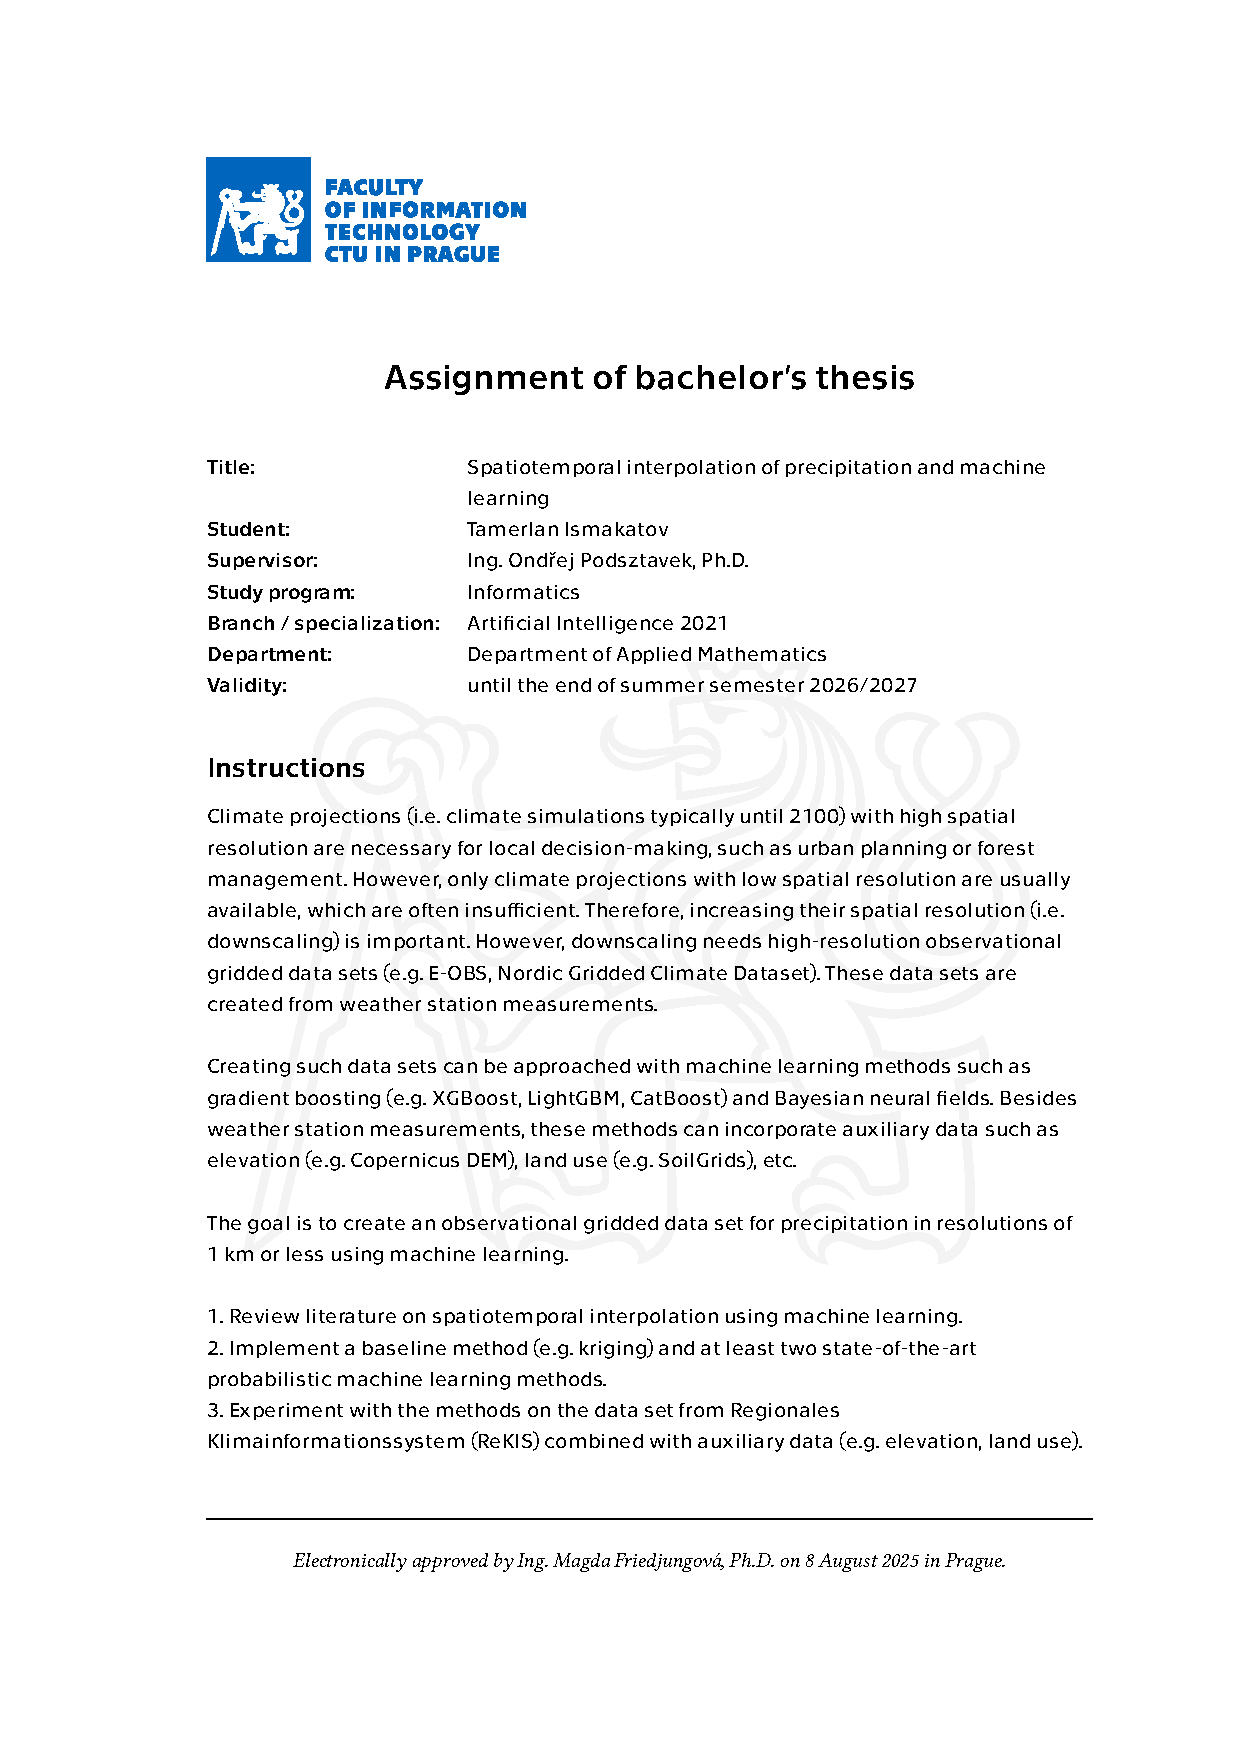
\includepdf[pages={1-}]{ismaktam-assignment.pdf} % replace this file with your thesis assignment generated from ProjectsFIT

\imprintpage % do not remove this command
\stopTOCentries

%%%%%%%%%%%%%%%%%%%
% ACKNOWLEDGMENT
% FILL IN / MODIFY
% This is a place to thank people for helping you. It is common to thank your supervisor.
%%%%%%%%%%%%%%%%%%%
\begin{acknowledgmentpage}
      I would like to express my sincere gratitude to my supervisor,
      Ing.\,Ondřej Podsztavek, Ph.D., for his guidance, patience, and
      constructive feedback throughout the preparation of this thesis.
      I am also deeply grateful to my family for their continuous
      support and encouragement during my studies, and to my friends,
      whose company made this journey enjoyable.
  \end{acknowledgmentpage}
%%%%%%%%%%%%%%%%%%%
% ACKNOWLEDGMENT END
%%%%%%%%%%%%%%%%%%%


%%%%%%%%%%%%%%%%%%%
% DECLARATION
% FILL IN / MODIFY
%%%%%%%%%%%%%%%%%%%
% INSTRUCTIONS
% ENG: choose one of approved texts of the declaration. DO NOT CREATE YOUR OWN. Find the approved texts at https://courses.fit.cvut.cz/SFE/download/index.html#_documents (document Declaration for FT in English)
% CZE/SLO: Vyberte jedno z fakultou schvalenych prohlaseni. NEVKLADEJTE VLASTNI TEXT. Schvalena prohlaseni najdete zde: https://courses.fit.cvut.cz/SZZ/dokumenty/index.html#_dokumenty (prohlášení do ZP)
\begin{declarationpage}
    I hereby declare that the presented thesis is my own work and that I have cited all sources of
information in accordance with the Guideline for adhering to ethical principles when elaborating an
academic final thesis.
I acknowledge that my thesis is subject to the rights and obligations stipulated by the Act No.
121/2000 Coll., the Copyright Act, as amended. In accordance with Section 2373(2) of Act No.
89/2012 Coll., the Civil Code, as amended, I hereby grant a non-exclusive authorization (licence) to
utilize this thesis, including all computer programs that are part of it or attached to it and all
documentation thereof (hereinafter collectively referred to as the "Work"), to any and all persons
who wish to use the Work. Such persons are entitled to use the Work in any manner that does not
diminish the value of the Work and for any purpose (including use for profit). This authorisation is
unlimited in time, territory and quantity.

    I declare that I have used AI tools during the preparation and writing of my thesis. I have verified
the generated content. I confirm that I am aware that I am fully responsible for the content of the
thesis.
\end{declarationpage}
%%%%%%%%%%%%%%%%%%%
% DECLARATION END
%%%%%%%%%%%%%%%%%%%

% Use one of the two following commands. The first prints abstracts+keywords on two pages, the second puts them on one page (if possible). \printonepageabstract can also accept optional argument that specifies a vertical space before both abstracts (the default is 18 mm).
%\printtwopageabstract
\printonepageabstract

%%%%%%%%%%%%%%%%%%%
% SUMMARY
% FILL IN / MODIFY
% OR REMOVE ENTIRELY (upon agreement with your supervisor)
% (appropriate to remove in most theses)
%%%%%%%%%%%%%%%%%%%
% \begin{summarypage}
% \section*{Summary section}
%
% \lipsum[1][1-8]
%
% \section*{Summary section}
%
% \lipsum[2][1-6]
%
% \section*{Summary section}
%
% \lipsum[3]
%
% \section*{Summary section}
%
% \lipsum[2]
%
% \section*{Summary section}
%
% \lipsum[1][1-8] Lorem lorem lorem.
% \end{summarypage}
%%%%%%%%%%%%%%%%%%%
% SUMMARY END
%%%%%%%%%%%%%%%%%%%

\tableofcontents % do not remove this command
%%%%%%%%%%%%%%%%%%%%%%
% list of other contents: figures, tables, code listings, algorithms, etc.
% add/remove commands accordingly
%%%%%%%%%%%%%%%%%%%%%%
\listoffigures % list of figures
\begingroup
\let\clearpage\relax
\listoftables % list of tables. Remove if you do not have any.
\thectufitlistingscommand{} % list of code listings. Remove if you do not have any.
\thectufitlistofalgorithmscommand{} % list of algorithm pseudocodes defined using the algorithm package.
\endgroup
%%%%%%%%%%%%%%%%%%%%%%
% list of other contents END
%%%%%%%%%%%%%%%%%%%%%%

%%%%%%%%%%%%%%%%%%%
% ABBREVIATIONS
% FILL IN / MODIFY
% OR REMOVE ENTIRELY
% List the abbreviations in lexicography order.
%%%%%%%%%%%%%%%%%%%
\chapter{\thectufitabbreviationlabel}

\begin{tabular}{rl}
	DFA   & Deterministic Finite Automaton                 \\
	FA    & Finite Automaton                               \\
	LPS   & Labelled Prüfer Sequence                       \\
	NFA   & Nondeterministic Finite Automaton              \\
	NPS   & Numbered Prüfer Sequence                       \\
	XML   & Extensible Markup Language                     \\
	XPath & XML Path Language                              \\
	XSLT  & eXtensible Stylesheet Language Transformations \\
	W3C   & World Wide Web Consortium
\end{tabular}
%%%%%%%%%%%%%%%%%%%
% ABBREVIATIONS END
%%%%%%%%%%%%%%%%%%%
\resumeTOCentries
\mainmatter\mainmatterinit % do not remove these two commands
%%%%%%%%%%%%%%%%%%%
% THE THESIS
% MODIFY ANYTHING BELOW THIS LINE
%%%%%%%%%%%%%%%%%%%

\chapter{Introduction}
\label{ch:introduction}

High-resolution gridded precipitation data at 1~km resolution and below are
a critical input for hydrological modelling, flood and drought prediction,
climate impact assessment, and agricultural planning.
Producing these grids from observations is difficult: meteorological station
networks are sparse and spatially uneven, leaving large portions of any study
domain without direct measurements.
Converting discrete point observations into the continuous spatial fields
that downstream models require is the central problem of spatial precipitation
interpolation.

Precipitation's statistical properties make standard interpolation methods
inappropriate.
Unlike temperature or pressure, which are continuous and approximately
Gaussian, daily precipitation has a \textbf{mixed discrete-continuous} distribution.
A large fraction of all station-days record exactly zero (dry days), producing
a point mass at zero that cannot be represented by a single linear interpolator over a continuous field.
In the Central European study domain used in this thesis, dry days predominate
across the study period (overall dry-day fraction 51.9\%), though the proportion
varies by season and location, making the zero-inflation problem unavoidable.
Among wet days, precipitation amounts follow a heavy-tailed, right-skewed
distribution, with rare but intense events contributing disproportionately to
the total.

Both properties rule out naive application of standard kriging — a geostatistical method that estimates values at unobserved locations as a weighted average of neighbouring stations, assuming a stationary random field.

The core scientific problem addressed by this thesis is the transformation of
discrete, point-level daily precipitation measurements into continuous,
statistically coherent spatial fields at 1~km resolution over northern and
central Germany
(longitude $9.4^\circ$--$15.9^\circ$\,E, latitude $50.0^\circ$--$53.8^\circ$\,N,
EPSG:3035).
The study domain is served by the ReKIS regional climate network, comprising
2{,}458 stations with daily records spanning 1961--2023.

Three properties of the daily precipitation distribution require explicit treatment.
First, the \textbf{zero} inflation must be handled through either a two-stage model
that separates occurrence from amounts, or a unified framework that accommodates
the mixed distribution directly.
Second, the \textbf{non-stationarity of the mean}, caused by both the seasonal
cycle and orographic forcing, violates the stationarity assumption of standard
kriging (see Chapter~\ref{ch:theory}) and must be removed before spatial correlation can be modelled.
Third, the \textbf{right-skewness} of wet-day amounts requires a
variance-stabilising transformation if the kriging uncertainty estimates are
to be physically meaningful.

This thesis has three objectives:

\begin{enumerate}
    \item \textbf{Implement and validate Ordinary Kriging as a baseline.}
    A complete preprocessing and interpolation pipeline is developed to handle
    the statistical properties of daily precipitation that standard kriging
    cannot address directly.
    The pipeline is evaluated by cross-validation using a proper scoring
    rule that assesses both point accuracy and uncertainty calibration.

    \item \textbf{Assess the role of terrain elevation as an auxiliary predictor.}
    Elevation data from the Copernicus Digital Elevation Model are incorporated
    into the interpolation of climatological monthly normals.
    Cross-validation quantifies whether the orographic precipitation gradient
    in the study domain can be captured and whether doing so reduces
    interpolation error.

    \item \textbf{Contextualise results relative to machine learning alternatives.}
    Gradient boosting and Bayesian neural field approaches are implemented
    and compared as non-geostatistical alternatives.
    The geostatistical approach is the interpretable, physically motivated
    baseline; gradient boosting and the neural field model test whether
    data-driven flexibility improves on it.
\end{enumerate}

\textbf{Chapter~2} reviews the theoretical background of the three methods examined in this thesis.

\textbf{Chapter~3} describes the study domain and its data sources.

\textbf{Chapter~4} presents the implementation of the Ordinary Kriging pipeline.

\textbf{Chapter~5} presents the gradient boosting implementation for
spatial precipitation interpolation, including feature construction and
hyperparameter selection.

\textbf{Chapter~6} presents the Bayesian Neural Field implementation
applied to the same interpolation task.

\textbf{Chapter~7} compares the three methods on common evaluation metrics,
examines the gridded outputs, and discusses the trade-offs between
geostatistical interpretability and data-driven flexibility.

\textbf{Chapter~8} summarises the main findings and outlines directions for
future work.

\bigskip
\noindent\textbf{Code and data availability.}
The complete codebase developed for this thesis — preprocessing
pipelines, the three interpolation models, evaluation notebooks and
the scripts that build the gridded product — is publicly available in
the project's GitHub repository~\cite{thesisRepo}.

\chapter{Theoretical Background}
\label{ch:theory}

%=============================================================================
\section{Geostatistical framework: Ordinary Kriging}
\label{sec:theory-kriging}
%=============================================================================

\subsection{Spatial Random Fields}
\label{sec:random_fields}

Geostatistics treats a spatially distributed variable (such as daily
precipitation) as a realisation of a \textbf{spatial random field} (also
called a random function or stochastic process) $\{Z(\mathbf{s}) :
\mathbf{s} \in \mathcal{D}\}$, where $\mathbf{s} \in \mathbb{R}^2$ denotes a
spatial location and $\mathcal{D}$ is the study domain
\cite{matheron1963principles, cressie1993}.
Under this view, the observed precipitation values at weather stations are
treated as a single realisation of this random field, rather than as
deterministic quantities.

Hofstra et al.~\cite{hofstra2008comparison} describe kriging as a stochastic method in
which the interpolated value is a linear combination of nearby station
measurements, with weights chosen to minimise the mean squared prediction error
conditional on a model of spatial variability (the variogram).
Because these weights depend entirely on the distance-based covariance
structure, kriging implicitly relies on \textbf{spatial autocorrelation}: the
tendency of observations at nearby locations to be more similar than those at
distant locations.
Without such structure, the variogram would carry no information and there
would be no basis for predicting values at unobserved locations from nearby
measurements.
The following sections formalise this dependence structure through stationarity
assumptions and the variogram.


\subsection{Stationarity}
\label{sec:stationarity}

To make inference about a random field from a single realisation (the only
data available in practice), some regularity in the spatial structure
must be assumed.
The standard assumption is \textbf{stationarity}: the statistical properties
of the field do not depend on absolute location but only on the spatial
separation between points \cite{hofstra2008comparison, haylock2008european}.

\subsubsection{Second-Order Stationarity}

A random field is said to be \textit{second-order stationary} (or
\textit{weakly stationary}) if:

\begin{enumerate}
    \item The mean is constant: $E[Z(\mathbf{s})] = \mu$ for all
    $\mathbf{s} \in \mathcal{D}$.
    \item The covariance depends only on the separation vector $\mathbf{h}$:
    $\text{Cov}(Z(\mathbf{s}), Z(\mathbf{s} + \mathbf{h})) = C(\mathbf{h})$
    for all $\mathbf{s}$.
\end{enumerate}

\noindent Under this assumption, the covariance function $C(\mathbf{h})$
captures the full spatial dependence structure, and it can be estimated from
the data by treating all pairs of stations separated by lag $\mathbf{h}$ as
equivalent replicates \cite{cressie1993}.

\subsubsection{Intrinsic Stationarity}

Second-order stationarity requires a finite variance, which may not hold for
all natural processes.
A weaker condition, \textbf{intrinsic stationarity}, assumes only that the
variance of the increment $Z(\mathbf{s}+\mathbf{h}) - Z(\mathbf{s})$
depends on the lag~$\mathbf{h}$ alone and not on the location~$\mathbf{s}$:

\begin{equation}
    \text{Var}\bigl[Z(\mathbf{s} + \mathbf{h}) - Z(\mathbf{s})\bigr]
    = 2\gamma(\mathbf{h})
    \label{eq:intrinsic_stationarity}
\end{equation}

\noindent where $\gamma(\mathbf{h})$ is the \textbf{semi-variogram} (or simply
the variogram).
Intrinsic stationarity is sufficient for ordinary kriging and is the assumption
adopted throughout this work.
As Deutsch and Journel~\cite{deutsch1998gslib} note (Section~II.1.3, eq.~II.11), the
variogram definition requires only second-order stationarity of the random
function increments, a condition they call the \textit{``intrinsic hypothesis''}, which
is a weaker requirement than full second-order stationarity of the field
itself \cite{matheron1963principles, cressie1993}.

In the context of daily precipitation, raw observations violate stationarity in
two principal ways \cite{haylock2008european, hofstra2008comparison}.
The seasonal cycle introduces a large-scale trend, with the mean and
variance differing substantially between summer and winter months.
Orographic forcing also creates a spatial gradient in precipitation
climatology, with elevated regions receiving systematically more rainfall
than lowland areas \cite{haylock2008european}.
Both sources of non-stationarity must be removed before kriging can be
applied.


\subsection{The Variogram}
\label{sec:variogram}

\subsubsection{Definition and Estimation}

The semi-variogram $\gamma(\mathbf{h})$ defined in
Equation~\eqref{eq:intrinsic_stationarity} measures how the variance between
two observations grows with increasing separation $\mathbf{h}$.
In practice, the lag is treated as a scalar distance $h = \|\mathbf{h}\|$
under the isotropy assumption discussed in Section~\ref{sec:isotropy}.

The \textbf{empirical} (or \textit{experimental}) semi-variogram is estimated
from the data using the method-of-moments estimator
\cite{matheron1963principles}:

\begin{equation}
    \hat{\gamma}(h) =
    \frac{1}{2\,N(h)}
    \sum_{(i,j)\,:\,\|\mathbf{s}_i - \mathbf{s}_j\| \approx h}
    \bigl[Z(\mathbf{s}_i) - Z(\mathbf{s}_j)\bigr]^2
    \label{eq:empirical_variogram}
\end{equation}

\noindent where $N(h)$ is the number of station pairs whose distance falls
within the lag bin centred on $h$ \cite{cressie1993, haylock2008european}.
At least 30 pairs per lag bin are recommended to achieve statistical stability
\cite{cressie1993}.

\subsubsection{Key Parameters: Nugget, Sill, and Range}

A fitted variogram model is characterised by three parameters with clear
physical interpretations (Figure~\ref{fig:variogram_diagram}):

\begin{description}
    \item[Nugget ($c_0$)]
    The discontinuity at the origin: the variance between two measurements at
    the same location is theoretically zero, but empirical variograms typically
    show a positive intercept due to (i) measurement error in rain gauges and
    (ii) sub-grid spatial variability at scales smaller than the station
    spacing \cite{webster2007geostatistics}.
    For daily precipitation, the nugget reflects the fundamental
    unpredictability of highly localised convective cells.

    \item[Sill ($c_0 + c_1$)]
    The plateau reached by the variogram at large separations, equal to the
    overall variance of the transformed variable \cite{cressie1993}.
    The partial sill $c_1 = (c_0 + c_1) - c_0$ is the spatially structured
    component of the variance.
    For precipitation, the sill is larger for convective summer storms (high
    local variability) than for widespread stratiform winter events
    \cite{hofstra2008comparison}.

    \item[Range ($a$)]
    The separation distance at which the variogram reaches (or effectively
    reaches) the sill; beyond this distance, observations are spatially
    uncorrelated \cite{webster2007geostatistics}.
    Physically, the range reflects the spatial extent of the dominant weather
    system.
\end{description}

\noindent The \textbf{nugget-to-sill ratio} $c_0 / (c_0 + c_1)$ is a useful
diagnostic: values below 0.25 indicate strong spatial structure where kriging
adds substantial information beyond the sample mean, while values above 0.5
indicate that most variance is unstructured noise
\cite{webster2007geostatistics}.

\begin{figure}[ht]
    \centering
    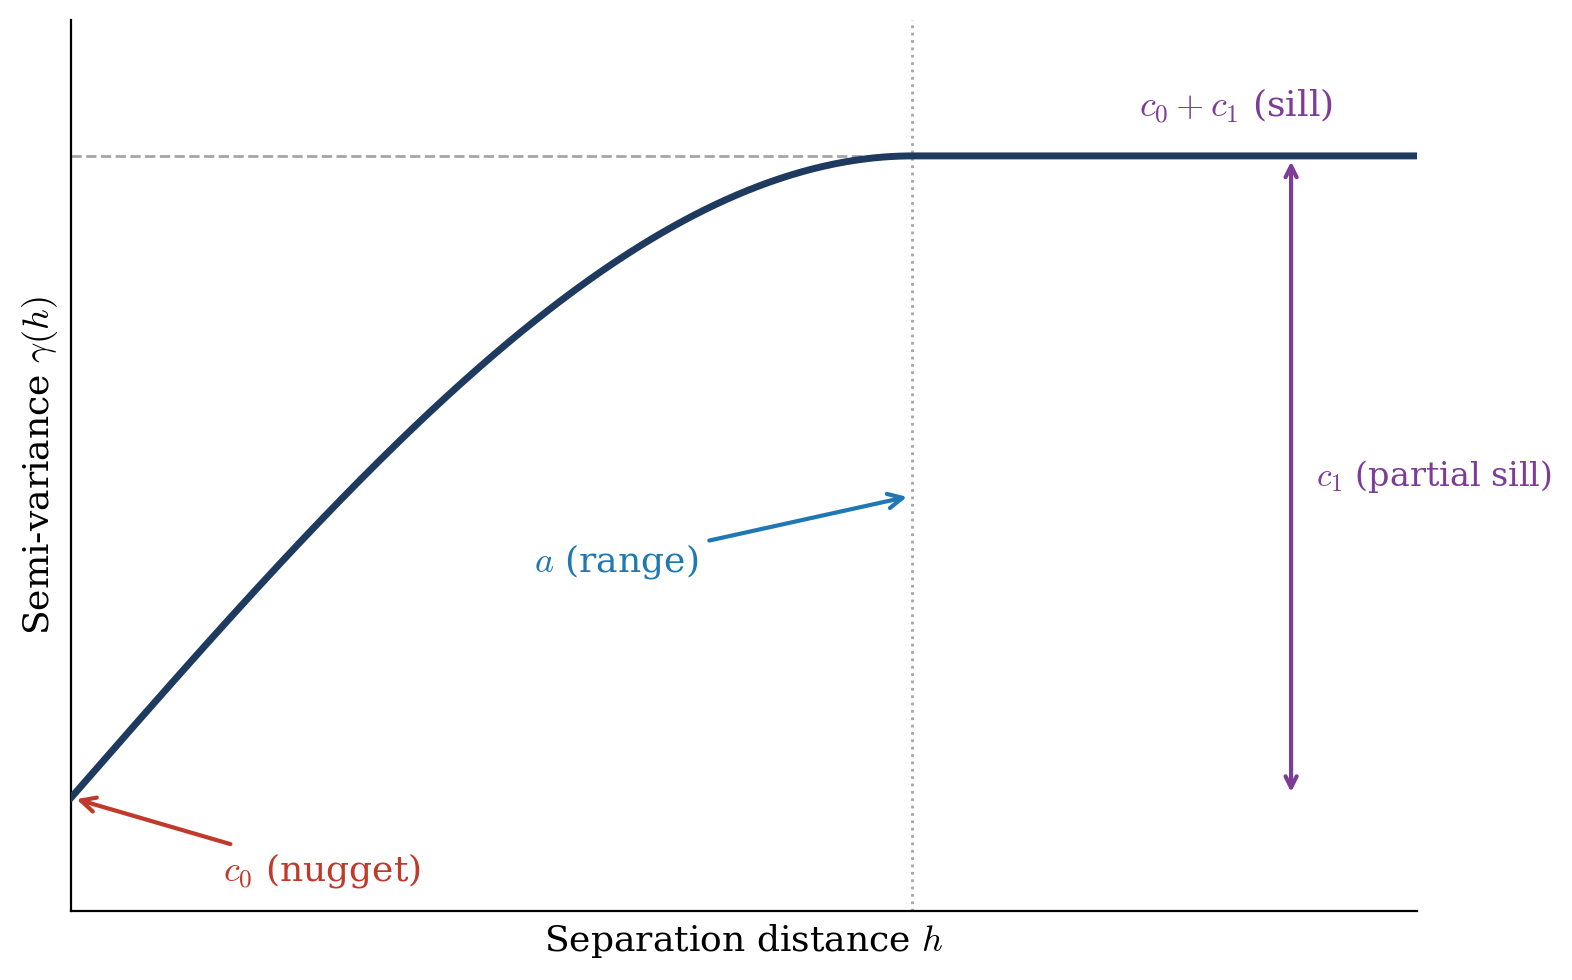
\includegraphics[width=0.85\textwidth]{images/02/variogram_diagram}
    \caption[Conceptual structure of a spherical variogram]{Conceptual structure of a spherical variogram, illustrating
    the three characteristic parameters: nugget $c_0$, partial sill $c_1$,
    sill $c_0 + c_1$, and range $a$; redrawn after Cressie~\cite{cressie1993}
    and Webster and Oliver~\cite{webster2007geostatistics}}
    \label{fig:variogram_diagram}
\end{figure}

\subsection{Variogram Models}
\label{sec:variogram_models}

A theoretical parametric model must be fitted to the empirical variogram before
it can be used in kriging, because the weights are computed from variogram
values at arbitrary distances not necessarily covered by the data.
The model must also be a \textit{valid} (conditionally negative
semi-definite) variogram, which guarantees that the kriging covariance
matrix is positive definite and the estimation variance is non-negative
\cite{cressie1993}.
All three models listed below satisfy this condition.

Three models are commonly used for precipitation
\cite[see][ch.~2--4]{cressie1993, webster2007geostatistics}:

\paragraph{Spherical model}

\begin{equation}
    \gamma_{\text{sph}}(h) =
    \begin{cases}
        c_0 + c_1 \!\left[\dfrac{3h}{2a} - \dfrac{1}{2}\!\left(\dfrac{h}{a}\right)^{\!3}\right]
        & h \le a \\[8pt]
        c_0 + c_1 & h > a
    \end{cases}
    \label{eq:spherical}
\end{equation}

The spherical model reaches the sill at a finite distance $a$ and is linear
near the origin, making it appropriate for variables that exhibit a sharp
decorrelation beyond a characteristic scale.
Haylock et al.~\cite{haylock2008european} recommend the spherical model for precipitation
\textit{occurrence} (indicator kriging).

\paragraph{Exponential model}

\begin{equation}
    \gamma_{\text{exp}}(h) = c_0 + c_1 \left[1 - \exp\!\left(-\frac{h}{a}\right)\right]
    \label{eq:exponential}
\end{equation}

The exponential model approaches the sill asymptotically; the effective range
(at which $\gamma$ reaches 95\% of the sill) is $3a$.
Unlike the spherical model, which reaches the sill at a finite distance,
the exponential model never fully decorrelates, making it appropriate for
precipitation \textit{amounts}, where spatial correlation
decays gradually over long distances \cite{haylock2008european}.

\paragraph{Gaussian model}

\begin{equation}
    \gamma_{\text{gau}}(h) = c_0 + c_1 \left[1 - \exp\!\left(-\frac{h^2}{a^2}\right)\right]
    \label{eq:gaussian}
\end{equation}

The Gaussian model is infinitely differentiable at the origin, implying
an extremely smooth spatial field.
While suitable for temperature fields, it is generally less appropriate for
precipitation because the parabolic behaviour near $h = 0$ tends to
underestimate short-range variability \cite{cressie1993}.

\subsubsection{Model Selection and Global Fitting}

In the E-OBS methodology, model parameters are estimated by the
\textbf{Marquardt method}~\cite{haylock2008european}, a weighted least squares
fit minimising the discrepancy between empirical and theoretical
variograms, with weights proportional to the number of station pairs per
lag bin:
\begin{equation}
  (c_0^*,\, c_1^*,\, a^*)
  = \argmin_{c_0,\, c_1,\, a}
    \sum_{k=1}^{K}
    N_k \!\left[\hat{\gamma}(h_k) - \gamma_{\theta}(h_k)\right]^{2},
  \label{eq:marquardt-variogram}
\end{equation}
where $N_k$ is the number of station pairs in bin~$k$, $\hat{\gamma}(h_k)$ is the
empirical semi-variance, and $\gamma_{\theta}(h_k)$ is the theoretical model.
Weighting by $N_k$ gives larger influence to well-populated bins, following the
E-OBS fitting procedure, which \textit{``gave more weight to those points in the
experimental variogram that were calculated from more station pairs''}
\cite[p.~5]{haylock2008european}.
Hofstra et al.~\cite{hofstra2008comparison} tested all three models and selected the best
fit using the chi-squared statistic.

A key practical finding is that a \textbf{global variogram}, fitted once by
pooling semi-variance estimates from many days, outperforms day-specific
variograms in cross-validation.
A variogram estimated from a single day's data (typically 100--200 pairs) is too
noisy: the standard error of the estimator is inversely proportional to
$\sqrt{N_k}$, where $N_k$ is the number of pairs at lag $k$.
Pooling across days provides a robust climatological
estimate of the spatial correlation structure
\cite{hofstra2008comparison, haylock2008european}.
Cross-validation experiments in both Haylock et al.~\cite{haylock2008european}
and Hofstra et al.~\cite{hofstra2008comparison} confirmed that a single global
variogram outperforms per-month fits: monthly subsets contain too few pairs for
a reliable estimate, and once precipitation is normalised by the monthly
climatology the residual correlation shape changes little between
seasons \cite{haylock2008european}.
This approach is adopted in the implementation described in
Chapter~\ref{ch:kriging}.


\subsection{Isotropy}
\label{sec:isotropy}

A variogram is called \textbf{isotropic} if it depends only on the distance
$h = \|\mathbf{h}\|$ and not on the direction of $\mathbf{h}$.
Anisotropy occurs when spatial correlation is stronger in one direction than
another (for example, along prevailing wind patterns or mountain ridges).

Hofstra et al.~\cite{hofstra2008comparison} tested for anisotropy in European daily
precipitation but found that computing directional variograms introduced more
uncertainty than it resolved, because fewer station pairs fall within each
directional bin.
They concluded that an omnidirectional (isotropic) variogram is more
appropriate for operational daily precipitation interpolation, and this choice
is followed throughout the present work.


\subsection{Ordinary Kriging as a Best Linear Unbiased Estimator}
\label{sec:kriging_blue}

\subsubsection{The Kriging Estimator}

Given observations $\{Z(\mathbf{s}_1), \ldots, Z(\mathbf{s}_n)\}$ at $n$
stations, the ordinary kriging estimator at an unobserved location $\mathbf{s}_0$
is defined as a \textbf{linear} combination of the observed values:

\begin{equation}
    \hat{Z}(\mathbf{s}_0) = \sum_{i=1}^{n} w_i \, Z(\mathbf{s}_i)
    \label{eq:kriging_estimator}
\end{equation}

\noindent where $w_i$ are weights to be determined
\cite{matheron1963principles, hofstra2008comparison}.

\subsubsection{Unbiasedness and the Weight Constraint}

For the estimator to be \textbf{unbiased}
($E[\hat{Z}(\mathbf{s}_0)] = E[Z(\mathbf{s}_0)] = \mu$), the weights must
sum to unity:

\begin{equation}
    \sum_{i=1}^{n} w_i = 1
    \label{eq:weight_constraint}
\end{equation}

\noindent This constraint ensures that kriging does not systematically
over- or under-predict the (unknown) spatial mean
\cite{cressie1993, hofstra2008comparison}.

\subsubsection{Optimality: Minimising the Estimation Variance}

The weights are chosen to minimise the \textbf{estimation variance}
(mean squared error):

\begin{equation}
    \sigma^2_{\text{OK}}(\mathbf{s}_0)
    = \text{Var}\!\left[\hat{Z}(\mathbf{s}_0) - Z(\mathbf{s}_0)\right]
    \label{eq:kriging_variance_def}
\end{equation}

\noindent subject to Constraint~\eqref{eq:weight_constraint}.
This is a constrained optimisation problem solved via a Lagrange multiplier
$\lambda$ \cite{cressie1993, webster2007geostatistics}.

\subsubsection{The Kriging System}

Taking partial derivatives with respect to each $w_i$ and setting them to
zero yields the \textbf{ordinary kriging system} in matrix form
\cite{cressie1993, webster2007geostatistics, deutsch1998gslib}:

\begin{equation}
    \begin{bmatrix}
        \mathbf{K} & \mathbf{1} \\
        \mathbf{1}^\top & 0
    \end{bmatrix}
    \begin{bmatrix}
        \mathbf{w} \\ \lambda
    \end{bmatrix}
    =
    \begin{bmatrix}
        \mathbf{k} \\ 1
    \end{bmatrix}
    \label{eq:kriging_system}
\end{equation}

\noindent where:
\begin{itemize}
    \item $K_{ij} = \gamma(\|\mathbf{s}_i - \mathbf{s}_j\|)$ is the
    $(n \times n)$ variogram matrix between all pairs of station locations,
    \item $k_i = \gamma(\|\mathbf{s}_i - \mathbf{s}_0\|)$ is the
    $(n \times 1)$ vector of variogram values between each station and
    the prediction point,
    \item $\mathbf{1}$ is an $n$-vector of ones enforcing
    Constraint~\eqref{eq:weight_constraint},
    \item $\lambda$ is the Lagrange multiplier.
\end{itemize}

Solving this $(n+1) \times (n+1)$ linear system yields the optimal weights
$\mathbf{w}^*$ and the Lagrange multiplier $\lambda^*$.
The associated kriging variance is:

\begin{equation}
    \sigma^2_{\text{OK}}(\mathbf{s}_0)
    = \sum_{i=1}^{n} w_i^* \, \gamma(\|\mathbf{s}_i - \mathbf{s}_0\|)
    + \lambda^*
    \label{eq:kriging_variance}
\end{equation}

\noindent This expression shows that the estimation uncertainty is large when
the prediction point is far from all stations (large $\gamma$ values) and
small when stations are nearby \cite{cressie1993}.

In summary, ordinary kriging is the BLUE because it is
\cite{matheron1963principles, cressie1993, webster2007geostatistics}:
\begin{itemize}
    \item \textbf{Linear} — the estimator is a weighted sum of observations
    (Equation~\eqref{eq:kriging_estimator}),
    \item \textbf{Unbiased} — the weight constraint ensures zero expected error
    (Equation~\eqref{eq:weight_constraint}),
    \item \textbf{Best} — the weights minimise the estimation variance among
    all linear unbiased estimators
    \cite{matheron1963principles, cressie1993}.
\end{itemize}

\noindent The BLUE property holds under the intrinsic stationarity assumption
and does not require a Gaussian distribution for the data.
Under approximate Gaussianity, the kriging variance
$\sigma^2_{\text{OK}}$ additionally acquires a probabilistic interpretation
as a prediction interval.

\subsection{Two-stage decomposition for zero-inflated data}
\label{sec:kriging-indicator}

The first and most fundamental decision when applying kriging to precipitation
is to decompose the task into two independent questions
rather than apply a single kriging model to the mixed distribution
\cite{journel1983indicator, haylock2008european}:

\begin{equation}
  Z(\mathbf{s}_0) =
    \underbrace{I(\mathbf{s}_0)}_{\text{stage 1: rain or not?}}
    \times
    \underbrace{A(\mathbf{s}_0)}_{\text{stage 2: how much?}}
  \label{eq:two-stage}
\end{equation}

In \textbf{Stage~1}, each observation is converted to a binary variable:
$I(\mathbf{s}_i, t) = 1$ if precipitation exceeds a wet-day threshold $\tau$, and $I = 0$ otherwise.
Ordinary Kriging is applied to these indicators and produces at each grid point a
value $\hat{p}(\mathbf{s}_0)$ interpreted as the probability of observing a wet day
\cite{hofstra2008comparison}.
Because ordinary kriging does not constrain predictions to $[0,1]$, values
slightly outside this range can occur near the boundaries of the wet--dry transition;
in practice a decision threshold $p^{\star}$ classifies a cell as rainy if
$\hat{p}(\mathbf{s}_0) > p^{\star}$.

The indicator semi-variogram $\gamma_I(h)$ describes how quickly agreement
in wet-day occurrence decays with spatial lag.
Following the global-variogram principle, a single spherical model is fitted by
pooling empirical indicator semi-variance across all days in the study period,
excluding constant days (all-wet or all-dry) on which the indicator has zero
variance.
Haylock et al.~\cite{haylock2008european} found that a global variogram produces
better interpolation skill than day-specific fits because the larger sample
provides a more statistically robust estimate of the spatial correlation
structure.
The fitted parameters of the global indicator variogram are applied
identically to every day, ensuring stable predictions even on days with
few wet stations where a per-day fit would be unreliable.

Ordinary Kriging (Section~\ref{sec:kriging_blue}) is applied to the binary
indicators, yielding the weighted estimate
$\hat{p}(\mathbf{s}_0, t) = \sum_{i=1}^{n} w_i\, I(\mathbf{s}_i, t)$
with weights from the kriging system~\eqref{eq:kriging_system}.
Because the input values are binary, this estimate is interpreted as the
wet-day probability at the target cell. The final first-stage decision is therefore
\begin{equation}
  \widehat{I}(\mathbf{s}_0, t)
  =
  \mathbf{1}\!\left[\hat{p}(\mathbf{s}_0, t) > p^{\star}\right].
  \label{eq:indicator-decision}
\end{equation}
Stage~1 thus outputs a binary wet/dry mask rather than precipitation amount in
millimetres.

In \textbf{Stage~2}, kriging is applied only to the positive observations (at those
stations where rain was recorded) and only for those grid cells where Stage~1 predicted
rainfall. The zero-inflation problem is resolved: the remaining mathematics operates
exclusively on the continuous distribution of positive precipitation amounts.

This coupling between the two stages can be written explicitly as
\begin{equation}
  \hat{Z}(\mathbf{s}_0, t)
  =
  \widehat{I}(\mathbf{s}_0, t)\, \hat{A}(\mathbf{s}_0, t),
  \label{eq:two-stage-predictor}
\end{equation}
where $\hat{A}(\mathbf{s}_0, t)$ is the second-stage amount prediction obtained only from
wet stations. If Stage~1 classifies the cell as dry, the final prediction is set to zero.

A practical limitation of the two-stage approach is that the final uncertainty
estimate is typically based only on Stage~2 (amount kriging) and does not account for the
classification uncertainty from Stage~1. Both questions, ``is it raining?'' and ``how
much?'', carry their own uncertainty, and combining them remains a non-trivial problem
\cite{haylock2008european}.

\subsection{Climatological normalisation}
\label{sec:theory-quota}

Having split the task into two stages, non-stationarity of the mean remains.
Consider the following: 10~mm of rainfall in June in a mountain foothills region is an
unremarkable event, roughly one sixth of the typical monthly normal. The same 10~mm in
December in Prague is anomalously high, twice the average. Kriging has no knowledge of
this distinction: both observations enter the interpolation equation with the same value
of ``10''.

The solution proposed in the E-OBS methodology \cite{haylock2008european} is to
replace absolute precipitation values with a \textbf{dimensionless climatological ratio}
indicating what fraction of the climatological monthly normal fell on that day:

\begin{equation}
  Q(\mathbf{s}_i, t) = \frac{Z(\mathbf{s}_i, t)}{\bar{M}(\mathbf{s}_i,\; m(t))}
  \label{eq:quota}
\end{equation}

where $\bar{M}(\mathbf{s}_i, m)$ is the long-term climatological monthly precipitation
total at station $\mathbf{s}_i$ in month $m$. This quantity is called the
\emph{quota} in the original E-OBS paper \cite{haylock2008european};
this thesis adopts the term \emph{ratio}, which is more transparent to a
general reader, but the symbol $Q$ and the construction are preserved.
After this normalisation, the expected value of the ratio is approximately constant
across all stations in any month: non-stationarity of the mean is eliminated,
and the kriging stationarity assumption is satisfied.
This procedure is an instance of \textbf{Climatologically Aided Interpolation}
(CAI) \cite{willmott1995cai}; the multiplicative ratio replaces the additive
deviation used for temperature, since precipitation variance scales with
the mean.

\subsection{Precipitation transforms}
\label{sec:kriging-nst}

After detrending, the wet-day ratios $Q$ are positive and approximately stationary,
but their distribution remains right-skewed and heavy-tailed
\cite{hofstra2008comparison, cecinati2017}.
Under Gaussianity, Ordinary Kriging additionally becomes the Best Linear Unbiased
\emph{Predictor} (BLUP), and the kriging variance acquires a correct probabilistic
interpretation as a prediction interval \cite{cressie1993, deutsch1998gslib}.
This motivates testing transforms that push the ratios closer to normality
\cite{cecinati2017}.
Three candidates are considered, each mapping the ratio to a working
variable~$z$ in a different \emph{z-space}:

\begin{enumerate}
  \item \textbf{None (raw ratio).}  The simplest option: $z = Q$.  The
        variogram is fitted directly on ratio values; no back-transformation is
        needed beyond the final multiplication
        $\hat{Z} = \hat{Q}\,\bar{M}$.

  \item \textbf{Log transform.}  $z = \log(Q + \delta)$ with a small
        offset $\delta$ to prevent divergence for near-zero ratios.
        This is a parametric transform that implicitly assumes an
        approximately log-normal distribution.  Back-transformation is
        $\hat{Q} = \exp(\hat{z}) - \delta$.

  \item \textbf{Normal Score Transform (NST).}  A rank-based transform
        mapping $Q$ to $\mathcal{N}(0,1)$ via the empirical CDF
        \cite{cecinati2017, deutsch1998gslib}.
\end{enumerate}

Each transform produces a different z-space with its own scale, so the
variogram parameters (sill, range, nugget) are not comparable across
transforms, and each combination of transform and variogram model must
be evaluated independently.

%=============================================================================
\section{Gradient boosting for spatial regression}
\label{sec:theory-gbm}
%=============================================================================

\subsection{Gradient boosting}
\label{sec:theory-gbm-general}

Gradient boosting is a supervised learning framework that constructs a
predictor as an additive ensemble of weak learners, typically shallow
regression trees \cite{friedman2001greedy}. Starting from a constant initial
prediction, the model is updated stage-wise:
\begin{equation}
  F_t(\mathbf{x}) = F_{t-1}(\mathbf{x}) + \nu \, h_t(\mathbf{x}),
  \label{eq:gbm-additive}
\end{equation}
where each tree $h_t$ is fitted to the negative gradient of a differentiable
loss function evaluated at the current ensemble's predictions, and the
learning rate $\nu \in (0, 1]$ controls the contribution of each new tree.
This is equivalent to gradient descent in the function space of the
ensemble: the negative gradient is the pseudo-residual that points to where
the current model has the largest error.
Unlike kriging, which assumes a stationary spatial random field, gradient
boosting does not require a parametric distributional model and admits
auxiliary covariates (e.g.\ elevation, soil properties) directly as input
features.
The same two-stage decomposition for zero-inflated precipitation
introduced in Section~\ref{sec:kriging-indicator} carries over to gradient
boosting, with a binary classifier and a quantile regression model
replacing indicator and amount kriging respectively.

\subsection{LightGBM}
\label{sec:theory-lgbm}

LightGBM \cite{ke2017lightgbm} is a gradient boosting library designed for
training speed and low memory use. It introduces several optimisations over
the classical algorithm:
\begin{itemize}
  \item \textbf{Leaf-wise tree growth:} instead of growing all leaves at the
    same depth, the leaf with the largest expected loss reduction is split
    first, so the tree deepens where the loss is largest.
  \item \textbf{Histogram-based splitting:} continuous feature values are
    discretised into a fixed number of bins, reducing the cost of finding
    the best split from $\mathcal{O}(n)$ to $\mathcal{O}(\#\text{bins})$.
  \item \textbf{Gradient-Based One-Side Sampling (GOSS):} retains all
    instances with large gradients and randomly subsamples those with small
    gradients. The most informative samples are kept and training cost
    drops with the subsample size.
  \item \textbf{Exclusive Feature Bundling (EFB):} combines mutually exclusive
    sparse features into a single feature, lowering effective dimensionality.
  \item \textbf{Built-in regularisation:} L1/L2 weight penalties, row and
    feature subsampling, leaf-count constraints, and early stopping on a
    validation set jointly control overfitting.
\end{itemize}
These optimisations let LightGBM scale to spatial precipitation problems
in which the number of station-day records reaches tens of millions.

\subsection{Quantile regression for probabilistic prediction}
\label{sec:theory-gbm-quantile}

A standard regression model returns a point estimate $\hat{y}(\mathbf{x})$,
which is insufficient for evaluation under a proper scoring rule such as
CRPS (Section~\ref{sec:theory-metrics}): the latter requires a full
predictive distribution, not a single value.
Quantile regression \cite{koenker1978regression} extends regression by
estimating conditional quantiles directly. For a target quantile level
$\tau \in (0, 1)$, the \textbf{pinball loss} (or check function)
\begin{equation}
  \rho_\tau(y - \hat{y})
    = \begin{cases}
      \tau\,(y - \hat{y})        & \text{if } y \geq \hat{y}, \\
      (\tau - 1)\,(y - \hat{y})  & \text{if } y < \hat{y},
    \end{cases}
  \label{eq:pinball}
\end{equation}
penalises under- and over-predictions asymmetrically in proportion to
$\tau$ and $1 - \tau$.
The conditional $\tau$-quantile estimator is then defined as the predictor
that minimises the average pinball loss over the training set
\cite{koenker1978regression}:
\begin{equation}
  \hat{f}_\tau
    = \argmin_{f \in \mathcal{F}}\,
      \frac{1}{n}\sum_{i=1}^{n} \rho_\tau\!\bigl(y_i - f(\mathbf{x}_i)\bigr).
  \label{eq:quantile-estimator}
\end{equation}
LightGBM supports the pinball loss as a built-in objective, so a separate
model can be trained for each desired quantile level $\tau$.
Predicting on a discrete grid of quantile levels yields an approximation
of the conditional predictive distribution, which serves as the ensemble
required for CRPS evaluation.
A closely related application of this approach is the satellite--gauge
precipitation merging study of Tyralis et al.~\cite{tyralis2023lightgbm},
who showed that LightGBM with quantile regression provides skilful
probabilistic predictions of daily precipitation, particularly at extreme
upper quantiles relevant for flood forecasting.

%=============================================================================
\section{Bayesian Neural Fields}
\label{sec:theory-bayesnf}
%=============================================================================

Ordinary kriging models a single scalar field with a globally stationary
semivariogram fitted to one variable, so auxiliary information such as
elevation, soil type, or seasonal regime can only be injected indirectly
through transforms and detrending stages. Bayesian Neural Fields (BayesNF)
\cite{saad2024bnf} replace this picture with a single Bayesian neural
network that maps spatiotemporal coordinates and arbitrary covariates to
a full predictive distribution, and that learns the covariance structure
of the field from the data rather than committing to a fixed parametric
form in advance.

\subsection{Architecture}
\label{sec:theory-bayesnf-arch}

BayesNF is a coordinate-based neural network: each input is the raw
$(\mathbf{s}, t, \mathbf{x}(\mathbf{s},t))$ tuple of location, time, and
covariates, and the output parameterises a distribution over the
observable field value $Y(\mathbf{s}, t)$. Because the network is
universal, the same backbone serves any spatiotemporal target without
manual redesign of the covariance model. Following Saad et al.\
\cite{saad2024bnf}, the model is hierarchical: a latent field
$F(\mathbf{s},t)$ together with global parameters $\Theta_f, \Theta_y$
defines the prior, and observations follow
\begin{equation}
  Y(\mathbf{s},t) \mid F(\mathbf{s},t), \Theta_y
    \;\sim\; \mathrm{Dist}\!\bigl(g(F(\mathbf{s},t)), \Theta_y\bigr),
  \label{eq:bnf-observation-model}
\end{equation}
where $\mathrm{Dist}$ is a configurable observation family and $g$ links
the latent field to its parameter~\cite{saad2024bnf}.
Figure~\ref{fig:bayesnf-architecture} shows the overall layer stack and
the parameters of the latent field $\theta_f$ and observation
model~$\theta_y$; the remainder of this section describes each layer in
turn.

\begin{figure}[ht]
    \centering
    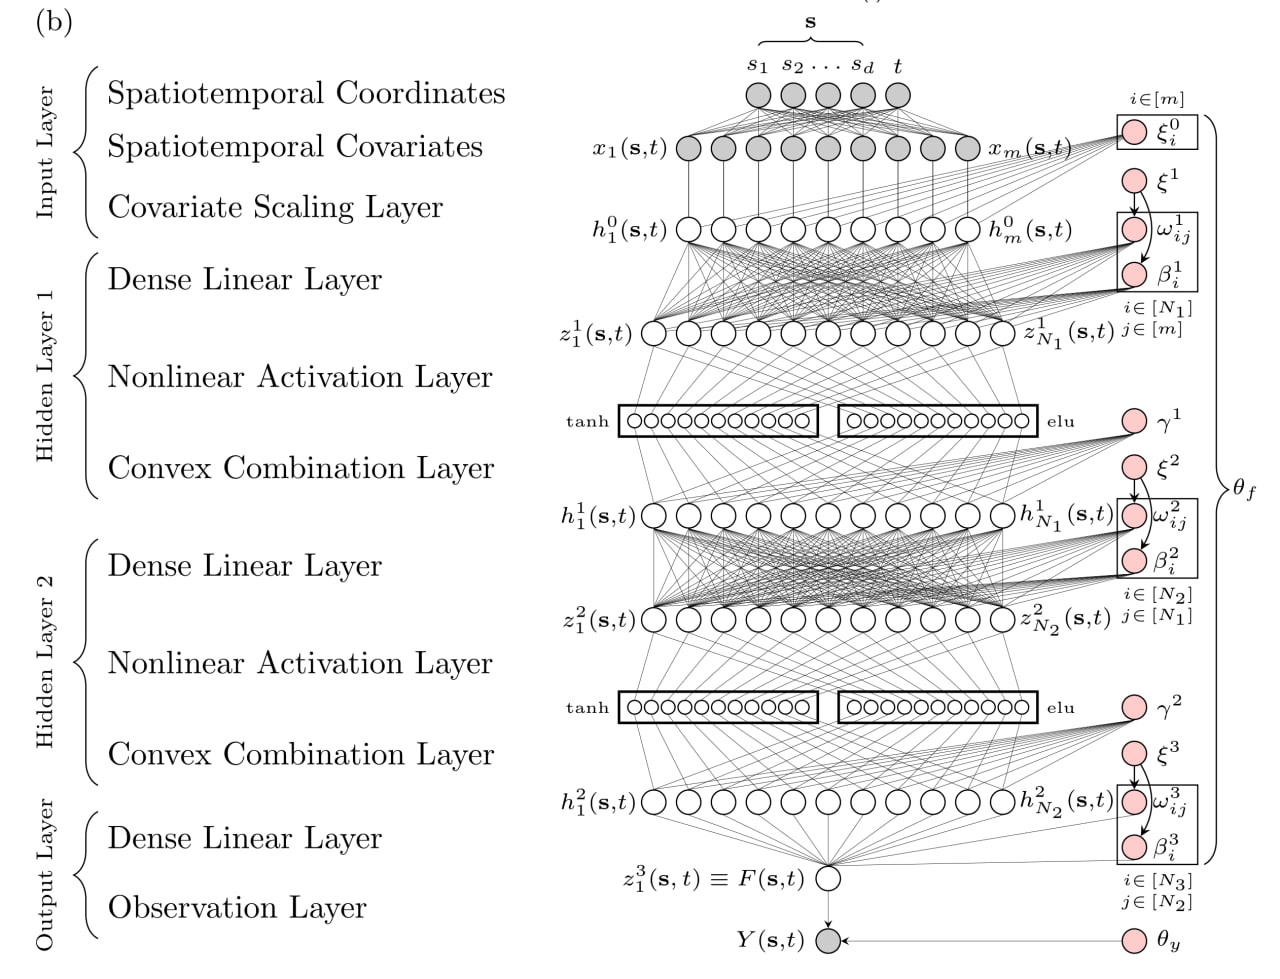
\includegraphics[width=0.95\textwidth]{images/06/bayesnf_architecture}
    \caption[BayesNF architecture]{Architecture of a Bayesian Neural
    Field with two hidden layers, after Saad et al.~\cite{saad2024bnf}}
    \label{fig:bayesnf-architecture}
\end{figure}

\subsubsection*{Covariate scaling layer}

This layer applies an element-wise rescaling
$\tilde{x}_i = e^{\xi_i}\,x_i$ with a learnable scale factor $e^{\xi_i}$
per covariate~\cite{saad2024bnf}. The appropriate scale is therefore
absorbed into the model parameters rather than requiring manual
standardisation of inputs, which otherwise heavily influences the
learning dynamics.

\subsubsection*{Fourier feature layer}

Plain multilayer perceptrons exhibit a \emph{spectral bias}: in the
neural tangent kernel limit they correspond to kernels with a rapid
frequency falloff, and therefore struggle to learn high-frequency
content from raw coordinates~\cite{tancik2020fourier}. Tancik et al.\
demonstrate that prepending a Fourier feature mapping transforms the
effective kernel into a stationary one with a tunable bandwidth, which
allows a multilayer perceptron to learn high-frequency functions in
low-dimensional problem domains~\cite{tancik2020fourier}. BayesNF adopts
this idea: each spatial axis $s_i$ is lifted into a bank of harmonics
\begin{equation}
  \phi_{s_i}(s_i) \;=\;
    \bigl\{\cos(2\pi\, 2^h\, s_i),\;\sin(2\pi\, 2^h\, s_i)\bigr\}_{h\in\mathcal{H}_{s_i}},
  \label{eq:bnf-spatial-fourier}
\end{equation}
and an analogous seasonal encoding is applied to the time axis with
period lengths chosen for the data's natural calendar
units~\cite{saad2024bnf}. This construction is theoretically justified
by the random Fourier feature framework of Rahimi and
Recht~\cite{rahimi2007rff}: Bochner's theorem characterises every
continuous shift-invariant positive-definite kernel on $\mathbb{R}^d$
as the Fourier transform of a non-negative measure, and the inner
product of two random Fourier feature vectors gives an unbiased Monte
Carlo estimate of that kernel. Combining Fourier features with a deep
neural prior therefore yields an expressive, data-driven covariance
structure rather than a pre-specified one. The empirical importance of
this layer is confirmed by an ablation study in Saad et al., which
reports substantial increases in RMSE, MAE, and MIS across most
benchmarks when the spatial Fourier features are
removed~\cite{saad2024bnf}.

\subsubsection*{Hidden layers with mixed activations}

The Fourier-encoded inputs are passed through $L+1 \geq 1$ dense hidden
layers. The non-linearity at each layer is a learnable softmax-weighted
convex combination of a small set of primitive activations, typically
$\{\tanh, \mathrm{relu}, \mathrm{elu}\}$~\cite{saad2024bnf}. This design
draws on the theory of expressive priors in Bayesian neural networks. In
the infinite-width limit, a Bayesian neural network converges to a
Gaussian process whose kernel is determined by the choice of activation
function: Pearce et al.\ show that swapping activation functions
effectively swaps the parametric form of the kernel, and that combining
several activations within an architecture induces a corresponding
combination of the underlying kernels~\cite{pearce2020expressive}.
BayesNF specialises this construction to a learnable softmax-weighted
convex combination, which Saad et al.\ motivate as a way to automate the
discovery of the covariance structure of the field, given that
activation functions correspond directly to the covariance of random
functions defined by Bayesian neural networks~\cite{saad2024bnf}.
Epistemic uncertainty is expressed by placing prior distributions over
all learnable parameters of the network, including the covariate scale
factors, the connection weights and biases, and the convex combination
coefficients.

\subsubsection*{Observation layer}

The hidden stack returns a real-valued latent field $F(\mathbf{s},t)$,
whereas the observable $Y(\mathbf{s},t)$ in this work is a non-negative
precipitation amount with a point mass at zero and a heavy right tail.
The \textbf{observation layer} maps $F(\mathbf{s},t)$ together with a
small set of global noise parameters $\Theta_y$ to a parametric
distribution $\mathrm{Dist}(\cdot;\,F(\mathbf{s},t),\Theta_y)$ on the
support of $Y$. The layer has two roles. First, it encodes the
\emph{aleatoric} uncertainty of the data-generating process: even if
$F$ were known exactly, $Y$ would remain random, and $\mathrm{Dist}$
specifies how. Second, it maps the unconstrained network output onto
the correct support, whether non-negative reals, non-negative integers,
or a zero-inflated mixture of the two, through a link function tied to
the choice of family. The choice of $\mathrm{Dist}$ therefore encodes
prior knowledge about the marginal distribution of the target and
dictates both the discretisation requirements on $Y$ and the form of
the predictive distribution at inference time.

The reference \texttt{google/bayesnf} implementation ships three
families~\cite{bayesnfRepo}:
\begin{description}
  \item[\texttt{NORMAL}] $Y(\mathbf{s},t) \sim
    \mathcal{N}\!\bigl(F(\mathbf{s},t),\,\sigma^{2}\bigr)$
    with a single learned noise scale~$\sigma$. Used for
    approximately Gaussian, real-valued targets.
  \item[\texttt{NB}] negative binomial with mean
    $\mu(\mathbf{s},t)=\mathrm{softplus}(F(\mathbf{s},t))$ and a learned
    dispersion shape~$\alpha$, so that
    $\mathrm{Var}[Y] = \mu + \alpha\,\mu^{2}$~\cite{bayesnfRepo}.
    Used for non-negative integer counts with overdispersion.
  \item[\texttt{ZINB}] zero-inflated negative binomial combining a
    Bernoulli mass at zero with probability $\pi_{0}$ and the
    negative binomial above with probability $1-\pi_{0}$, where $\pi_{0}$
    is a global learned parameter shared across all
    $(\mathbf{s},t)$~\cite{bayesnfRepo}.
\end{description}
\texttt{ZINB} matches daily precipitation: the marginal distribution
contains both a dry-day spike at zero and a heavy-tailed continuous
component. It is the family used in Chapter~\ref{ch:bayesnf}. Because
\texttt{NB} and \texttt{ZINB} are defined on $\mathbb{N}_{0}$, the
continuous precipitation amount must be discretised before training;
the discretisation and the inverse mapping used at prediction time are
described in Chapter~\ref{ch:bayesnf}.

\subsection{Inputs and hyperparameters}
\label{sec:theory-bayesnf-data}

Because the network absorbs the role of variogram model, transform,
neighbourhood index, and wet-dry decomposition, the data interface of
BayesNF is minimal: the required input is a long-table data frame in
which each row corresponds to one observation and stores its longitude,
latitude, time stamp, the target value $y$, and any number of static or
time-varying covariates~\cite{bayesnfRepo}. The remaining design choices
reduce to four hyperparameters: the harmonic sets $\mathcal{H}_{s_i}$ and
seasonal period set, which encode prior
expectations about spatial detail and temporal seasonality; the depth and
width of the dense backbone; the observation family $\mathrm{Dist}$
matched to the target distribution; and the posterior inference
algorithm, discussed next.

\subsection{Inference}
\label{sec:theory-bayesnf-inference}

\begin{sloppypar}
The posterior over network parameters is analytically
intractable~\cite{saad2024bnf}, so BayesNF relies on approximate inference.
Two scalable schemes are used: stochastic maximum-a-posteriori (MAP)
estimation, which returns a single parameter mode per random seed and is
fast but loses much of the posterior uncertainty; and mean-field
stochastic variational inference (VI), which fits a factorised
posterior and recovers wider predictive distributions at additional
computational cost.
\end{sloppypar}

\medskip\noindent
BayesNF is therefore the third candidate evaluated experimentally in
this thesis, alongside Ordinary Kriging (Chapter~\ref{ch:kriging}) and
gradient-boosted trees (Chapter~\ref{ch:gbm}).

%=============================================================================
\section{Evaluation metrics}
\label{sec:theory-metrics}
\label{sec:theory-crps}
%=============================================================================

All three interpolation methods in this thesis are evaluated using two metrics
applied consistently across Chapters~\ref{ch:kriging}--\ref{ch:comparison}.

\textbf{Mean Absolute Error (MAE)} measures point prediction accuracy as the
average absolute difference between predicted and observed precipitation
\cite{willmott2005mae}:
\begin{equation}
  \mathrm{MAE} = \frac{1}{n}\sum_{i=1}^{n}\bigl|\hat{Z}_i - Z_i\bigr|,
  \label{eq:mae}
\end{equation}
where $\hat{Z}_i$ and $Z_i$ are the predicted and observed values in
millimetres. MAE is expressed in the same physical units as precipitation and
is straightforward to interpret: a MAE of 1~mm means predictions are off by
1~mm on average. It evaluates only the point estimate, however, and says
nothing about the quality of the predicted uncertainty.

To assess the \textbf{full predictive distribution} of a probabilistic model,
the \textbf{Continuous Ranked Probability Score (CRPS)} is used
\cite{gneiting2007strictly}:
\begin{equation}
  \mathrm{CRPS}(F,\, y)
    = \int_{-\infty}^{\infty}
      \bigl(F(z) - \mathbf{1}\{z \ge y\}\bigr)^{2}\,\mathrm{d}z,
  \label{eq:crps}
\end{equation}
where $F$ is the predicted cumulative distribution function and $y$ is the
observation.  Intuitively, CRPS measures the integrated squared distance
between the forecast CDF and the ``perfect'' CDF, a unit step function at the
observed value.  A lower CRPS indicates a predictive distribution that is both
well-calibrated (centred on the truth) and sharp (concentrated, not
unnecessarily wide).

\begin{figure}[H]
    \centering
    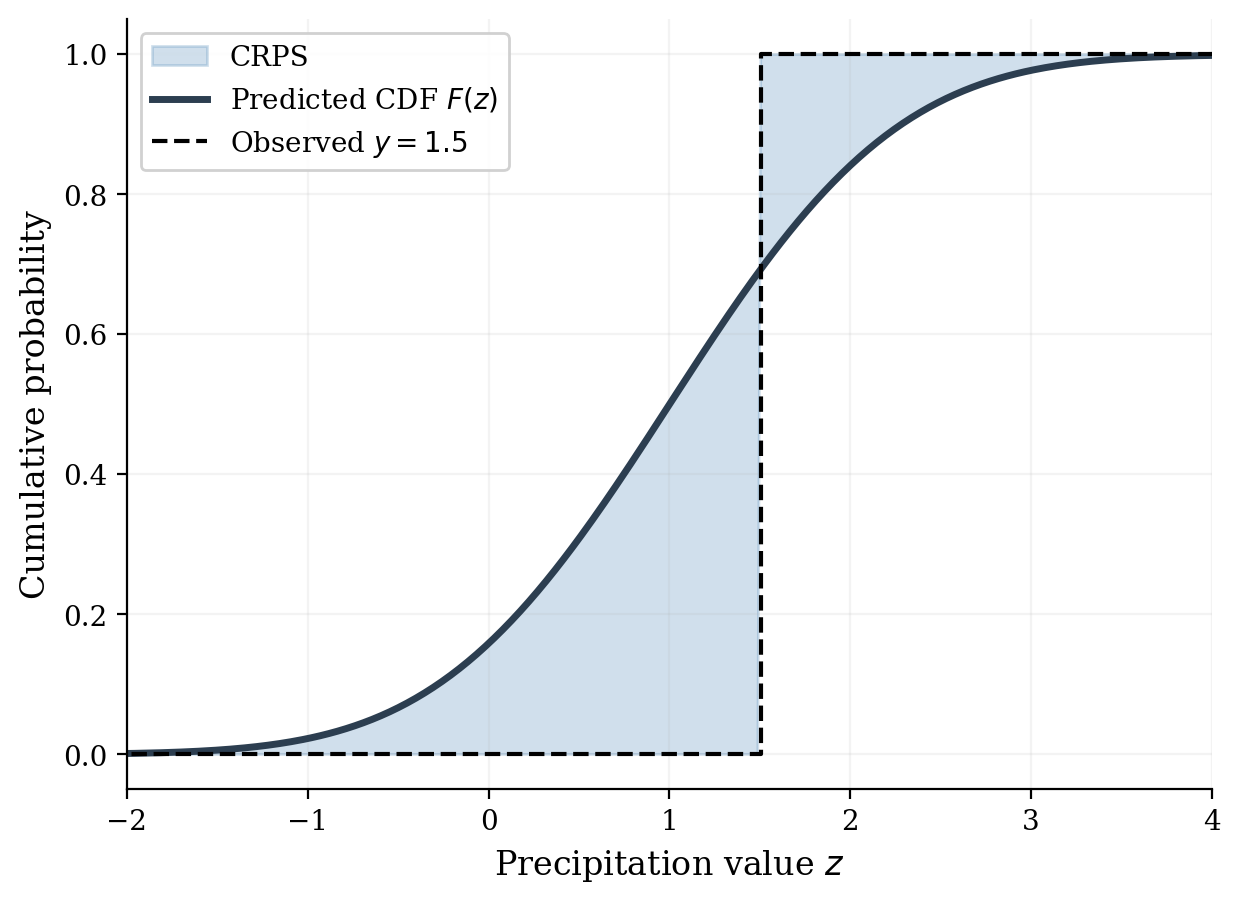
\includegraphics[width=0.85\textwidth]{images/02/crps_diagram}
    \caption[Geometric interpretation of CRPS]{Geometric interpretation of CRPS: the shaded area between the predicted CDF $F(z)$ and the step function at observed value~$y$; redrawn after Gneiting and Raftery~\cite{gneiting2007strictly}}
    \label{fig:crps-diagram}
\end{figure}

In practice the predictive distribution $F$ is rarely available in closed
form. Both the kriging and the gradient-boosting models in this work
represent $F$ by an ensemble of $M$ samples
$x_{1},\dots,x_{M}\sim F$ (for kriging, these are Monte-Carlo
back-transforms of Gaussian draws; see Equation~\eqref{eq:mc-backtrafo}). The
naive plug-in estimator that replaces $F$ by the empirical CDF of the
ensemble is biased downward at finite $M$ and only recovers the true CRPS in
the limit $M\!\to\!\infty$.  To obtain an unbiased estimate at any ensemble
size, the \textbf{fair CRPS estimator} of Ferro~\cite{ferro2014fair} is used:
\begin{equation}
  \widehat{\mathrm{CRPS}}_{\text{fair}}(x_{1:M},\,y)
    = \frac{1}{M}\sum_{m=1}^{M}\bigl|x_{m}-y\bigr|
    - \frac{1}{2\,M(M-1)}\sum_{m=1}^{M}\sum_{m'=1}^{M}\bigl|x_{m}-x_{m'}\bigr|.
  \label{eq:fair-crps}
\end{equation}
The first term measures the average distance of ensemble members to the
observation; the second is a finite-sample correction that subtracts the
ensemble's internal spread.  This estimator is unbiased for the population
CRPS under the standard assumption that ensemble members are exchangeable
draws from $F$, and it is the form actually computed in
Chapters~\ref{ch:kriging}--\ref{ch:comparison}.

CRPS is a \textbf{strictly proper scoring rule} for distributions with
finite first moment \cite{gneiting2007strictly}: its expectation is
minimised if and only if the predicted distribution equals the true
data-generating distribution.  This
means CRPS simultaneously penalises \emph{overconfidence} (intervals too narrow
that frequently miss the observation) and \emph{diffidence} (intervals too wide
that carry no useful information).  Unlike mean absolute error, CRPS therefore
provides a single number that rewards honest uncertainty quantification.

The root-mean-square error (RMSE), common in climatology, is \emph{not} used
in this work.  RMSE implicitly assumes Gaussian residuals, an assumption incompatible
with daily precipitation: the variable is non-negative, zero-inflated, and
heavy-tailed, so RMSE under-penalises rare extreme events and ignores the
large probability mass at zero \cite{hunt2025stop}.  CRPS, by contrast,
is a proper scoring rule that evaluates the full predictive distribution
without parametric assumptions, making it better suited to precipitation data.


\chapter{Data and Study Area}
\label{ch:data}

\section{Study Area}

The study area covers northern and central Germany with adjacent border regions
of the Czech Republic and Poland, bounded by longitudes $9.4^\circ$--$15.9^\circ$\,E
and latitudes $50.0^\circ$--$53.8^\circ$\,N.
This region spans approximately 430 km west to east and 440 km north to south,
encompassing the German federal states of Schleswig-Holstein, Hamburg, Bremen,
Mecklenburg-Vorpommern, Brandenburg, Berlin, Lower Saxony, Saxony-Anhalt, and
the northern parts of Saxony and Thuringia, as well as adjacent areas of
northern Bohemia (Czech Republic) and western Poland. The rectangular bounding
box intentionally extends beyond the German border to ensure adequate station
coverage for interpolation near boundary regions, avoiding edge effects that
would otherwise degrade prediction quality at the periphery of the domain.

The northern and central parts of the domain are dominated by the North German
Plain (\textit{Norddeutsche Tiefebene}), a broad lowland formed by
Pleistocene glaciation, with elevations predominantly below 200~m above sea
level.  The northern boundary meets the Baltic Sea coast, introducing maritime
influences on the precipitation regime.  Towards the south and southeast,
the terrain rises sharply: the Harz Mountains at the centre of the domain and
a continuous belt of uplands along the borders of southeastern Germany,
northern Bohemia, and southwestern Poland reach elevations above 1\,000~m;
these uplands include the Erzgebirge (Ore Mountains), the Thuringian Forest,
and the western Sudetes.

\textbf{Orographic lifting} \cite{daly1994prism} produces enhanced
precipitation on the windward (north-western) slopes of the southern
mountain ranges, while the lee sides and interior basins receive
substantially less, a phenomenon known as the \textbf{rain shadow} effect.
As a result, annual precipitation totals range from roughly
500--600~mm on the sheltered lowlands to over 1\,000~mm in the highest
parts of the Harz and the Erzgebirge, as computed from the ReKIS station
network (Table~\ref{tab:elevation_means}).
This large-scale orographic gradient makes the region a challenging
testbed for spatial interpolation methods.

All spatial computations use the ETRS89-LAEA coordinate reference system
(EPSG:3035), an equal-area projection appropriate for European studies, ensuring
that areas are preserved accurately across the domain, with distance
distortion remaining below 1\% at this regional scale.
The primary prediction target is a regular 1~km $\times$ 1~km grid
containing 189{,}648 cells; the best-performing method is additionally
applied at coarser spatial resolutions.
Table~\ref{tab:terrain-zones} shows how these cells are distributed across
three elevation zones: about 71\% of the domain lies on the lowland plain,
while about 7.5\% falls in mountainous terrain above 500~m.

\begin{table}[ht]
  \centering
  \caption{Distribution of the 1~km prediction grid cells across terrain zones}
  \label{tab:terrain-zones}
  \begin{tabular}{lccc}
    \toprule
    Terrain zone & Elevation range & Grid cells & Share \\
    \midrule
    Plains    & 0--250~m   & 133{,}970 & 70.6\% \\
    Hills     & 250--500~m &  41{,}411 & 21.8\% \\
    Mountains & $>$500~m   &  14{,}267 &  7.5\% \\
    \bottomrule
  \end{tabular}
\end{table}

\section{Observational Data: ReKIS Station Network}

\subsection{Network Description}

Daily precipitation measurements were obtained from the Regionales
Klimainformationssystem (ReKIS), a regional climate information system
providing quality-controlled station data for northern and central Germany.%
\footnote{ReKIS is operated by the Saxon State Office for the
Environment, Agriculture and Geology (LfULG); see
\url{https://www.rekis.org}.}
The dataset covers 2{,}458 stations with continuous daily records spanning the
full analysis period from January~1,~1961 -- December~31,~2023, yielding
63 years of daily precipitation observations (Figure~\ref{fig:station}).
All stations report at least one wet day in every year of the record, indicating
uniform temporal coverage across the network with no station dropouts or
gaps in network density over time.
This long, spatially consistent record supports reliable estimation of
climatological monthly precipitation normals, which are used as a detrending
baseline in the interpolation pipeline (Section~\ref{sec:detrending}).

\begin{figure}[htbp]
    \centering
    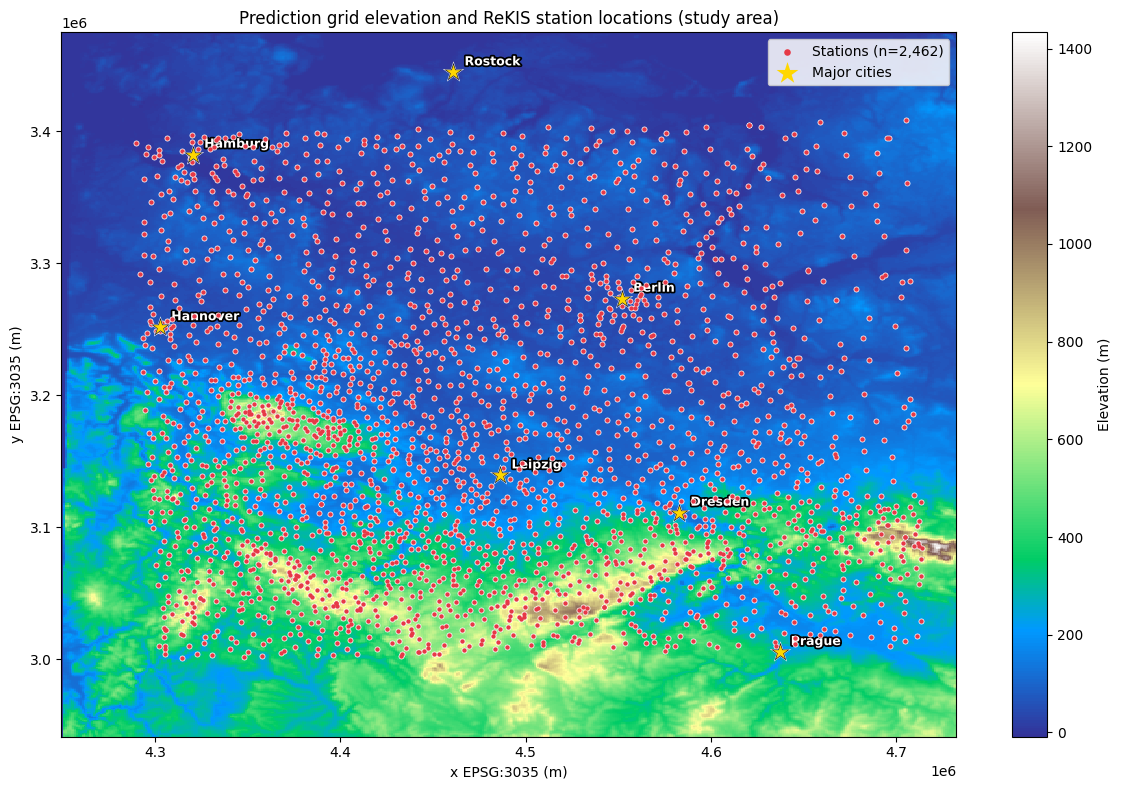
\includegraphics[width=0.95\textwidth]{images/03/station.png}
    \caption{The 2{,}458 ReKIS stations used in this study}
    \label{fig:station}
\end{figure}

\subsection{Quality Control}

A systematic quality control check was applied to the raw ReKIS data prior
to analysis.
Across all 56{,}650{,}620 station-day records, \textbf{no missing values and no
negative precipitation amounts} were detected, confirming the high completeness
of the network.

Two issues were identified and corrected.
First, 38 station IDs (predominantly cross-border Czech and Polish gauges)
appeared two or three times in the metadata catalogue with identical coordinates;
duplicates were removed, keeping one entry per station ID.
Second, four pairs of stations with distinct IDs shared identical geographic
coordinates, representing co-located gauges that would cause rank deficiency
in the kriging covariance matrix; these were merged by averaging their daily
records.
Together these corrections reduce the network from 2{,}462 to 2{,}458 unique
station locations.

\newpage
\section{Auxiliary Data}

\subsection{Digital Elevation Model}

\noindent\begin{minipage}[t]{0.50\textwidth}
\vspace{0pt}
Terrain elevation data were derived from the Copernicus Digital Elevation Model
\cite{copernicus_dem}, resampled to the same 1 km $\times$ 1 km grid as the
prediction target (Figure~\ref{fig:elevation}).
Elevation is used as a covariate when interpolating monthly precipitation
normals (the long-term mean monthly totals from the 1961--2023 station
record). Under the 3D thin-plate spline variant, these normals are
interpolated as a function of $(x, y, z_\text{elev})$, where $x$ and $y$
are the EPSG:3035 projected coordinates and $z_\text{elev}$ is terrain
elevation from the Copernicus DEM, rather than spatial coordinates alone.
This lets the model capture orographic enhancement of precipitation.
\end{minipage}
\hfill
\begin{minipage}[t]{0.47\textwidth}
\vspace{0pt}
\centering
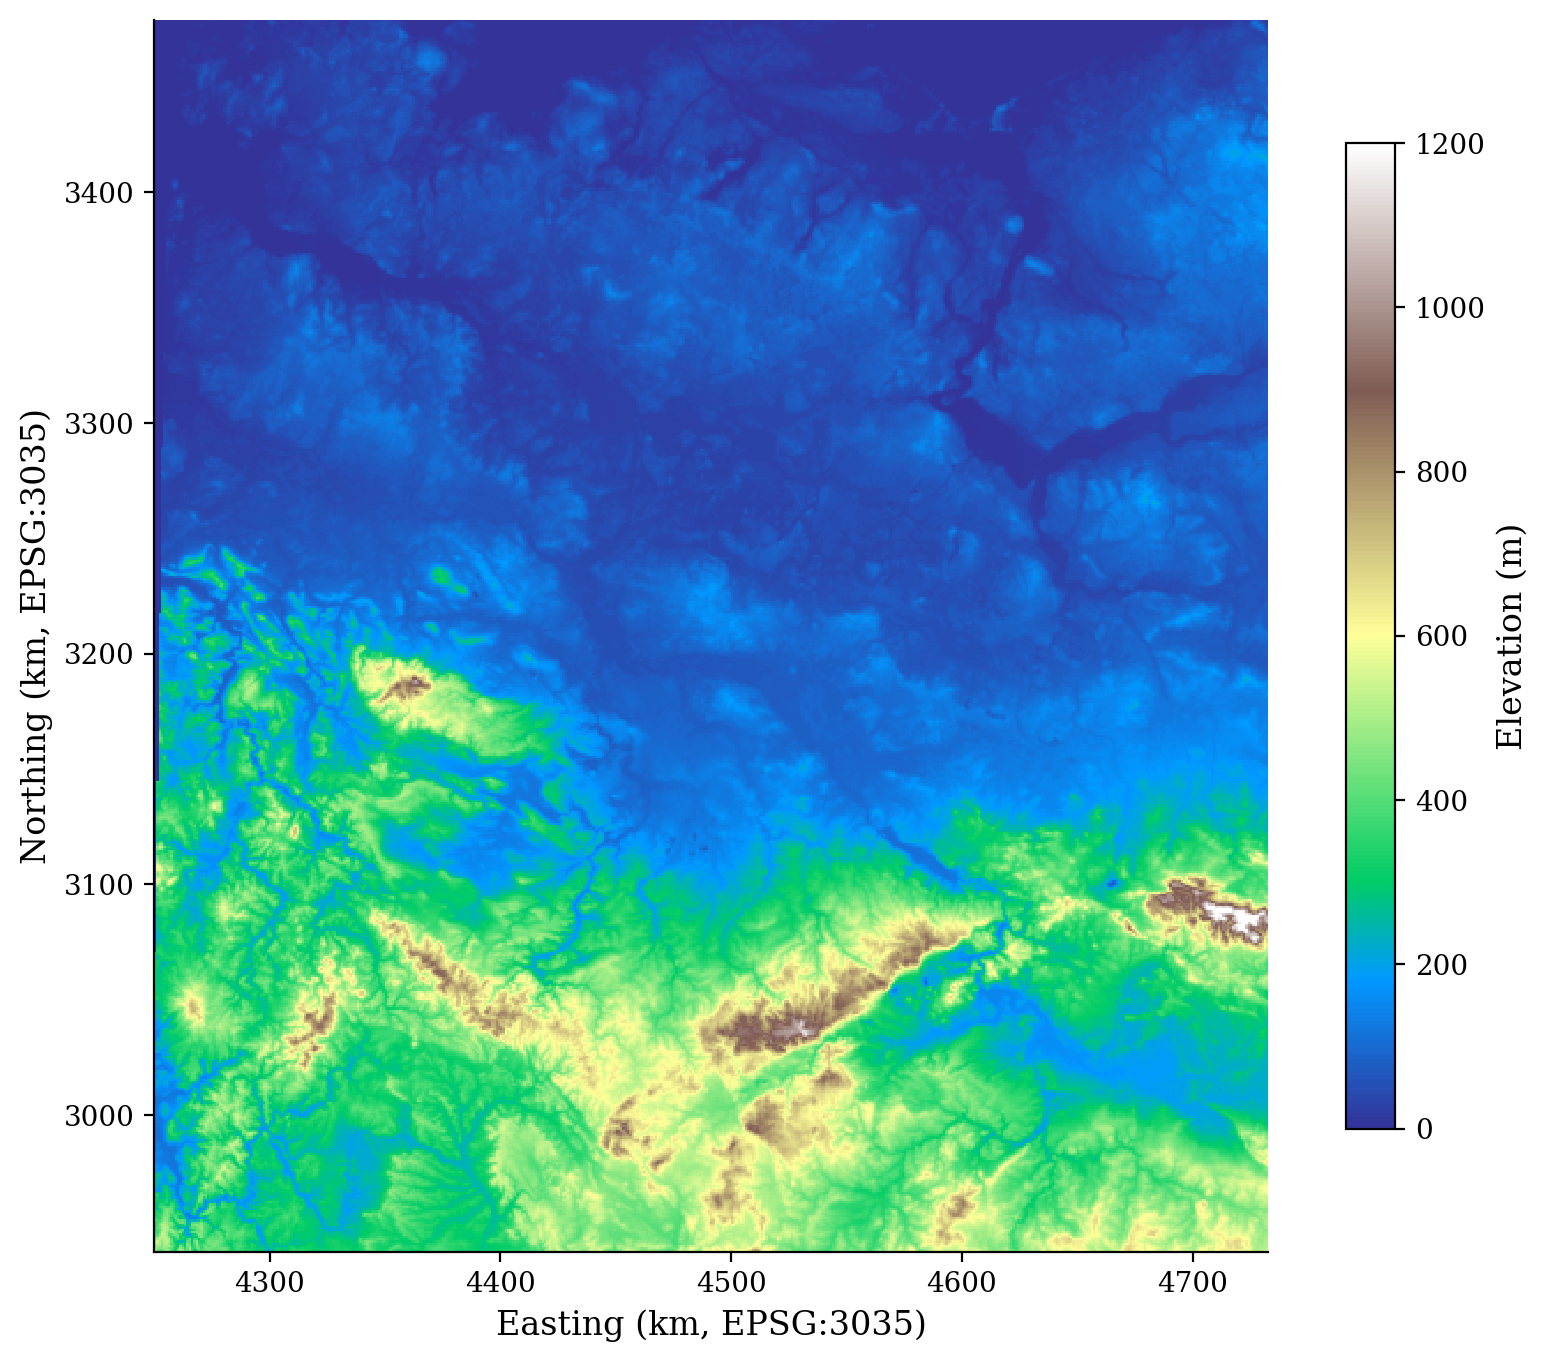
\includegraphics[width=\linewidth]{images/03/elevation.png}
\captionof{figure}{Elevation over the study area (Copernicus DEM, resampled to the 1~km grid)}
\label{fig:elevation}
\end{minipage}

\subsection{SoilGrids Auxiliary Variables}

\noindent\begin{minipage}{\textwidth}
Six soil properties from SoilGrids \cite{poggio2021soilgrids} are used
as auxiliary covariates for the gradient boosting model (LightGBM) and
the Bayes Neural Field: bulk density, clay content, sand content, silt
content, soil organic carbon, and volumetric water content at $-10$~kPa.
Each variable is averaged across the 0--30~cm depth range, yielding one
value per grid cell (Figure~\ref{fig:soilgrids}).

\vspace{0.8em}
\centering
\includegraphics[width=0.95\textwidth]{images/03/fig_soilgrids.png}
\captionof{figure}{SoilGrids auxiliary variables over the study area}
\label{fig:soilgrids}
\end{minipage}

\section{Statistical Properties of Daily Precipitation}
\label{sec:precip_statistics}

Daily precipitation data have several statistical properties that
directly complicate interpolation.
These properties drive the preprocessing and modelling choices
described in subsequent chapters.

\subsection{Zero-Inflation and Mixed Distribution}

Daily precipitation is intermittent: on any given day, a large fraction of
stations record no precipitation (dry days), while the remaining stations record
positive amounts.
This yields a mixed discrete-continuous distribution, a point mass at zero
combined with a right-skewed continuous component for positive values.
The proportion of dry days varies by season and location but typically exceeds
50\,\% across the study area \cite{haylock2008european}
(Figure~\ref{fig:precip_distribution}).

Standard interpolation methods designed for continuous Gaussian fields cannot
handle this mixed distribution.
The two-stage model described in Chapter~\ref{ch:kriging} addresses this
directly: a binary indicator stage separates wet from dry locations, and a
separate amount model is applied only to wet-day observations.

\begin{figure}[H]
    \centering
    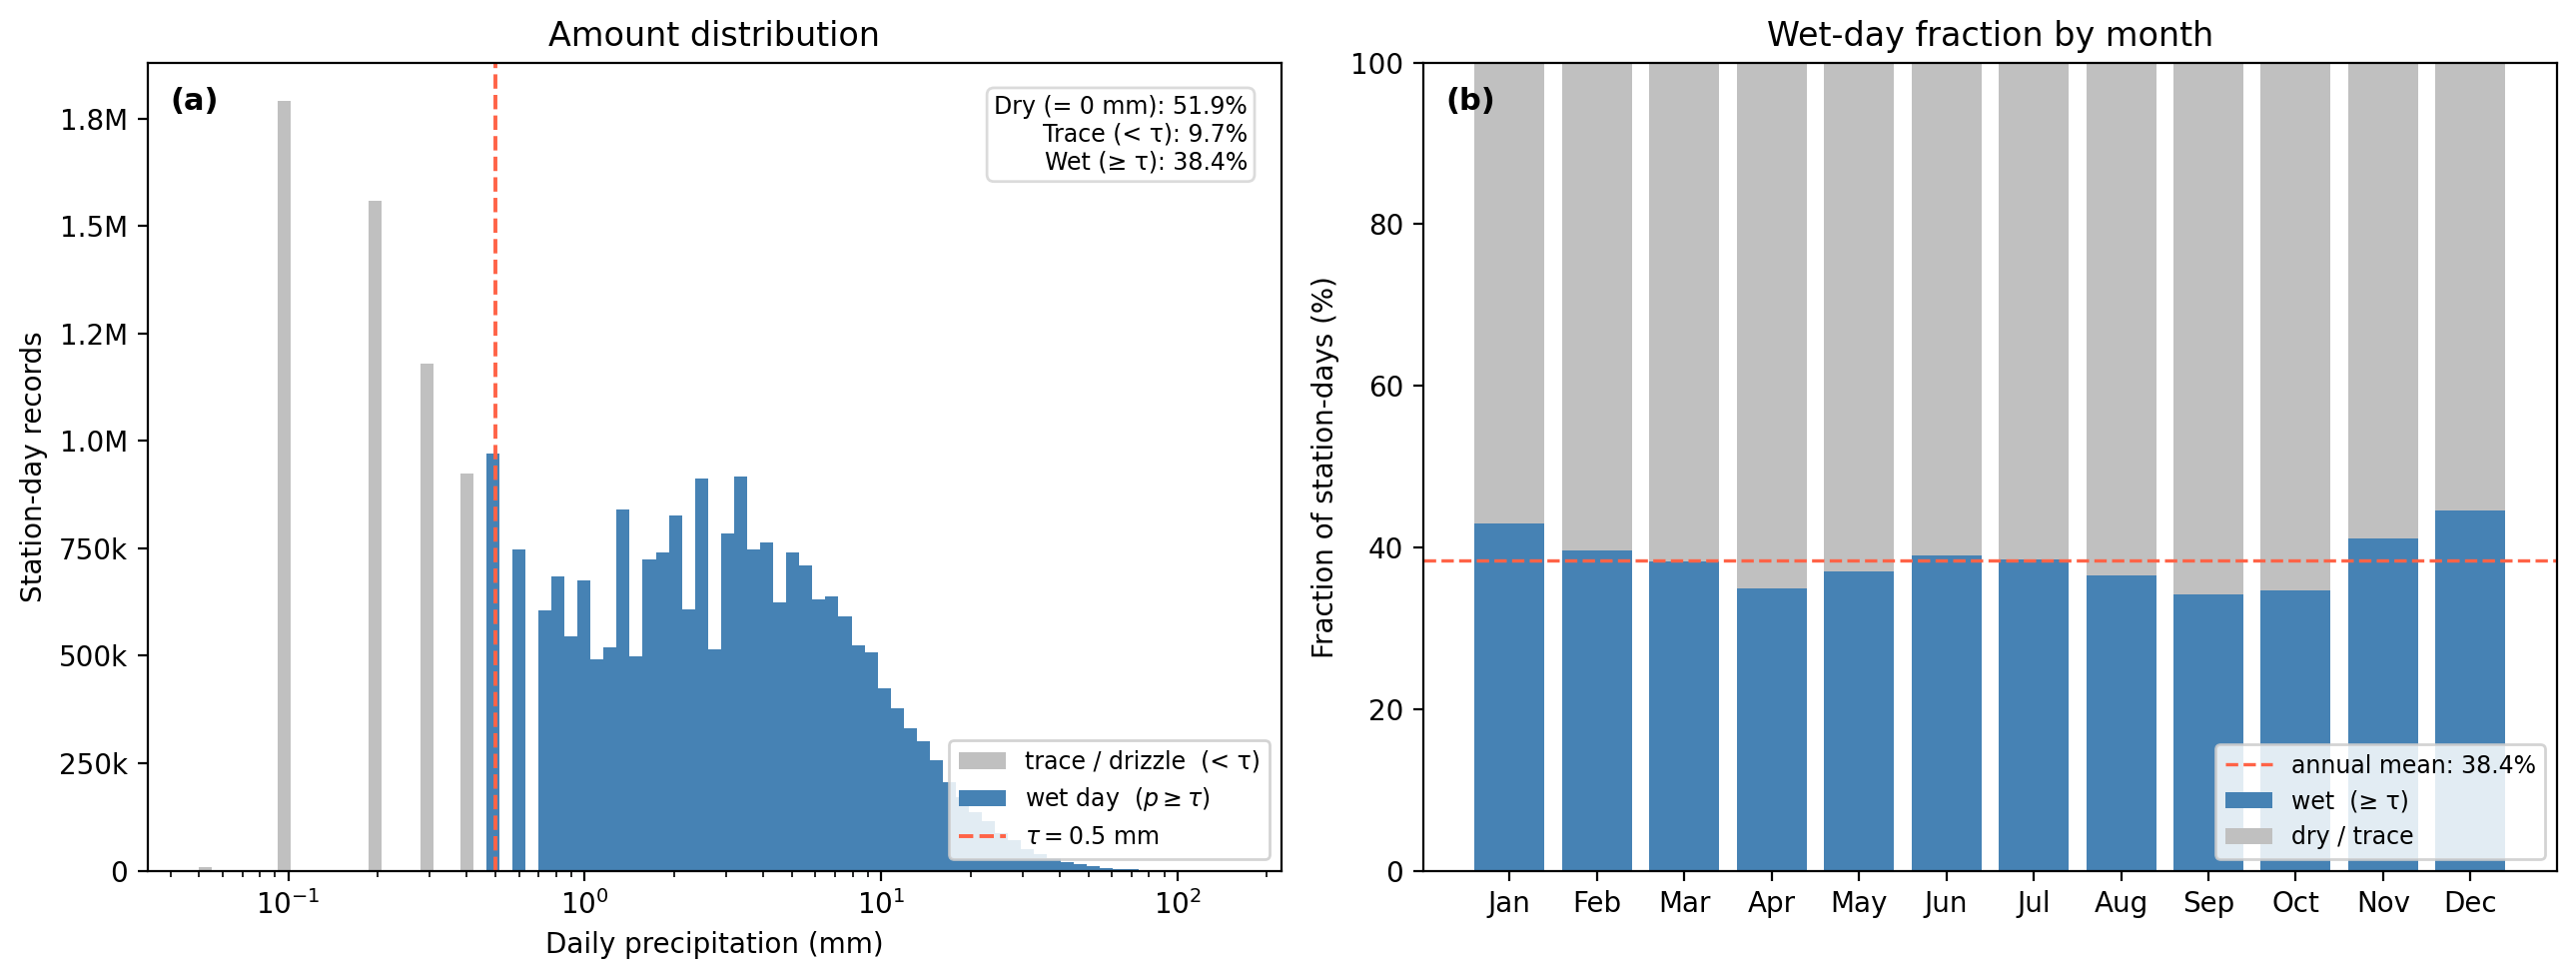
\includegraphics[width=0.95\textwidth]{images/03/fig_precip_distribution.png}
    \caption{Mixed discrete-continuous distribution of daily precipitation
    in the ReKIS network (1961--2023). Panel~(a): histogram of non-zero
    amounts on a log scale; dry-day fraction (51.9\,\%) and the wet-day
    threshold $\tau = 0.5$~mm are marked. Panel~(b): wet-day fraction
    by calendar month}
    \label{fig:precip_distribution}
\end{figure}

\subsection{Right-Skewed Amounts}

When conditioned on wet days, precipitation amounts follow a heavily
right-skewed distribution.
Rare but intense rainfall events contribute disproportionately to total
accumulation, producing a long upper tail \cite{hofstra2008comparison}
(Figure~\ref{fig:wetday_skewness}).
Climatological normalisation is applied before kriging to remove seasonal
non-stationarity and stabilise variance (Section~\ref{sec:detrending}).

\begin{figure}[H]
    \centering
    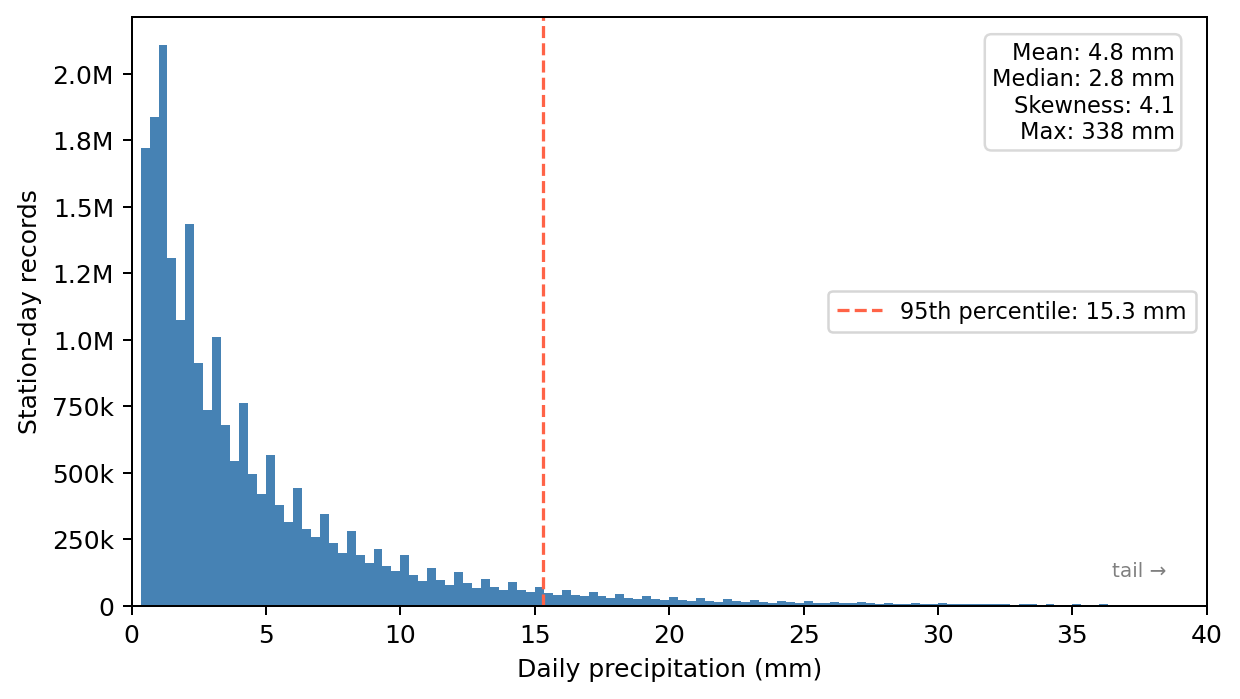
\includegraphics[width=0.7\textwidth]{images/03/fig_wetday_skewness.png}
    \caption{Distribution of wet-day precipitation amounts ($p \geq 0.5$~mm)
    across all ReKIS stations (1961--2023). The mean (4.8~mm) exceeds the
    median (2.8~mm) and the skewness is 4.1, confirming the heavy right tail.
    The 95th percentile (15.3~mm) is marked; extreme values extend to
    338~mm}
    \label{fig:wetday_skewness}
\end{figure}

\subsection{Seasonality and Non-Stationarity}

Precipitation in northern Germany shows strong seasonal variation.
Monthly mean values at the observational stations range from approximately 43.5~mm in
February to 74.7~mm in July (Figure~\ref{fig:monthly_means}).
This seasonal cycle is a large-scale non-stationarity that violates
the stationarity assumption of ordinary kriging.
Climatological normalisation in Chapter~\ref{ch:kriging} (Section~\ref{sec:detrending})
addresses it.

\begin{figure}[H]
    \centering
    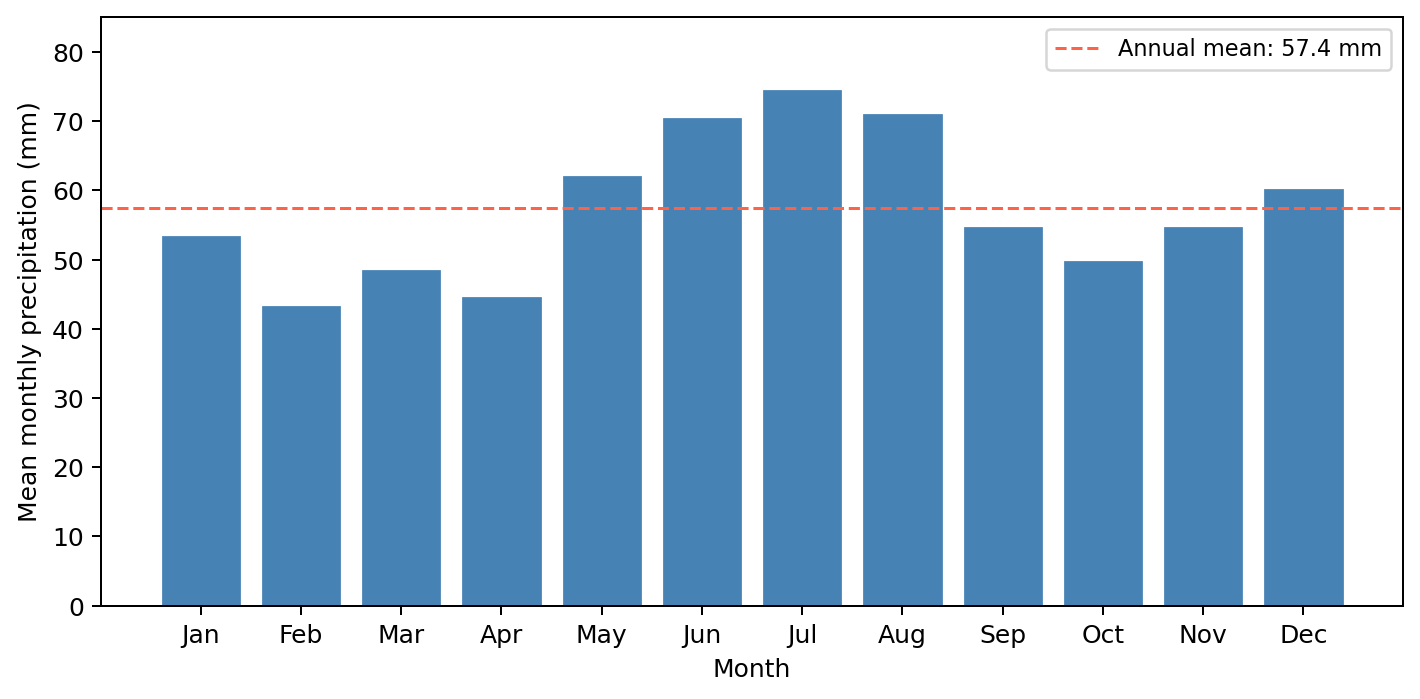
\includegraphics[width=0.8\textwidth]{images/03/fig_monthly_means.png}
    \caption{Mean monthly precipitation averaged over all ReKIS stations
    (1961--2023). The dashed line marks the annual mean of 57.4~mm}
    \label{fig:monthly_means}
\end{figure}

\subsection{Orographic Effects}

\begin{sloppypar}
Terrain elevation strongly affects precipitation, particularly
during winter months when frontal systems interact with topography
\cite{daly1994prism}.
In the study area, mean monthly precipitation at stations in the mountainous zone
(above 500~m) is approximately 85.9~mm, compared to 50.7~mm in the plains
(Table~\ref{tab:elevation_means}).
This orographic gradient reflects frontal systems interacting with
the mountainous terrain along the southern part of the domain.
\end{sloppypar}

\begin{table}[ht]
\centering
\caption{Mean monthly precipitation by terrain elevation zone (ReKIS, 1961--2023)}
\label{tab:elevation_means}
\begin{tabular}{lrrr}
\toprule
Elevation zone & N stations & Mean elev. (m) & Mean precip. (mm) \\
\midrule
Plains (0--250 m)    & 1{,}530 & 101 & 50.7 \\
Hills (250--500 m)   &    667  & 352 & 61.5 \\
Mountains (500+ m)   &    265  & 661 & 85.9 \\
\bottomrule
\end{tabular}
\end{table}

\chapter{Implementation of Ordinary Kriging}
\label{ch:kriging}

%=============================================================================
\section{Pipeline overview}
\label{sec:kriging-pipeline}
%=============================================================================

Ordinary Kriging is implemented as the geostatistical baseline against which
gradient boosting (Chapter~\ref{ch:gbm}) and Bayesian Neural Fields
(Chapter~\ref{ch:bayesnf}) are evaluated. The pipeline follows the two-stage
decomposition $Z = I \cdot A$ from
Section~\ref{sec:kriging-indicator}: a binary indicator stage produces a
wet/dry classification, and an amount stage predicts precipitation magnitude
on cells classified as wet. The amount stage operates in three steps:
climatological normalisation (Section~\ref{sec:detrending}) removes seasonal
and orographic non-stationarity, Ordinary Kriging is solved on the normalised
values, and a Monte Carlo back-transformation maps the prediction back to
physical millimetres. Cross-validation uses the 5-fold station split shared
with the gradient boosting and BayesNF chapters on 1{,}966 training stations,
with 492 holdout stations reserved for the final test.

\begin{figure}[ht]
    \centering
    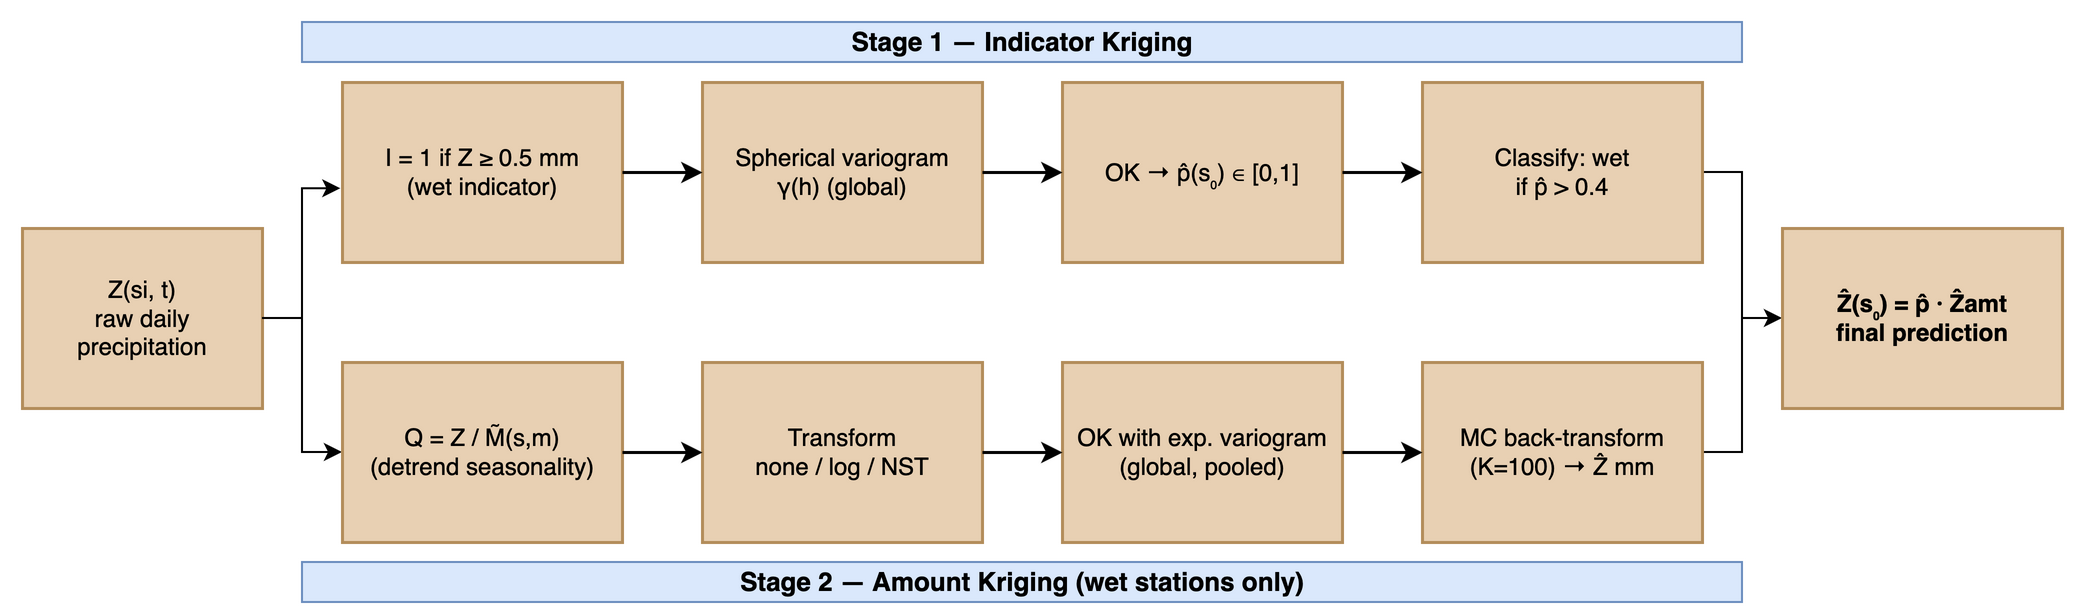
\includegraphics[width=0.95\textwidth]{images/04/two_stage_architecture}
    \caption{Two-stage kriging pipeline. Stage~1 produces a binary
    wet/dry mask via indicator kriging; Stage~2 interpolates the
    climatological ratio at wet cells and back-transforms to physical
    millimetres}
    \label{fig:two-stage-architecture}
\end{figure}

%=============================================================================
\section{Stage~1: indicator kriging}
\label{sec:kriging-indicator-impl}
%=============================================================================

Stage~1 implements the indicator decision of
Equation~\eqref{eq:indicator-decision} using the \texttt{PyKrige} Python
library. Each station observation is converted to a wet-day indicator
$I = \mathbf{1}[Z \geq \tau]$ with threshold $\tau = 0{.}5$~mm — the
standard E-OBS value, chosen above the typical $0{.}1$--$0{.}2$~mm gauge
measurement accuracy \cite{haylock2008european}.
Following Hofstra et al.~\cite{hofstra2008comparison}, a \textbf{spherical}
variogram is used for the indicator field
(Figure~\ref{fig:indicator-variogram}). The model is fitted globally by
pooling empirical indicator semi-variance across all wet days of the
1961--2023 record, excluding days on which all stations are wet or all are
dry (the indicator has zero variance in those cases). Ordinary Kriging on
the binary inputs produces, at every grid cell, the wet-day probability
$\hat{p}(\mathbf{s}_0)$. The decision threshold $p^{\star} = 0{.}4$
\cite{hofstra2008comparison} converts this probability into a binary
classification: cells with $\hat{p} > 0{.}4$ are passed to Stage~2, the
remaining cells are set to zero precipitation.

\begin{figure}[H]
    \centering
    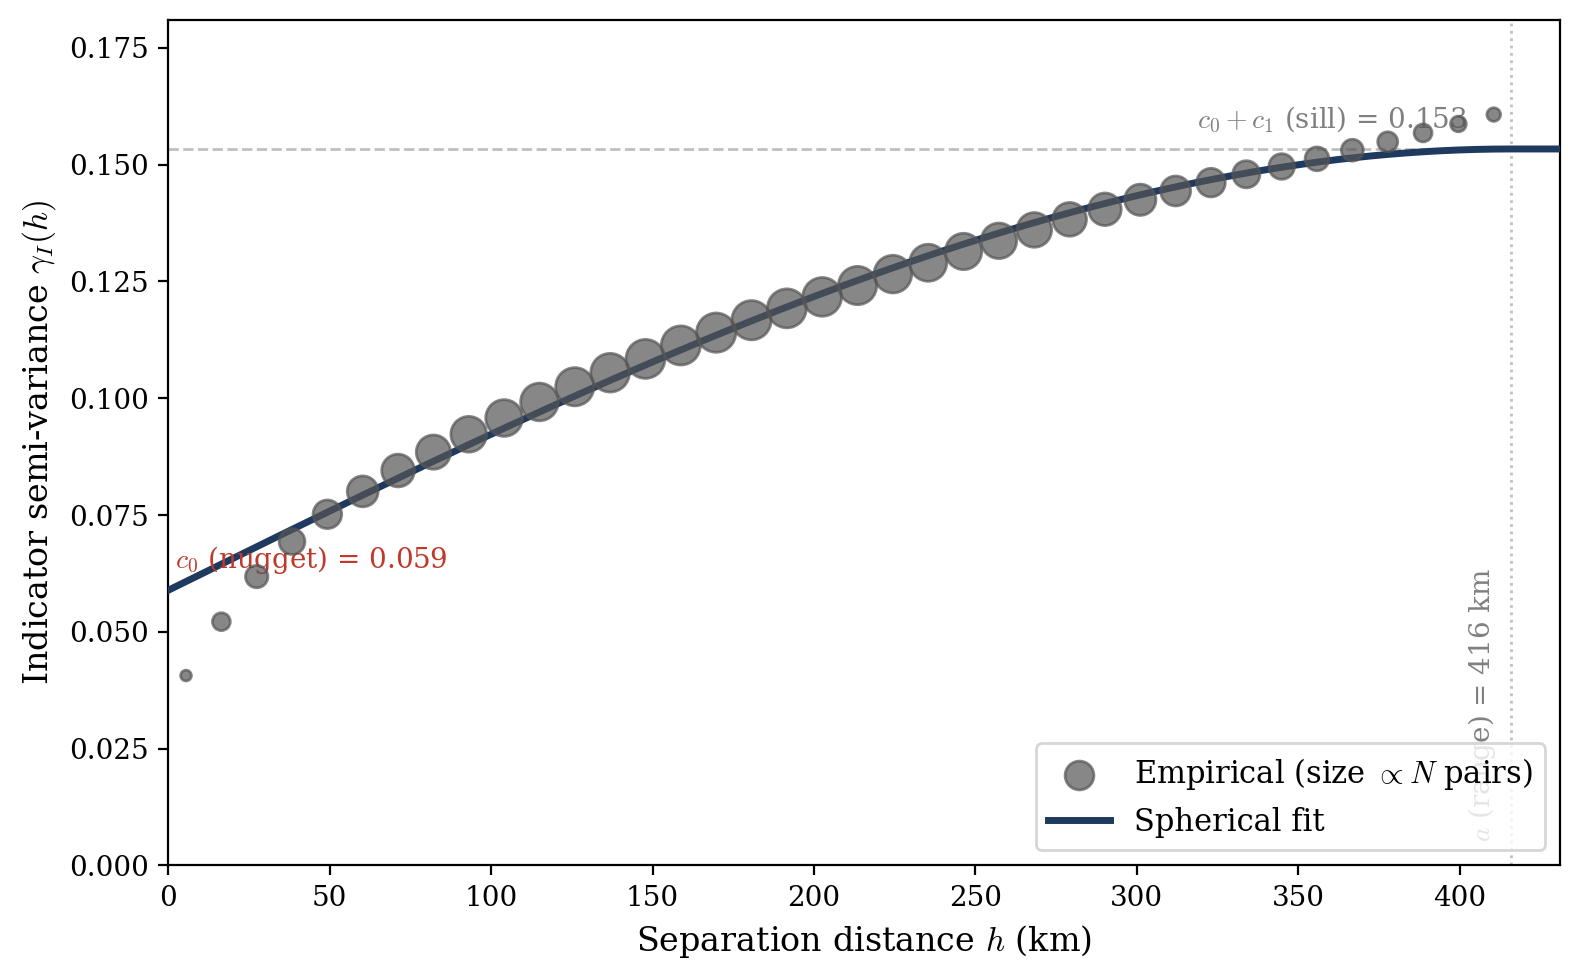
\includegraphics[width=0.85\textwidth]{images/04/indicator_variogram}
    \caption{Global indicator semi-variogram pooled across all wet days of
    the 1961--2023 record (empirical points, marker size proportional to
    the number of station pairs in each lag bin), and the fitted spherical
    model}
    \label{fig:indicator-variogram}
\end{figure}

\begin{figure}[H]
    \centering
    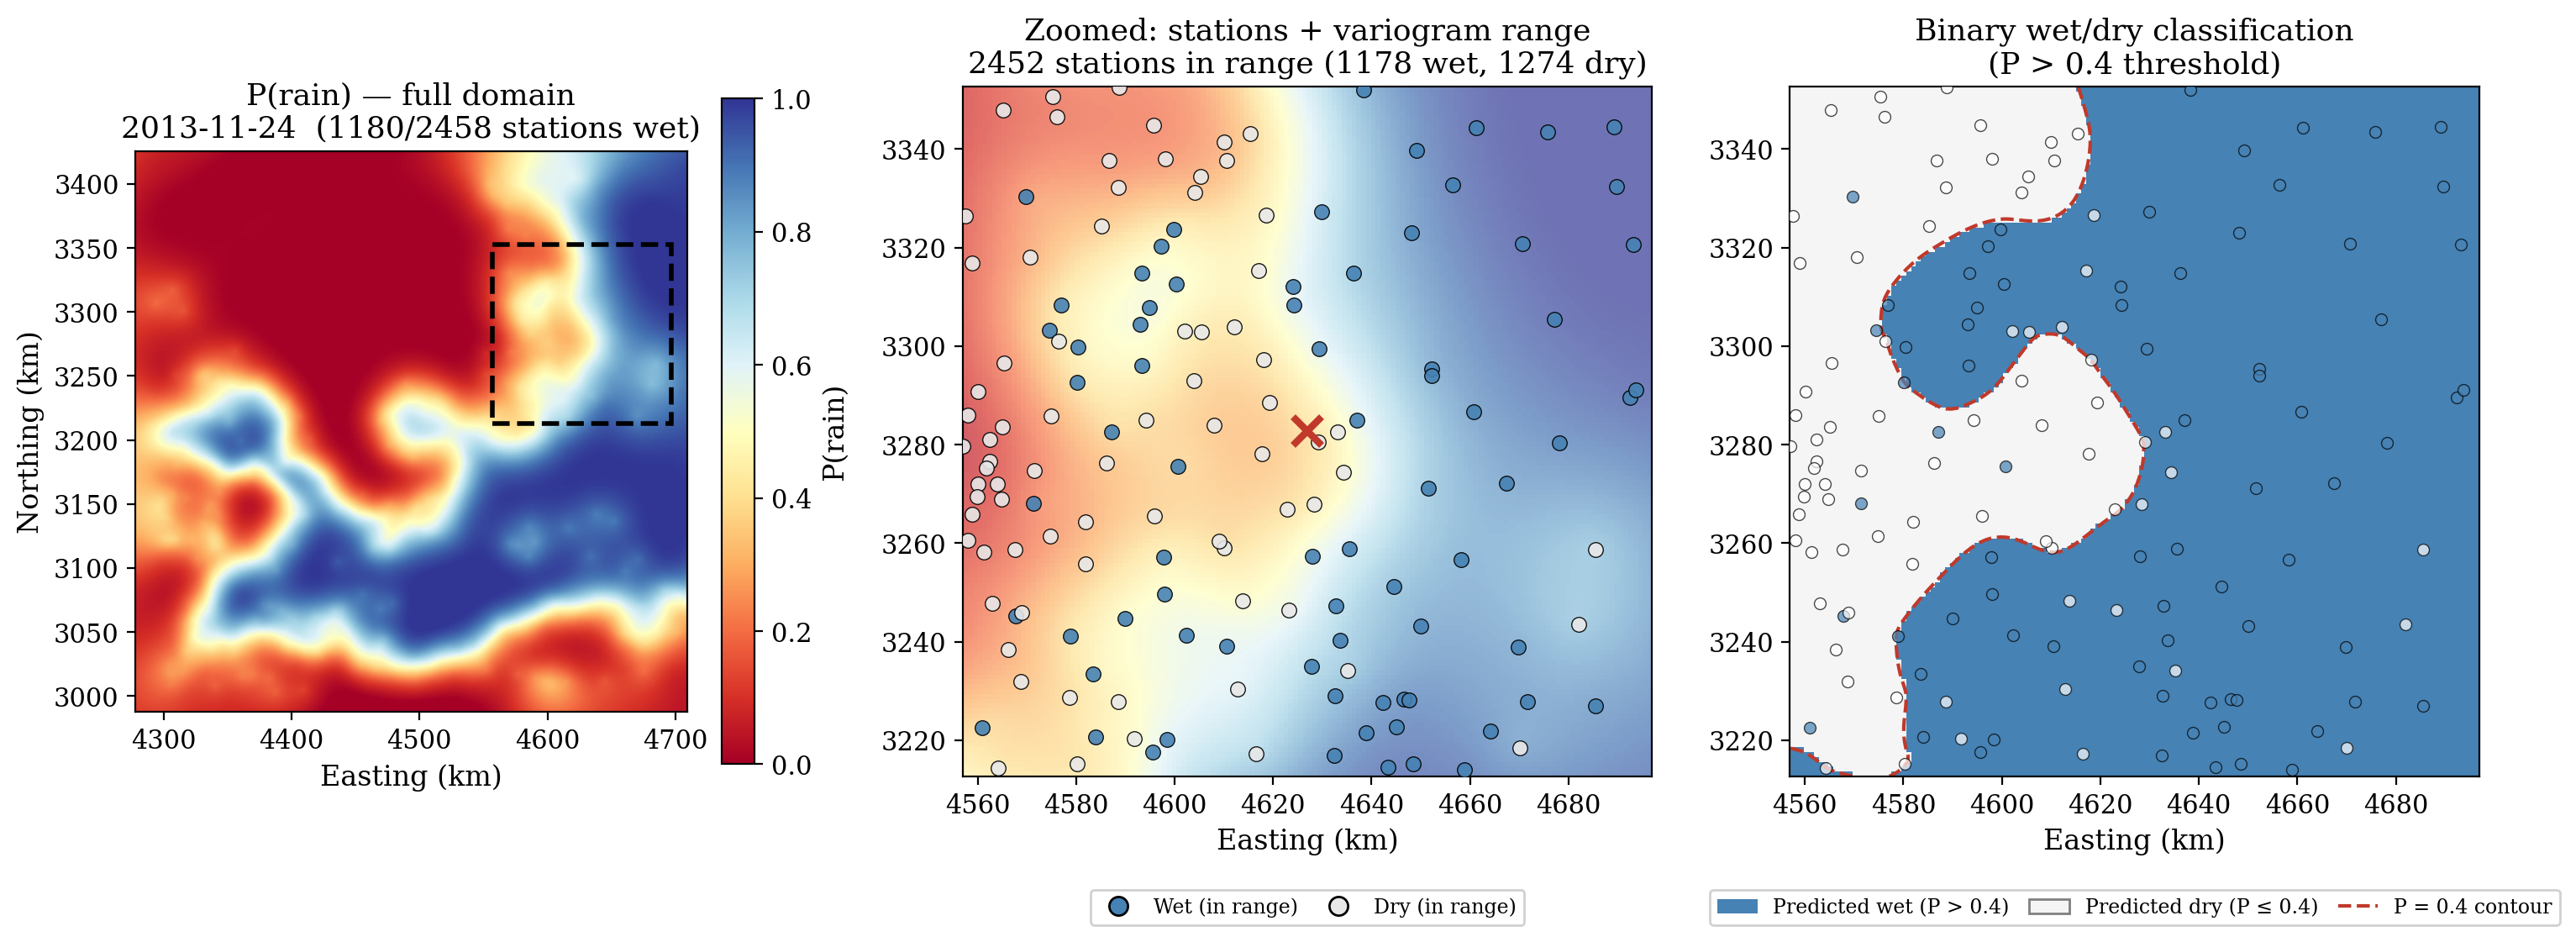
\includegraphics[width=0.95\textwidth]{images/04/indicator_kriging_2013-11-24}
    \caption{Stage~1 output for 24~November 2013 (1{,}180 wet / 1{,}258 dry
    stations). Left: interpolated rain probability $\hat{p}(\mathbf{s}_0)$
    over the full domain. Centre: zoom on the wet--dry boundary, with
    stations colour-coded by status and the indicator-variogram range
    drawn around one target cell. Right: binary classification after
    applying the $\hat{p} > 0{.}4$ threshold}
    \label{fig:indicator-kriging}
\end{figure}

%=============================================================================
\section{Stage~2: amount kriging}
\label{sec:kriging-stage2}
%=============================================================================

For cells classified as wet by Stage~1, Stage~2 estimates the precipitation
amount. It comprises three components: climatological normalisation that
removes seasonal and orographic non-stationarity
(Section~\ref{sec:detrending}), variogram fitting on the normalised values
(Section~\ref{sec:kriging-variogram}), and the kriging prediction with
Monte Carlo back-transformation to physical millimetres
(Section~\ref{sec:kriging-mechanics}).

\subsection{Climatological normalisation}
\label{sec:detrending}

Climatological normalisation (Section~\ref{sec:theory-quota}) requires
per-station monthly normals $\bar{M}(\mathbf{s}_i, m)$ as the divisor in
Equation~\eqref{eq:quota}. These are computed by double aggregation: wet-day
precipitation is summed per station, year and month, and then averaged
across all years of the record (1961--2023). This produces twelve values
per station — one per calendar month — representing the long-term seasonal
climatology at that location.

For prediction at grid cells where no station exists, the per-station
normals are extended to a continuous field by thin-plate spline (TPS)
interpolation. The TPS surface can be fitted in two dimensions on
projected coordinates $(x, y)$, capturing the large-scale spatial
gradient, or in three dimensions on $(x, y, z_{\text{elev}})$, additionally
modelling the orographic enhancement of precipitation with terrain
elevation. Both modes are computed during cross-validation; their relative
skill is compared in Section~\ref{sec:tps-experiment}.

The final precipitation prediction in millimetres is recovered by
multiplying the kriged ratio by the climatological normal at the target
cell:
\begin{equation}
  \hat{Z}(\mathbf{s}_0, t) = \hat{Q}(\mathbf{s}_0, t) \times
                              \bar{M}(\mathbf{s}_0, m(t)).
  \label{eq:back-transform}
\end{equation}

\begin{figure}[ht]
    \centering
    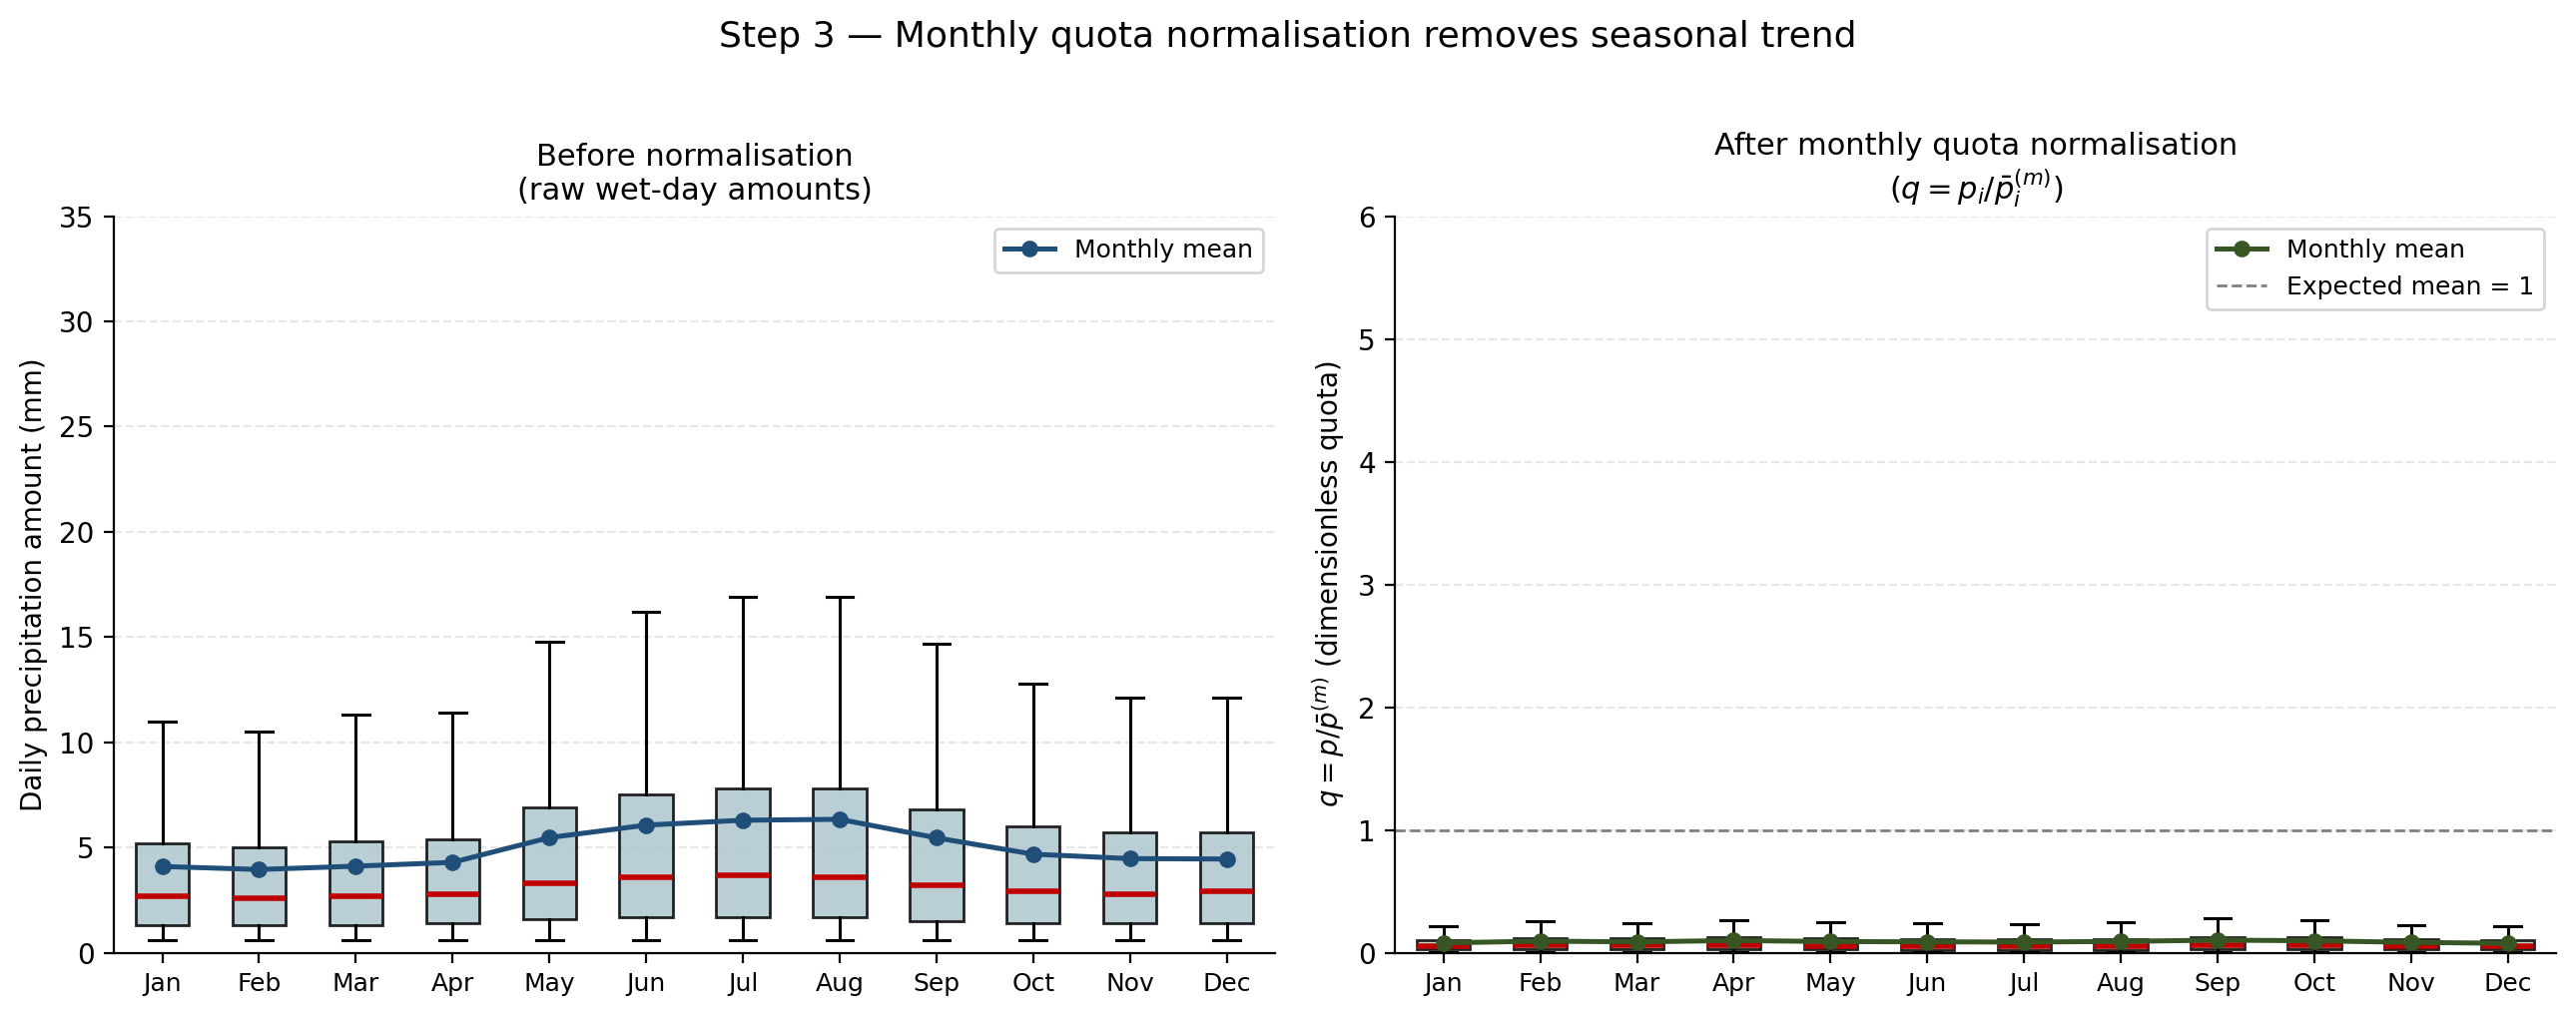
\includegraphics[width=0.95\textwidth]{images/04/prepro_seasonal}
    \caption{Monthly precipitation distributions before (left) and after
    (right) climatological normalisation. The seasonal cycle is removed
    and the distributions become approximately stationary across months}
    \label{fig:seasonal-normalisation}
\end{figure}

\subsection{Variogram fitting}
\label{sec:kriging-variogram}

Three variogram models (spherical, exponential, Gaussian) are fitted to the
pooled empirical semi-variance from all wet days of the full record
(1961--2023), following the climatological-variogram approach of
Section~\ref{sec:variogram_models} and the Marquardt weighted-least-squares
fit of Equation~\eqref{eq:marquardt-variogram}. Three transforms are tested
(none, log, normal-score), yielding nine fitted configurations in total.

\textbf{Discretisation parameters.}
The maximum lag is set to $h_{\max} = 416$~km (the 99th percentile of all
pairwise inter-station distances, Figure~\ref{fig:variogram-bins}), divided
into $N_{\text{lags}} = 38$ bins of width ${\approx}11$~km, fine enough to
resolve mesoscale structure while ensuring at least $N_{\min} = 30$ pairs per
bin \cite{cressie1993}. Under climatological pooling across all 63 years,
every bin contains several million pairs.

\begin{figure}[ht]
    \centering
    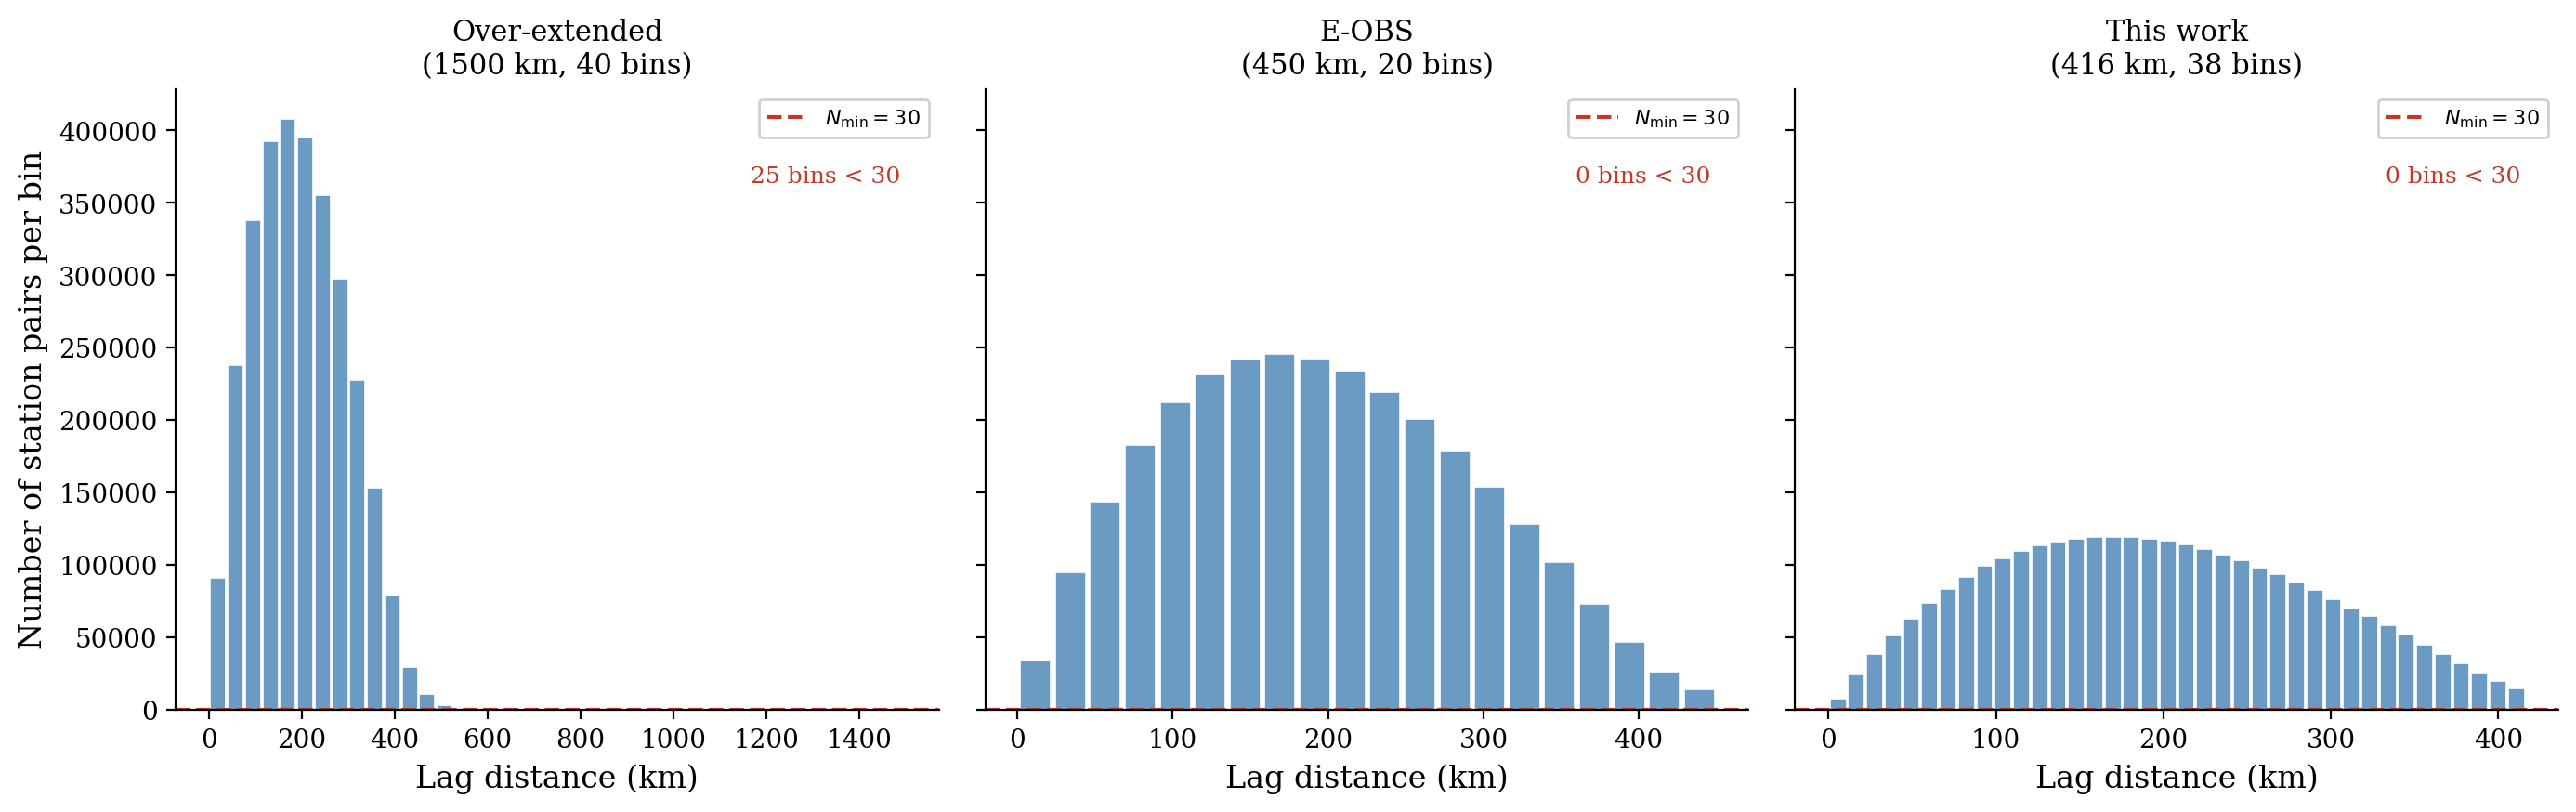
\includegraphics[width=0.95\textwidth]{images/04/variogram_bins}
    \caption{Variogram bin filling for three lag discretisations:
    over-extended (left), E-OBS settings (centre), and the settings adopted
    here (right, $h_{\max} = 416$~km, 38 bins). Red bars indicate bins with
    fewer than 30 pairs}
    \label{fig:variogram-bins}
\end{figure}

\begin{figure}[ht]
    \centering
    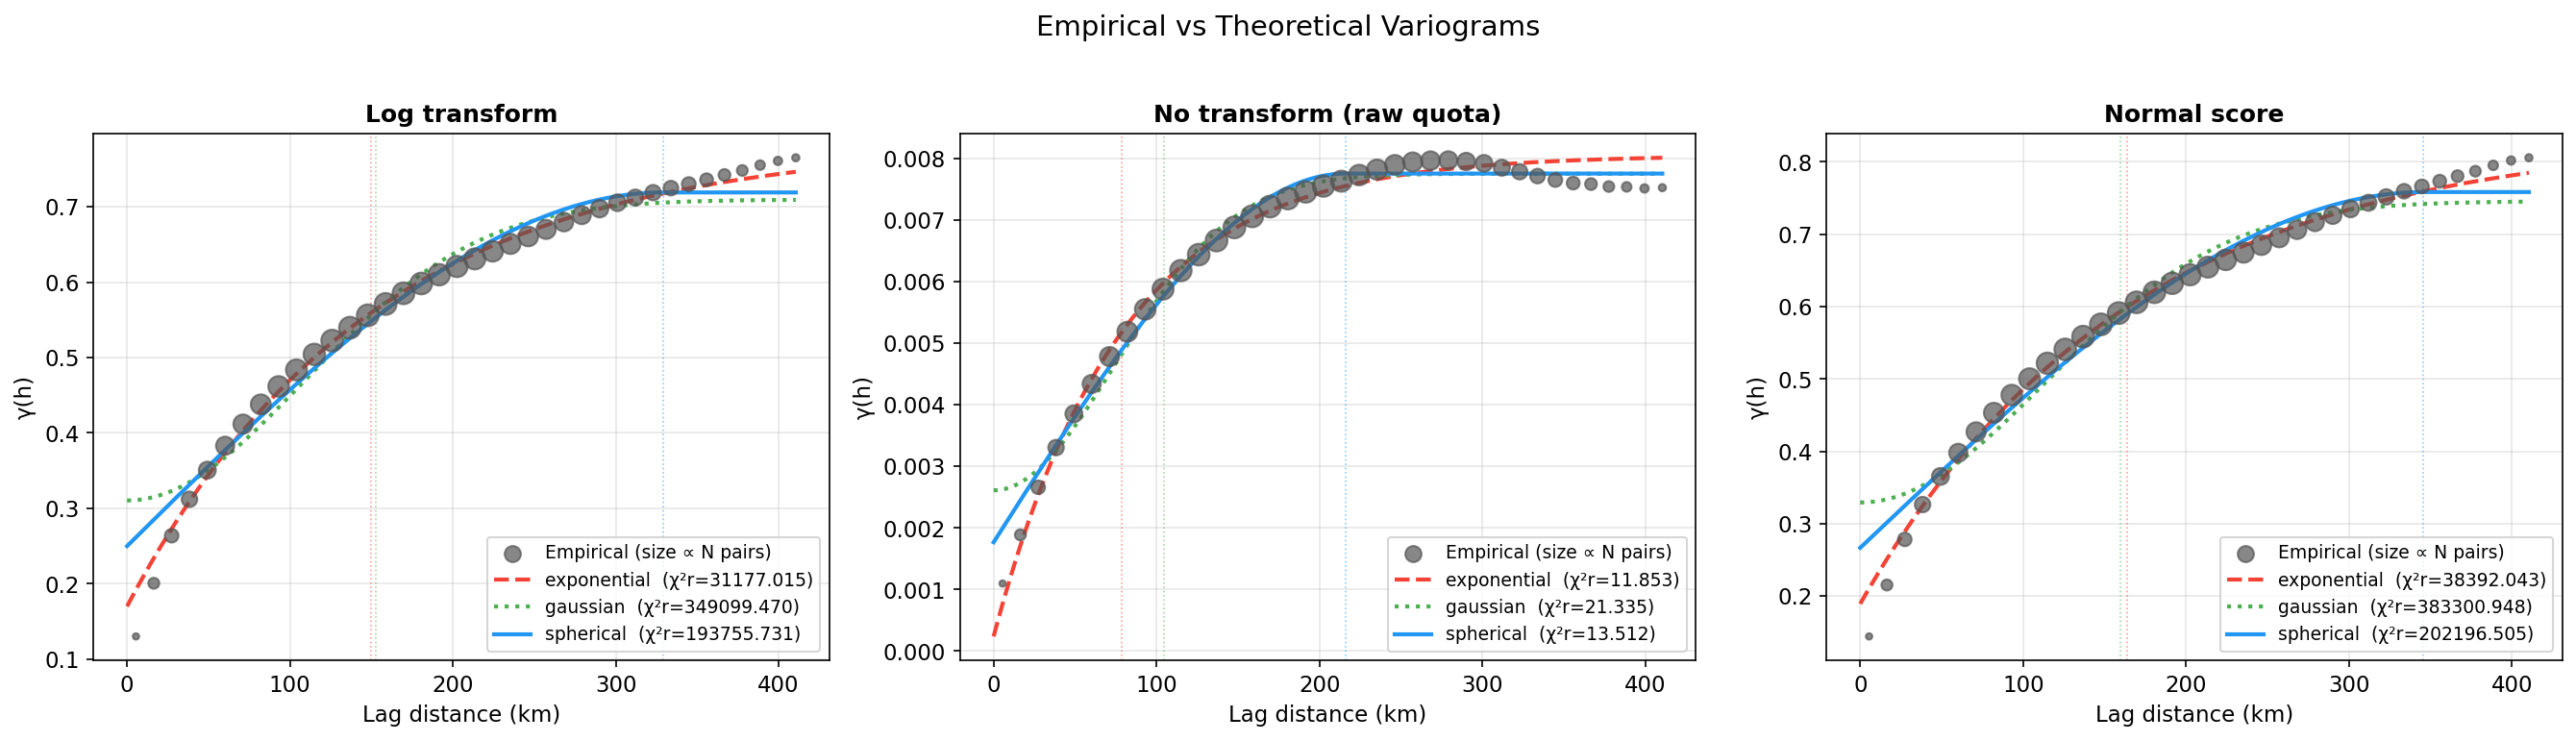
\includegraphics[width=0.95\textwidth]{images/04/variogram_fit}
    \caption{Empirical variograms with fitted models for log (left), raw
    ratio (centre), and normal-score (right) transforms. Point size is
    proportional to $N(h)$; $\chi^2_r$ is shown in the legend}
    \label{fig:variogram-fit}
\end{figure}

\begin{table}[ht]
    \centering
    \caption{Fitted variogram parameters for all nine
    (transform $\times$ model) configurations. Best $R^2$ within each
    transform is in bold.}
    \label{tab:variogram-params}
    \setlength{\tabcolsep}{4pt}
    \resizebox{\textwidth}{!}{%
    \begin{tabular}{ll ccccc}
    \toprule
    Transform & Model & Nugget $c_0$ & Sill $c_0{+}c_1$ & $a$ (km) & Eff.\ range (km) & $R^2$ \\
    \midrule
    \texttt{normal\_score} & spherical   & 0.267 & 0.754 & 342 & 342 & 0.965 \\
    \texttt{normal\_score} & exponential & 0.190 & 0.831 & 161 & 483 & \textbf{0.993} \\
    \texttt{normal\_score} & gaussian    & 0.329 & 0.742 & 158 & 273 & 0.933 \\
    \texttt{log}           & spherical   & 0.251 & 0.717 & 326 & 326 & 0.963 \\
    \texttt{log}           & exponential & 0.172 & 0.784 & 148 & 444 & \textbf{0.993} \\
    \texttt{log}           & gaussian    & 0.311 & 0.708 & 152 & 263 & 0.933 \\
    \texttt{none} (ratio)  & spherical   & 0.002 & 0.008 & 216 & 216 & 0.985 \\
    \texttt{none} (ratio)  & exponential & 0.000 & 0.008 &  79 & 236 & \textbf{0.986} \\
    \texttt{none} (ratio)  & gaussian    & 0.003 & 0.008 & 105 & 181 & 0.968 \\
    \bottomrule
    \end{tabular}%
    }
\end{table}

$R^2 = 1 - \mathrm{SS}_{\text{res}} / \mathrm{SS}_{\text{tot}}$ compares
the fitted variogram against the $N = 38$ empirical lag bins:
$\mathrm{SS}_{\text{res}}$ is the sum of squared residuals between
$\gamma_{\text{model}}(h_i)$ and $\hat{\gamma}(h_i)$, and
$\mathrm{SS}_{\text{tot}}$ is the variance of the empirical values
around their mean. Values close to $1$ indicate that the parametric
form tracks the empirical curve point-for-point; unlike $\chi^2_r$,
$R^2$ is scale-invariant and therefore directly comparable across
transforms operating in different z-spaces.

All nine configurations yield $R^2 \ge 0{.}93$, so the parametric
fits are sound and goodness-of-fit alone cannot rank them. The
selection between them is therefore decided by the cross-validated
CRPS in Section~\ref{sec:kriging-evaluation} rather than by the
variogram fit quality.

\subsection{Kriging prediction}
\label{sec:kriging-mechanics}

Given the fitted variogram, the ordinary kriging system of
Equation~\eqref{eq:kriging_system} is solved to obtain the optimal weights
$\mathbf{w}^*$ and the Lagrange multiplier $\lambda^*$, yielding the
kriging variance $\sigma^2_{\text{OK}}(\mathbf{s}_0)$ via
Equation~\eqref{eq:kriging_variance}. For brevity, $\sigma^2_K \equiv
\sigma^2_{\text{OK}}(\mathbf{s}_0)$ is used below.

A well-known property of $\sigma^2_K$ is that it depends only on station
geometry and the fitted variogram, not on the observed values
\cite{journel1989fundamentals, haylock2008european}. The Monte Carlo
back-transformation introduced below recovers intensity-dependent
uncertainty: the nonlinearity of $\varphi^{-1}$ stretches the same
$\sigma^2_K$ by different amounts depending on the rainfall intensity.

\subsubsection{Neighbourhood selection}
\label{sec:kriging-neighbourhood}

In practice, not every station participates in every grid-cell prediction.
The effective variogram range defines the distance beyond which spatial
correlation is negligible: for the spherical model it equals the range
parameter $a$ directly; for the exponential model it is $3a$ (the distance
at which $\gamma$ reaches 95\,\% of the sill); for the Gaussian model it
is approximately $\sqrt{3}\,a \approx 1.73a$.

For Stage~1 (indicator kriging), all stations within the domain participate
regardless of distance — the binary variable has a broader spatial
correlation than the precipitation amounts. For Stage~2 (amount kriging),
two restrictions are applied: only wet stations within the effective
range are considered, and when the number of wet stations exceeds a cap
of $k = 125$ only the $k$ nearest neighbours of each grid cell are kept.

\textbf{Screen effect.}
In a dense network, distant stations that lie ``behind'' closer ones
receive negative kriging weights: the information they carry is already
captured by the intervening stations, and they enter the kriging system
only as a minor trend-correction term \cite{deutsch1998gslib}. An empirical
analysis of the kriging weight distribution in this network shows that the
median number of stations carrying 90\,\% of the total positive weight is
approximately 26 (95th percentile: 34), and 99\,\% of the positive weight
is captured by a median of 51 stations. The cumulative weight curve
plateaus at 40--60 neighbours for the vast majority of days. Setting
$k = 125$ therefore preserves effectively all informative neighbours
while excluding the hundreds of distant stations that contribute only
noise through near-zero or negative weights.

\textbf{Sensitivity analysis.}
The value $k = 125$ is selected by cross-validation
(Figure~\ref{fig:sensitivity-max-wet}): CRPS is flat for $k \geq 50$, while
computation time grows steeply beyond that.

\begin{figure}[ht]
    \centering
    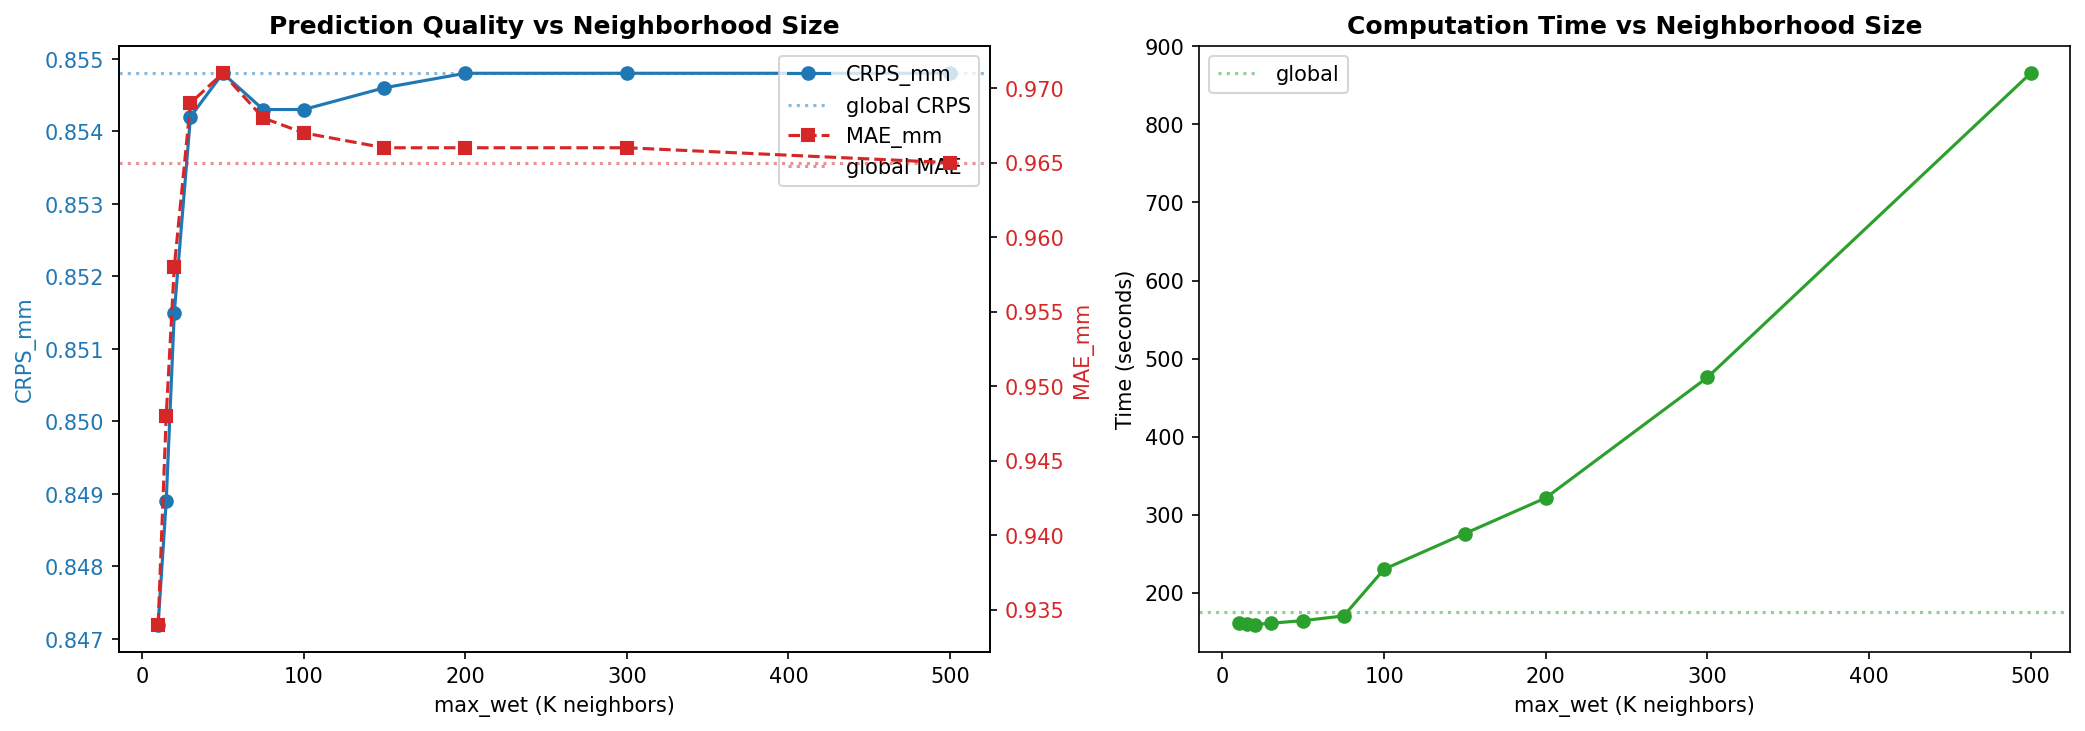
\includegraphics[width=0.95\textwidth]{images/04/sensitivity_max_wet}
    \caption{Cross-validated CRPS and computation time as a function of
    neighbourhood size $k$. Quality plateaus at $k \geq 50$; the selected
    value $k = 125$ is indicated}
    \label{fig:sensitivity-max-wet}
\end{figure}

No directional (octant or sector) search is applied. The spatial
correlation of precipitation in this domain is approximately isotropic
after climatological normalisation, so preferring stations from specific
compass directions offers no benefit over distance-based selection.

\subsubsection{Monte Carlo back-transformation}
\label{sec:kriging-mc}

The predicted ratio is obtained by drawing $K = 100$ samples from
$\mathcal{N}(\hat{z}_K, \sigma^2_K)$, back-transforming each via
$\varphi^{-1}$, and averaging \cite{journel1980lognormal}:
\begin{equation}
  \hat{Q}(\mathbf{s}_0) = \frac{1}{K}\sum_{k=1}^{K}
    \max\!\bigl(\varphi^{-1}(z^{(k)}),\, 0\bigr),
  \qquad
  \hat{Z}(\mathbf{s}_0) = \hat{Q}(\mathbf{s}_0) \times
    \bar{M}(\mathbf{s}_0, m).
  \label{eq:mc-backtrafo}
\end{equation}
The nonlinearity of $\varphi^{-1}$ produces intensity-dependent
uncertainty: variance is stretched more at high intensities than at low
ones.

%=============================================================================
\section{Cross-validation methodology}
\label{sec:kriging-cv-methodology}
%=============================================================================

For objective model selection, a \textbf{5-fold spatial cross-validation}
is used. The 2{,}458 stations are first split into 1{,}966 train and 492
holdout stations; the holdout set is never used for variogram fitting,
monthly-normal computation, or fold-internal training, and is reserved
for the cross-method evaluation of Chapter~\ref{ch:comparison}. The remaining
1{,}966 stations are partitioned into five folds via the canonical split
shared with the gradient boosting and BayesNF chapters
(\texttt{lgbm/fold\_assignment.parquet}), ensuring that all three models
are compared on identical fold assignments in Chapter~\ref{ch:comparison}.

For each fold $k$, the model is trained on the four other folds: monthly
TPS normals are refitted on the train-fold stations only, and predictions
are produced at the test-fold station coordinates. The global
climatological variogram from Section~\ref{sec:kriging-variogram} is
reused across all folds; an empirical check refits it independently on
each fold's train stations and confirms that the parameters drift by only
a few percent (variogram pooling dominates over the 20\,\% station
withdrawal because the pool aggregates ${\sim}10^{10}$ point pairs).

\textbf{Metrics.}
MAE (Equation~\eqref{eq:mae}) and CRPS (Section~\ref{sec:theory-crps}) are
the two metrics; CRPS is the primary one. For each held-out station the
$K = 100$ Monte Carlo back-transformed samples (Equation~\eqref{eq:mc-backtrafo})
form the predictive ensemble in millimetres, against which the fair CRPS
estimator (Equation~\eqref{eq:fair-crps}) is evaluated.
CRPS is computed in physical units rather than in $z$-space: different
transforms map identical physical errors to different magnitudes in
$z$-space, so evaluation in millimetres places all nine configurations
on equal footing.

%=============================================================================
\section{Cross-validation results and model selection}
\label{sec:kriging-evaluation}
%=============================================================================

Table~\ref{tab:kriging-cv} reports the cross-validation metrics for all
nine (transform $\times$ variogram) configurations, ranked by CRPS.
Metrics are computed on records on which the model predicts rainfall
($\hat{Z} \ge 0{.}4$~mm, $\approx 41\,\%$ of all records); this restricts
evaluation to the regime in which the amount stage is active.

\begin{table}[ht]
  \centering
  \caption{5-fold cross-validation results for Ordinary Kriging across all
  nine (transform $\times$ variogram) configurations (mean $\pm$ SD across
  folds). Best CRPS in bold.}
  \label{tab:kriging-cv}
  \begin{tabular}{ll cc}
    \toprule
    Transform & Variogram & MAE (mm) & CRPS (mm) \\
    \midrule
    \texttt{none} (ratio)  & exponential & $\mathbf{1.162 \pm 0.017}$ & $\mathbf{0.906 \pm 0.013}$ \\
    \texttt{normal\_score} & exponential & $1.194 \pm 0.017$ & $0.968 \pm 0.011$ \\
    \texttt{log}           & exponential & $1.203 \pm 0.017$ & $0.988 \pm 0.011$ \\
    \texttt{none} (ratio)  & spherical   & $1.347 \pm 0.017$ & $1.048 \pm 0.012$ \\
    \texttt{normal\_score} & spherical   & $1.306 \pm 0.017$ & $1.058 \pm 0.011$ \\
    \texttt{log}           & spherical   & $1.327 \pm 0.018$ & $1.093 \pm 0.011$ \\
    \texttt{normal\_score} & gaussian    & $1.579 \pm 0.016$ & $1.214 \pm 0.011$ \\
    \texttt{none} (ratio)  & gaussian    & $1.619 \pm 0.017$ & $1.219 \pm 0.012$ \\
    \texttt{log}           & gaussian    & $1.587 \pm 0.016$ & $1.245 \pm 0.011$ \\
    \bottomrule
  \end{tabular}
\end{table}

\begin{figure}[ht]
    \centering
    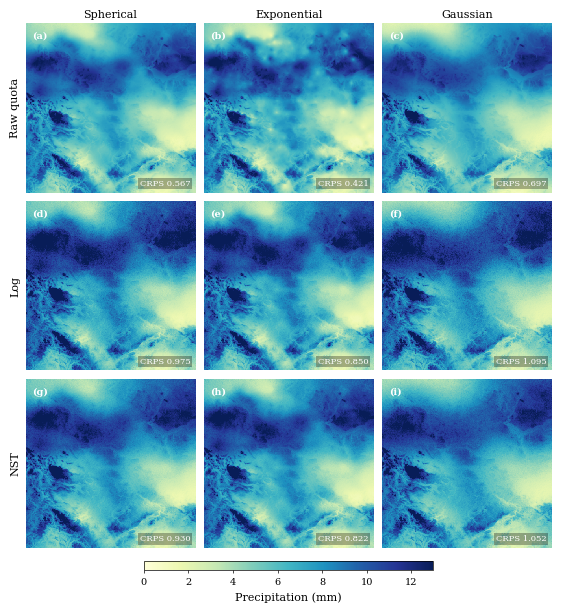
\includegraphics[width=0.95\textwidth]{images/04/predictions_all_combos}
    \caption{Spatial predictions for 1~February~2013 across all nine
    (transform $\times$ variogram) configurations}
    \label{fig:predictions-all-combos}
\end{figure}

\begin{figure}[ht]
    \centering
    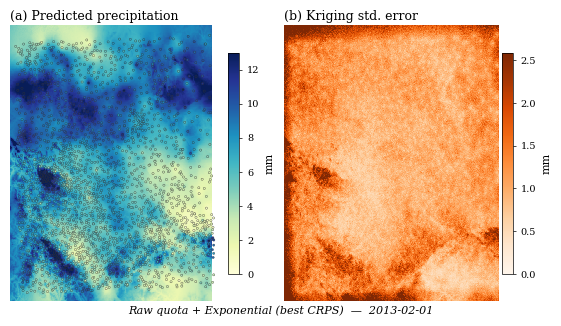
\includegraphics[width=0.95\textwidth]{images/04/best_pred_and_variance}
    \caption{Predicted precipitation (left) and kriging standard error
    (right) for the best-performing configuration (raw ratio $\times$
    exponential), 1~February~2013}
    \label{fig:best-pred-variance}
\end{figure}

\textbf{Variogram model choice.}
Haylock et al.~\cite[p.~5]{haylock2008european}, in the foundational
E-OBS methodology, tested five variogram models (Gaussian, exponential,
spherical, hole effect, power) for European precipitation kriging and
selected the model with the lowest $\chi^2$ statistic. For precipitation
amount, they found that \textit{``the modelled theoretical variograms are all
spherical, apart from precipitation amount which is exponential''}
\cite[p.~6]{haylock2008european}. The cross-validation results here
confirm this finding: for every transform, the exponential model
achieves the lowest CRPS, clearly outperforming the spherical and
Gaussian alternatives.

\textbf{Transform choice: why the raw ratio outperforms the Normal Score Transform.}
The Normal Score Transform has been recommended by Cecinati et
al.~\cite[p.~16]{cecinati2017} for kriging-based radar--gauge merging,
where it \textit{``achieves the best results overall''} among the tested
normalisation approaches. The cross-validation in this work, however,
finds that kriging on the raw climatological ratio (without any further
distributional transform) achieves a lower CRPS (0.906~mm) than the
normal-score variant (0.968~mm) or the log transform (0.988~mm).

Several factors explain this result. First, the climatological
normalisation (Section~\ref{sec:detrending}) already removes the
dominant source of non-stationarity: after detrending, the wet-day
ratios have a moderately right-skewed Gamma-like distribution, far from
the extreme skewness of raw precipitation. Second, the station network
is unusually dense (median nearest-neighbour distance of 2.1~km); in
dense networks, kriging weights are dominated by a few closest stations,
where spatial correlation is strong regardless of the distributional
shape. Third, the effective variogram range for the raw ratio
($3 \times 79 = 236$~km, exponential) is substantially shorter than for
the normal-score variant ($3 \times 161 = 483$~km), meaning the kriging
system operates with a compact, highly correlated neighbourhood instead
of mixing in weakly correlated distant stations.

Cecinati et al.~\cite{cecinati2017} evaluated the NST in the context of
Kriging with External Drift for radar--gauge merging, a setting with
additional covariates and sparser gauge networks, where enforcing
Gaussianity may provide a larger benefit. For Ordinary Kriging on
pre-detrended ratios with a dense station network, the simpler
approach without a transform suffices.

The configuration \texttt{none} $\times$ \texttt{exponential} is therefore
selected as the \textbf{final Ordinary Kriging implementation},
aligning the choice with Haylock et al.~\cite{haylock2008european} and
Hofstra et al.~\cite{hofstra2008comparison}, who use the same ratio
approach without a distributional transform for the E-OBS gridded
data set. It is the baseline against which gradient boosting
(Chapter~\ref{ch:gbm}) and Bayesian Neural Fields
(Chapter~\ref{ch:bayesnf}) are evaluated in
Chapter~\ref{ch:comparison}.

%=============================================================================
\section{Elevation contribution: 2D vs 3D TPS normals}
\label{sec:tps-experiment}
%=============================================================================

At holdout stations the station-specific monthly normal
$\bar{M}(\mathbf{s}_0, m)$ — required by the back-transformation
$\hat{Z} = \hat{Q}\,\bar{M}$
(Equation~\eqref{eq:back-transform}) — is unknown and must be interpolated
from the 1{,}966 train stations. Two TPS variants are compared: a 2D
surface fitted on projected coordinates $(x, y)$ and a 3D surface that
adds terrain elevation $(x, y, z_{\text{elev}})$. Both variants use the
same winning kriging configuration (raw ratio with the exponential
variogram) and the same 492 holdout stations; only the climatology
divisor changes.

Table~\ref{tab:tps-experiment} reports the cross-validated metrics on the
holdout set. The 3D variant reduces CRPS by 3.3\,\% and MAE by 4.2\,\%
relative to the 2D variant, confirming that elevation is an informative
covariate for the climatological field: in regions of
complex terrain, the orographic precipitation gradient cannot be captured
from planar coordinates alone, and the resulting normal estimates pass
this error through into the back-transformed amount. The 3D TPS variant
is therefore adopted as the operational climatology for the
cross-method evaluation of Chapter~\ref{ch:comparison}.

\begin{table}[ht]
  \centering
  \caption{2D vs 3D TPS monthly normals on the 492 holdout stations
  (winning combo: raw ratio $\times$ exponential), restricted to
  records on which the model predicts rainfall
  ($\hat{Z} \ge 0{.}4$~mm)}
  \label{tab:tps-experiment}
  \begin{tabular}{l cc}
    \toprule
    TPS mode & MAE (mm) & CRPS (mm) \\
    \midrule
    2D $(x, y)$              & 1.140 & 0.888 \\
    3D $(x, y, z_{\text{elev}})$ & \textbf{1.092} & \textbf{0.858} \\
    \midrule
    Relative improvement (3D over 2D) & $-4.2\%$ & $-3.3\%$ \\
    \bottomrule
  \end{tabular}
\end{table}


\chapter{Implementation of Gradient Boosting}
\label{ch:gbm}

%=============================================================================
\section{Pipeline overview}
\label{sec:lgbm-pipeline}
%=============================================================================

Gradient boosting is implemented as the first of the two machine-learning
baselines compared against Ordinary Kriging in
Chapter~\ref{ch:comparison}. The model is a direct probabilistic
regressor: the additive ensemble of Equation~\eqref{eq:gbm-additive} is
trained independently for a discrete grid of quantile levels using the
pinball loss of Equation~\eqref{eq:pinball}, so each station-day receives
an empirical predictive distribution rather than a single point
estimate. Three properties make LightGBM
\cite{ke2017lightgbm} a practical fit for this dataset: histogram-based
splitting (Section~\ref{sec:theory-lgbm}) handles the 17.4-million
wet-day records of the 1961--2023 archive without exhausting memory;
auxiliary covariates such as elevation and soil properties enter the
model directly, with no parametric stationarity assumption; and the
pinball objective is supported as a built-in loss, so the eleven
quantile boosters jointly form the predictive ensemble required for
CRPS evaluation (Section~\ref{sec:theory-crps}).

The same two-stage decomposition $Z = I \cdot A$ used by
Ordinary Kriging (Section~\ref{sec:kriging-indicator}) is preserved.
\emph{Stage~1} is a binary \texttt{LGBMClassifier} predicting the
wet-day indicator, which replaces indicator kriging and uses the
$\hat{p} > 0{.}4$ decision threshold of Hofstra et
al.~\cite{hofstra2008comparison}. \emph{Stage~2} is the eleven
quantile boosters trained on wet days only, which replace amount
kriging. The cells classified as dry by Stage~1 are clipped to zero
and bypass Stage~2. Figure~\ref{fig:lgbm-pipeline} illustrates the
full pipeline.

\begin{figure}[H]
    \centering
    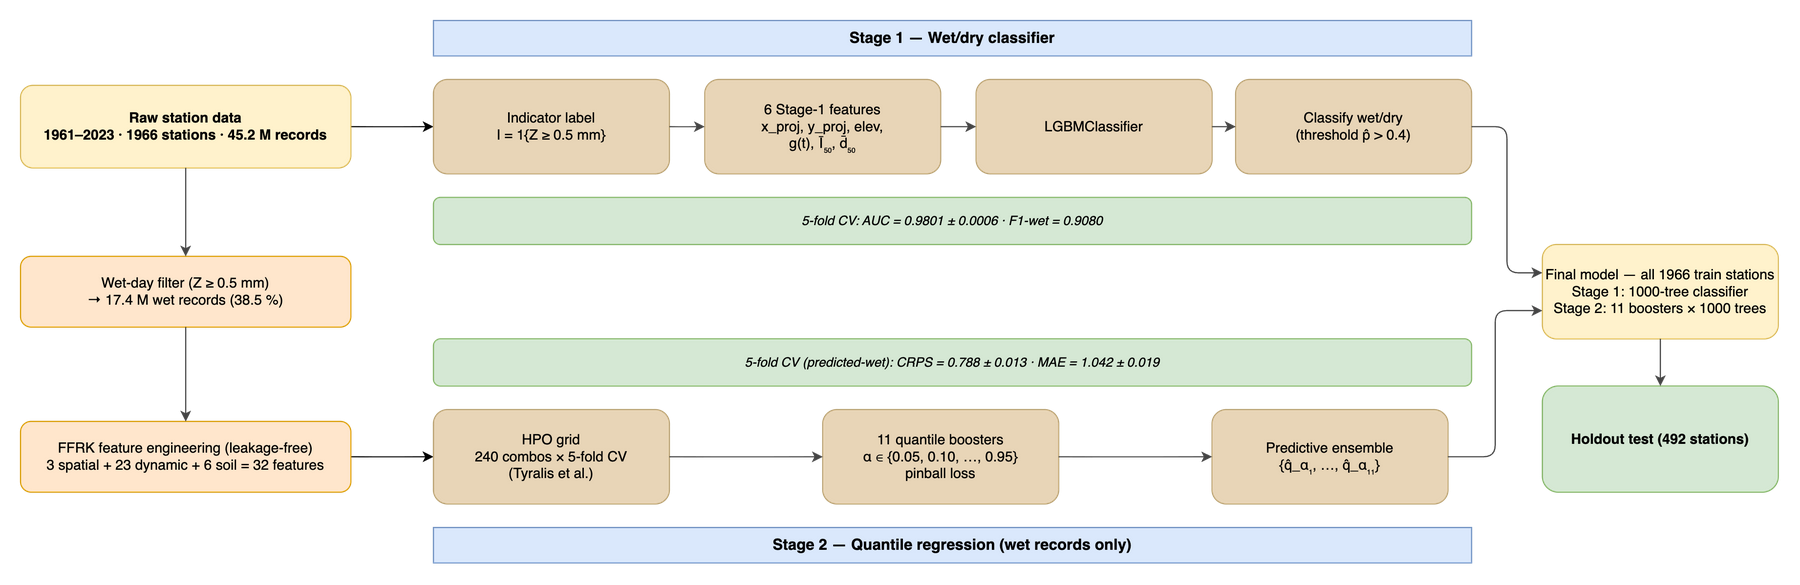
\includegraphics[width=\textwidth]{images/05/lgbm_pipeline}
    \caption{LightGBM two-stage pipeline. Stage~1 predicts the wet/dry
    indicator; Stage~2 trains eleven quantile boosters on wet records;
    HPO precedes Stage~2 training}
    \label{fig:lgbm-pipeline}
\end{figure}

%=============================================================================
\section{Stage~1: wet/dry classifier}
\label{sec:lgbm-stage1}
%=============================================================================

Stage~1 is a binary \texttt{LGBMClassifier} that predicts the wet-day
indicator $I(\mathbf{s}, t) = \mathbf{1}\{Z(\mathbf{s}, t) \ge
0{.}5\,\mathrm{mm}\}$ at every query location and date. Its feature
set is smaller than the 32-feature Stage~2 vector of
Section~\ref{sec:lgbm-features}: predicting whether it rained is a
binary decision dominated by the synoptic state and the local rainfall
area, whereas predicting \emph{how much} requires the full
distributional encoding of the neighbourhood. The six Stage~1 features
are listed in Table~\ref{tab:lgbm-stage1-features}.

\begin{table}[ht]
  \centering
  \caption{Input features for the LightGBM Stage~1 wet/dry classifier.
  The two kNN features pool the wet/dry indicator and the distance over
  the $K = 50$ nearest training neighbours of the query station; the
  global wet fraction is the per-day fraction of training stations with
  $Z \ge 0{.}5\,\mathrm{mm}$}
  \label{tab:lgbm-stage1-features}
  \begin{tabular}{l l l}
    \toprule
    Feature & Definition & Type \\
    \midrule
    $x_{\mathrm{proj}}$        & EPSG:3035 easting   & static  \\
    $y_{\mathrm{proj}}$        & EPSG:3035 northing  & static  \\
    \texttt{elevation\_m}      & Copernicus DEM-30   & static  \\
    \texttt{global\_wet\_frac} &
      $g(t) = \frac{1}{|\mathcal{S}_{\mathrm{tr}}|}
        \sum_{\mathbf{s} \in \mathcal{S}_{\mathrm{tr}}} I(\mathbf{s}, t)$
                                                    & per day \\
    \texttt{knn\_wet\_frac}    &
      $\bar{I}_K(\mathbf{s}, t) =
        \frac{1}{K} \sum_{j \in \mathcal{N}_K(\mathbf{s})} I(j, t)$
                                                    & per day \\
    \texttt{knn\_mean\_dist\_km} &
      $\bar{d}_K(\mathbf{s}) =
        \frac{1}{K} \sum_{j \in \mathcal{N}_K(\mathbf{s})}
          \|\mathbf{s} - j\|$                       & static  \\
    \bottomrule
  \end{tabular}
\end{table}

The features encode two complementary spatial scales of evidence. The
global wet fraction $g(t)$ summarises the synoptic state of day $t$: a
frontal passage produces high $g$ across the entire domain, while a
fair-weather day produces low $g$ everywhere. The kNN wet fraction
$\bar{I}_K(\mathbf{s}, t)$ summarises the local rainfall pattern in
the immediate neighbourhood of $\mathbf{s}$ on the same day,
distinguishing the wet sub-regions of an otherwise dry day (and vice
versa). The number of neighbours used in the kNN features is
$K = 50$, larger than the $K = 15$ used by Stage~2. The wet/dry
indicator carries less spatial noise than the amount field, so
averaging fifty indicators yields a stable rainfall-area estimate,
whereas averaging fifty amounts would blur the convective structure
that Stage~2 needs to resolve. As with the Stage~2 dynamic features,
the neighbour pool for $\bar{I}_K$ and the denominator of $g$ are
restricted to training stations only, so no leakage from holdout or
from the held-out fold during cross-validation can occur.

\paragraph{Hyperparameters.}
\begin{sloppypar}
The Stage~1 booster is fitted with the binary cross-entropy objective
and the settings $\texttt{n\_estimators} = 1000$,
$\texttt{learning\_rate} = 0{.}05$, $\texttt{num\_leaves} = 63$,
$\texttt{min\_child\_samples} = 50$, $\texttt{feature\_fraction} = 0{.}8$,
$\texttt{bagging\_fraction} = 0{.}8$ and $\texttt{bagging\_freq} = 1$.
Class imbalance is handled by setting
$\texttt{scale\_pos\_weight} = n_{\mathrm{dry}} / n_{\mathrm{wet}}$
computed on each fold's training set. Stage~1 hyperparameters were not
tuned on a grid: cross-validation AUC was already $0{.}98$ at the
defaults above, leaving little headroom for further tuning, so the
search budget was spent on the Stage~2 grid of
Section~\ref{sec:lgbm-training} instead.
\end{sloppypar}

\paragraph{Decision threshold.} At pipeline-inference time, a
station-day is forwarded to Stage~2 when
$\hat{p}_{\mathrm{wet}} > 0{.}40$, the same threshold used by the
indicator kriging step (Section~\ref{sec:kriging-indicator}, Hofstra
et al.~\cite{hofstra2008comparison}). Records below the threshold
receive a predictive distribution that is a point mass at zero,
equivalently an eleven-member ensemble of zeros at the Stage~2
quantile grid, so that the joint distribution feeding CRPS is
well-defined for every record. Lowering the threshold from the
conventional $0{.}50$ to $0{.}40$ trades a small increase in false
alarms for a substantial reduction in missed events, which is the
more expensive error class in CRPS terms: a missed wet day pays the
full observed amount, whereas a false alarm only pays the Stage~2
mean of the predicted ensemble.

\paragraph{Cross-validation performance.} Five-fold spatial
cross-validation on the canonical fold assignment of
Section~\ref{sec:lgbm-training} returns
ROC-AUC~$= 0{.}9801 \pm 0{.}0006$, Brier score
$= 0{.}0954 \pm 0{.}0009$, F1 on the wet class
$= 0{.}9080 \pm 0{.}0009$ and F1 on the dry class
$= 0{.}8908 \pm 0{.}0011$, all reported at the conventional
$\hat{p}_{\mathrm{wet}} > 0{.}50$ decision boundary. These scores
mirror the indicator-kriging skill of
Section~\ref{sec:kriging-indicator-impl}: the wet/dry binary is
highly separable at the 1~km daily aggregation, with the global wet
fraction $g(t)$ supplying the synoptic state and the kNN wet
fraction $\bar{I}_{50}(\mathbf{s}, t)$ resolving the local rainfall
area. The final classifier deployed in the combined pipeline is
trained on all $\sim$45.2 million station-days from the 1{,}966
training stations to 1{,}000 boosting rounds, with the kNN-derived
features recomputed once at full network density.

Figure~\ref{fig:lgbm-stage1-day} illustrates the Stage~1 wet/dry
mask on 15 July 2001, a summer convective day on which rainfall is
confined to the northern half of the domain. The classifier
reproduces the wet/dry boundary at the spatial resolution of the
1~km grid; residual misclassifications are concentrated along the
boundary itself, where the underlying probability
$\hat{p}_{\mathrm{wet}}$ transitions smoothly through the $0{.}40$
threshold.

\begin{figure}[ht]
    \centering
    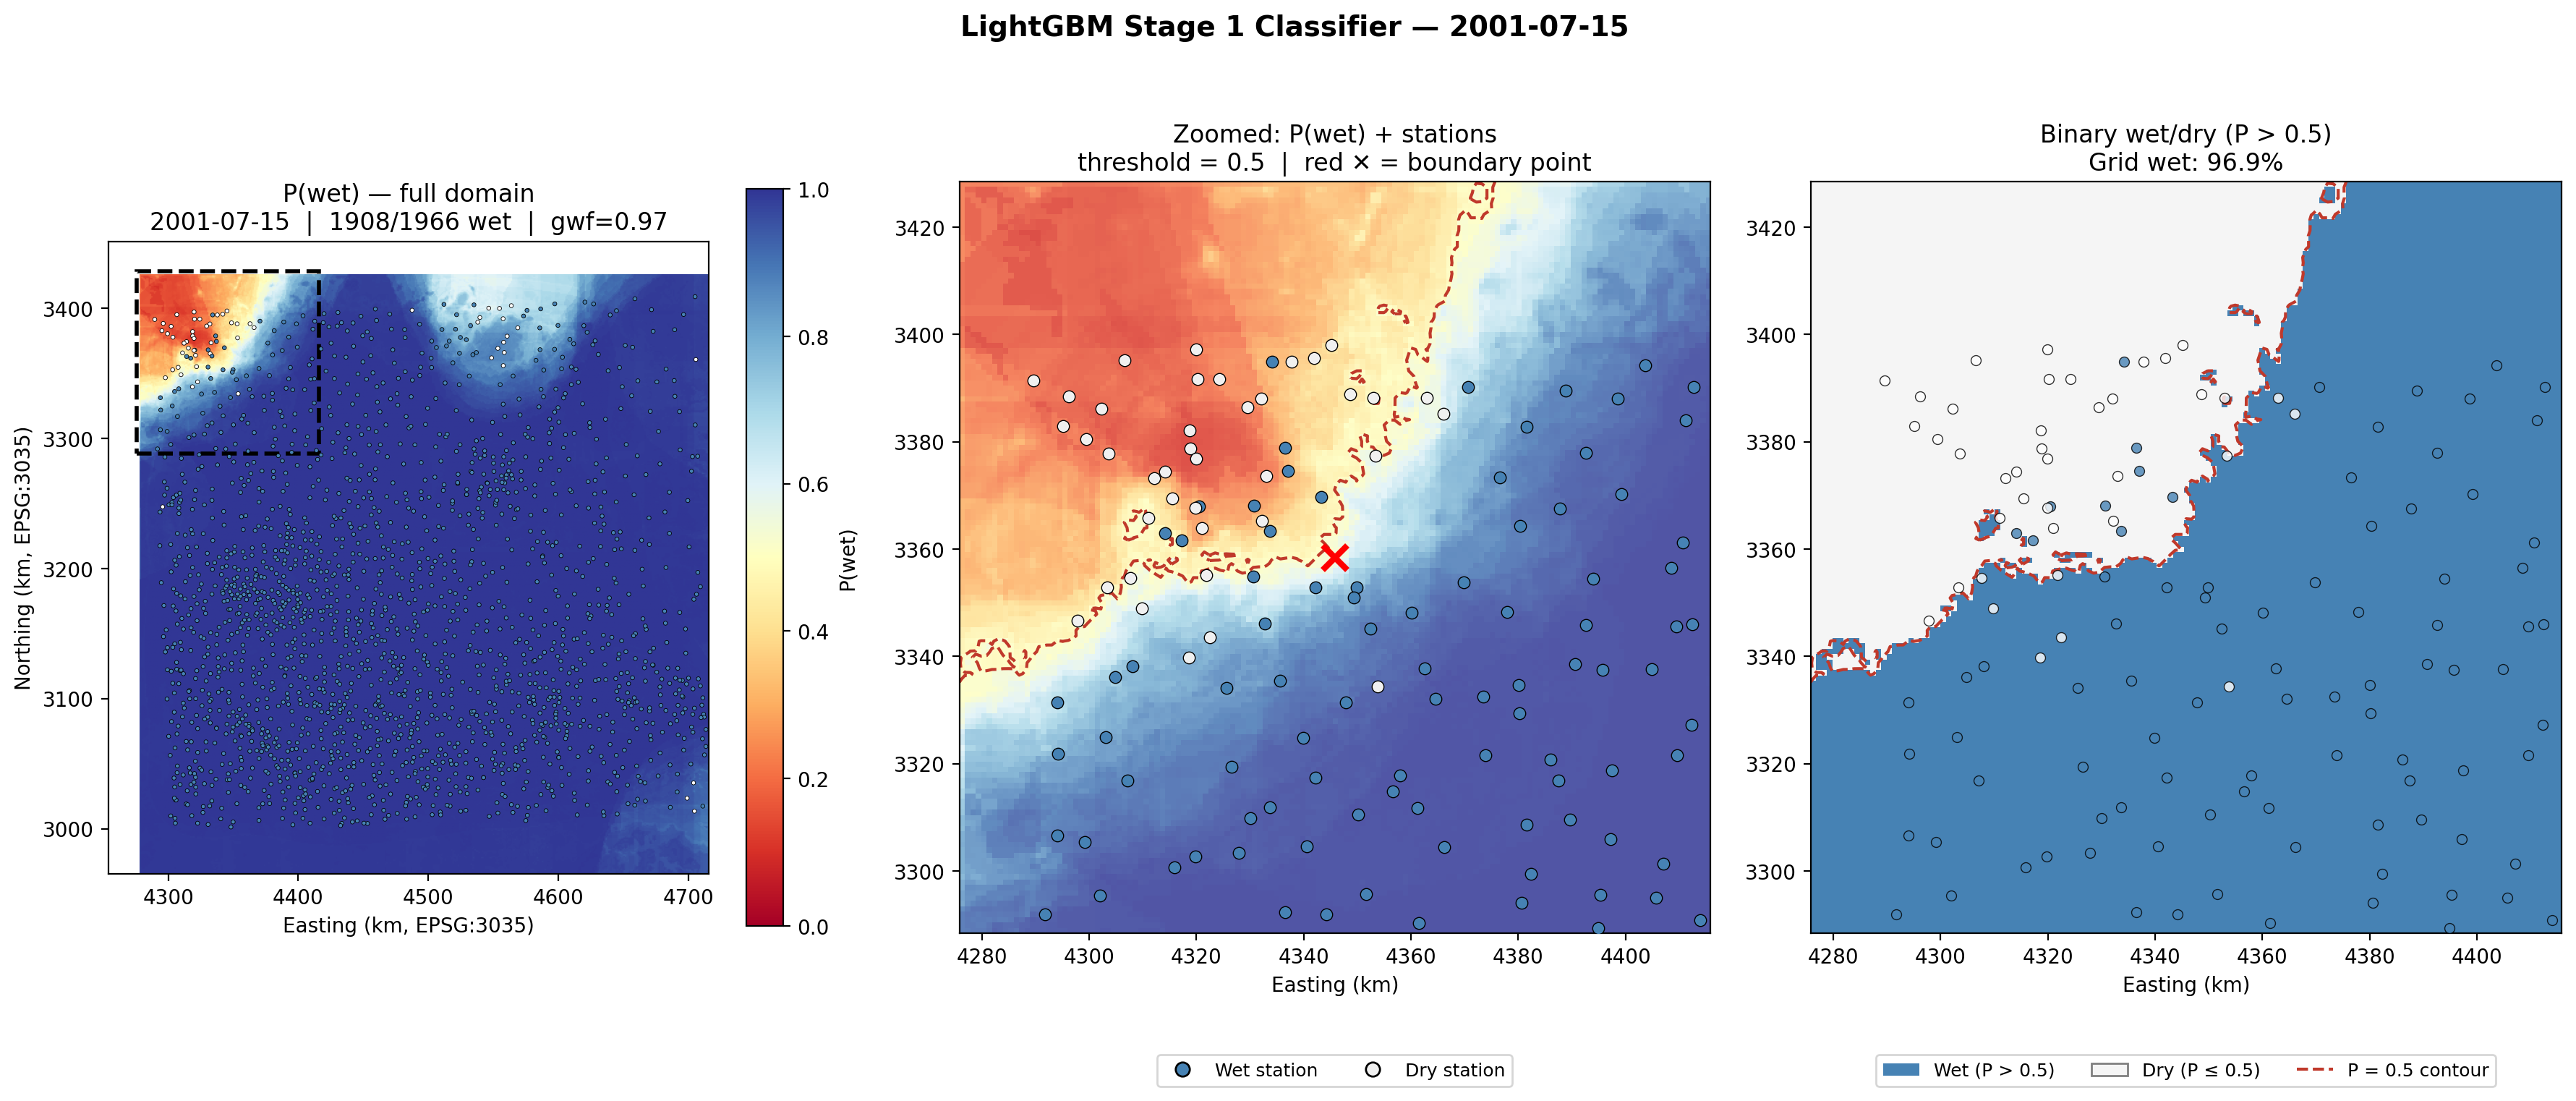
\includegraphics[width=0.95\textwidth]{images/05/lgbm_stage1_2001-07-15}
    \caption[Stage~1 wet/dry prediction for 15 July 2001]{Stage~1
    wet/dry prediction for 15 July 2001 on the 1~km EPSG:3035 grid.
    Left: predicted probability of rainfall $\hat{p}_{\mathrm{wet}}$.
    Right: binary wet/dry mask after applying the
    $\hat{p}_{\mathrm{wet}} > 0{.}40$ decision threshold. Station
    observations are overlaid as coloured discs}
    \label{fig:lgbm-stage1-day}
\end{figure}

%=============================================================================
\section{Stage~2: quantile regression}
\label{sec:lgbm-stage2}
%=============================================================================

\subsection{Why quantile regression}
\label{sec:lgbm-why-quantile}

Stage~2 predicts the rainfall amount conditional on a wet day. The
quantity of interest is not a single point estimate but the predictive
distribution $F_Z(z \mid \mathbf{s}, t)$, since CRPS
(Equation~\eqref{eq:crps}) and the calibration of prediction intervals
both require access to the full CDF. Quantile regression is the
natural fit for this requirement: a separate booster is trained for
each level $\alpha$ using the pinball loss
(Equation~\eqref{eq:pinball}), and the eleven predictions
$\{\hat{q}_{\alpha_1}, \ldots, \hat{q}_{\alpha_{11}}\}$ jointly form
an empirical predictive distribution that consumes the CRPS integrand
directly, with no parametric back-transformation. The two
alternatives explored before settling on direct quantile regression
were a regression-kriging hybrid (LightGBM trend plus Ordinary
Kriging on residuals) and parametric distribution-specific losses
(Tweedie, Gamma). The reasons for adopting direct quantile regression
are revisited in Section~\ref{sec:lgbm-discussion}.

\subsection{Feature engineering}
\label{sec:lgbm-features}

Gradient boosting requires that all spatial information be exposed as
explicit numerical features at the input layer. Whereas kriging
derives its spatial structure from the variogram, a tree ensemble has
no built-in notion of distance, isotropy or correlation: the network
geometry must be encoded manually. The feature engineering used here
follows the \emph{Feature-Free Regression Kriging} (FFRK) framework
of Luo, Wu and Song~\cite{luo2025featurefree}, in which three groups
of dynamic features (local dependence, local heterogeneity,
geosimilarity) capture the spatial structure that an external
covariate set would otherwise have to supply. To these dynamic
features, three projected spatial coordinates and six static
SoilGrids covariates are appended, yielding the 32-feature input
vector summarised in Table~\ref{tab:lgbm-features}.

\subsubsection*{Local dependence: inverse distance weighting}
\label{sec:lgbm-idw}

Local dependence is the tendency for nearby observations to take
similar values \cite{luo2025featurefree}. It is summarised at each
query location $\mathbf{s}_0$ by a single inverse-distance-weighted
average over its $K$ nearest wet-day neighbours
$\{\mathbf{s}_i\}_{i=1}^{K}$:
\begin{equation}
  f_{\mathrm{IDW}}(\mathbf{s}_0)
    = \frac{\sum_{i=1}^{K} w_i\, Z(\mathbf{s}_i)}{\sum_{i=1}^{K} w_i},
  \qquad
  w_i = \frac{1}{\|\mathbf{s}_0 - \mathbf{s}_i\|^{2} + \epsilon},
  \label{eq:lgbm-idw}
\end{equation}
with $K = 15$ and a numerical regulariser $\epsilon = 10^{-8}$~m$^2$
to prevent division by zero at coincident coordinates. The neighbour
count $K = 15$ is borrowed from the FFRK
paper~\cite{luo2025featurefree}, which adopts it from Song's GOS
work~\cite{song2022gos} and reports a sensitivity analysis confirming
the choice; the same value is therefore reused here without
re-tuning. The inverse-distance weighting produces a feature that
varies smoothly with the spatial density of nearby precipitation.
Because the same $K = 15$ neighbours are reused for the
heterogeneity and geosimilarity features below, the BallTree query
is performed once per day.

\subsubsection*{Local heterogeneity: SVD quantiles}
\label{sec:lgbm-svd}

A single weighted average compresses the neighbourhood into one
scalar and discards the shape of the local distribution. Local
heterogeneity is captured by encoding the empirical distribution of
the same $K$ neighbours as a vector of equally-spaced quantiles.
Following FFRK, twenty-one quantile levels
$\{0, 0{.}05, 0{.}10, \ldots, 0{.}95, 1\}$ are used:
\begin{equation}
  f_{\mathrm{SVD},q}(\mathbf{s}_0)
    = \mathrm{Quantile}_{q}\!\bigl(
        \{Z(\mathbf{s}_i)\}_{i=1}^{K}
      \bigr),
  \qquad q \in \{0, 0{.}05, \ldots, 1\},
  \label{eq:lgbm-svd}
\end{equation}
yielding twenty-one features \texttt{svd\_00}--\texttt{svd\_20}. The
full quantile profile encodes the minimum, median, maximum and
intermediate deciles of the local rainfall pattern in one shot,
exposing skewness and heavy-tail behaviour that an IDW average cannot
represent. The trees can then split on the upper-tail quantiles to
capture localised heavy events and on the lower-tail quantiles to
capture isolated dry patches inside a generally wet region.

\subsubsection*{Geosimilarity: GOS feature}
\label{sec:lgbm-gos}

Two query locations may share similar local rainfall
\emph{distributions} even when they are far apart, for instance two
stations in similar orographic settings on opposite sides of the
domain. The Geographically Optimal Similarity (GOS) framework of
Song~\cite{song2022gos} formalises this idea: the predictor at
$\mathbf{s}_0$ is a similarity-weighted mean of the values at
locations whose distributional profiles match that of $\mathbf{s}_0$.
Following FFRK, the profile vector at each neighbour is its own
SVD-quantile vector, the similarity is a Gaussian kernel of the
squared profile distance, and the GOS feature is the kernel-weighted
average:
\begin{equation}
  S_i =
    \exp\!\left(
      -\frac{
        \|\mathbf{p}_i - \mathbf{p}_0\|^{2}
      }{
        \sigma^{2}
      }
    \right),
  \qquad
  f_{\mathrm{GOS}}(\mathbf{s}_0)
    = \frac{\sum_{i=1}^{K} S_i\, Z(\mathbf{s}_i)}{\sum_{i=1}^{K} S_i},
  \label{eq:lgbm-gos}
\end{equation}
where $\mathbf{p}_0$ is the SVD-quantile vector at the query and
$\mathbf{p}_i$ at neighbour $i$, and $\sigma$ is a kernel bandwidth.
Compared with IDW, GOS down-weights neighbours whose distributional
shape diverges from the query's local pattern, even when they are
physically close, and up-weights neighbours that match the local
profile.

\subsubsection*{Static covariates}
\label{sec:lgbm-static}

The dynamic geo-features above describe the per-day point pattern but
encode no information about the underlying terrain or soil. Three
projected spatial coordinates and the six SoilGrids variables of
Section~\ref{sec:precip_statistics} are therefore appended as static
features: $x_{\mathrm{proj}}$ and $y_{\mathrm{proj}}$ in EPSG:3035
metres together with \texttt{elevation\_m} from the Copernicus DEM,
and the six SoilGrids predictors sampled at each station coordinate.

\subsubsection*{Feature inventory}
\label{sec:lgbm-feature-inventory}

Table~\ref{tab:lgbm-features} summarises the 32 input features that
enter each quantile booster. Three dynamic groups (IDW, SVD-quantiles,
GOS) are recomputed per day from the wet stations of that day; the
remaining nine features are station-level constants. The feature
importance ranking is reported in Section~\ref{sec:lgbm-discussion}.

\begin{table}[ht]
  \centering
  \caption{Input features for the LightGBM quantile boosters. The
  dynamic features (IDW, SVD, GOS) are recomputed each day from the
  $K = 15$ nearest wet-day neighbours; the static features are
  time-invariant per station}
  \label{tab:lgbm-features}
  \begin{tabular}{l c l l}
    \toprule
    Group              & Count & Source / formula
                                        & Type     \\
    \midrule
    Spatial            & 3     & EPSG:3035 + Copernicus DEM-30
                                        & static   \\
    IDW                & 1     & Equation~\eqref{eq:lgbm-idw}
                                        & per day  \\
    SVD-quantiles      & 21    & Equation~\eqref{eq:lgbm-svd}
                                        & per day  \\
    GOS                & 1     & Equation~\eqref{eq:lgbm-gos}
                                        & per day  \\
    SoilGrids          & 6     & SoilGrids 2.0 \cite{poggio2021soilgrids}
                                        & static   \\
    \midrule
    \textbf{Total}     & \textbf{32} &
                                        &          \\
    \bottomrule
  \end{tabular}
\end{table}

\subsection{Quantile grid and post-processing}
\label{sec:lgbm-quantiles}

The eleven quantile levels
\[
  \alpha \in
    \{0{.}05, 0{.}10, 0{.}20, 0{.}30, 0{.}40, 0{.}50,
      0{.}60, 0{.}70, 0{.}80, 0{.}90, 0{.}95\}
\]
are dense in the body of the distribution and span the central
90\,\% prediction interval at the extremes. One LightGBM booster is
trained independently for each $\alpha$ using the pinball loss of
Equation~\eqref{eq:pinball}; the ensemble of eleven predictions at
every station-day is the empirical predictive distribution that
feeds CRPS (Equation~\eqref{eq:crps}). Two cheap post-processing steps
are applied at inference time. First, each prediction is clipped to
be non-negative,
$\hat{q}_\alpha \leftarrow \max(\hat{q}_\alpha, 0)$, since
precipitation is non-negative. Second, the eleven predictions for a
given station-day are sorted in ascending order to repair occasional
quantile crossings introduced by the independent training of the
boosters. Both operations are deterministic and preserve the rank of
the predicted CDF.

\subsection{Training and hyperparameter tuning}
\label{sec:lgbm-training}

\paragraph{Data splitting.} The data partition follows
Section~\ref{sec:kriging-cv-methodology}: 1{,}966 train stations are
split into five folds via the canonical
\texttt{lgbm/fold\_assignment.parquet} file (${\sim}393$ stations
per fold), and the 492 holdout stations are reserved for the
cross-method evaluation of Chapter~\ref{ch:comparison}. The holdout
stations are excluded from hyperparameter optimisation, fold-level
training and feature recomputation, preventing leakage from train to
test through the dynamic geo-features.

\paragraph{Five-fold workflow.} Within each fold $k$, the four
other folds form the training set and the held-out fold is the test
set. Stage~1 is trained on every station-day record in the training
folds (wet and dry combined, $\sim$33~M records); Stage~2 is trained
only on the wet records ($\sim$13.9~M per fold). The dynamic
geo-features of Section~\ref{sec:lgbm-features} are recomputed for
every fold with the neighbour pool restricted to the four training
folds: a query station in the held-out fold $k$ retrieves its
$K = 15$ neighbours \emph{only from stations in folds $\ne k$}.
This prevents fold-internal information from leaking into the
test-fold features and is the LightGBM analogue of the fold-internal
variogram and monthly-normal refits used by Ordinary Kriging
(Section~\ref{sec:kriging-cv-methodology}).

\paragraph{Hyperparameter grid.}
\begin{sloppypar}
The four most influential LightGBM hyperparameters are tuned on a grid
inspired by Tyralis et al.~\cite{tyralis2023lightgbm}:
\texttt{max\_depth} $\in \{6, 8, 10\}$, \texttt{num\_leaves}
$\in \{20, 40, 60, 80, 100, 200, 500\}$ filtered to satisfy
$\texttt{num\_leaves} \le 2^{\texttt{max\_depth}}$,
\texttt{learning\_rate} $\in \{0{.}02, 0{.}05, 0{.}1\}$, and
\texttt{min\_child\_samples} $\in \{20, 100, 200, 500, 1000\}$.
After filtering, 240 valid combinations remain. Each combination is
evaluated by the mean CRPS across the five spatial folds defined
above. Per combination, the full quantile grid of
Section~\ref{sec:lgbm-quantiles} is trained on each fold, for a
total of $240 \times 11 \times 5 = 13{,}200$ boosters in the search.
\end{sloppypar}

\subsection{HPO results}
\label{sec:lgbm-hpo}

Figure~\ref{fig:lgbm-hpo} summarises the 240-combination grid
search. The left panel shows the marginal mean cross-validated CRPS
for each (\texttt{max\_depth}, \texttt{learning\_rate}) pair
averaged over leaves and minimum-child constraints; the three right
panels show the marginal distribution of cross-validated CRPS along
each remaining axis, with the within-axis minimum marked separately
from the within-axis mean. Cross-validated CRPS spans a narrow range
of $0{.}5195$--$0{.}5321$ across the grid (median $0{.}5231$,
standard deviation $0{.}003$), indicating that LightGBM is stable to
the choice of these four hyperparameters in the regime explored. This
narrow spread is partly attributable to the strong predictive signal of
the FFRK-derived geofeatures (Section~\ref{sec:lgbm-features}): IDW,
the SVD quantile profile and GOS already account for much of the
spatial and distributional structure, so the residual modelling task
faced by LightGBM is robust to hyperparameter perturbations within the
explored range. The
optimum lies at \texttt{max\_depth}~$= 10$,
\texttt{num\_leaves}~$= 200$, \texttt{learning\_rate}~$= 0{.}05$,
\texttt{min\_child\_samples}~$= 100$ with cross-validated mean
CRPS~$= 0.5195$~mm. Leaf-wise growth with a large leaf budget
benefits from the 13.9-million-record training pool, and the
$\texttt{min\_child\_samples}~= 100$ choice is a moderate
regularisation that prevents over-fitting on the dense central body
of the distribution while still letting the tail quantiles split.
This combination is fixed for the per-fold reporting of
Section~\ref{sec:lgbm-cv-results} and for the final all-data model
used in Chapter~\ref{ch:comparison}.

\begin{figure}[ht]
    \centering
    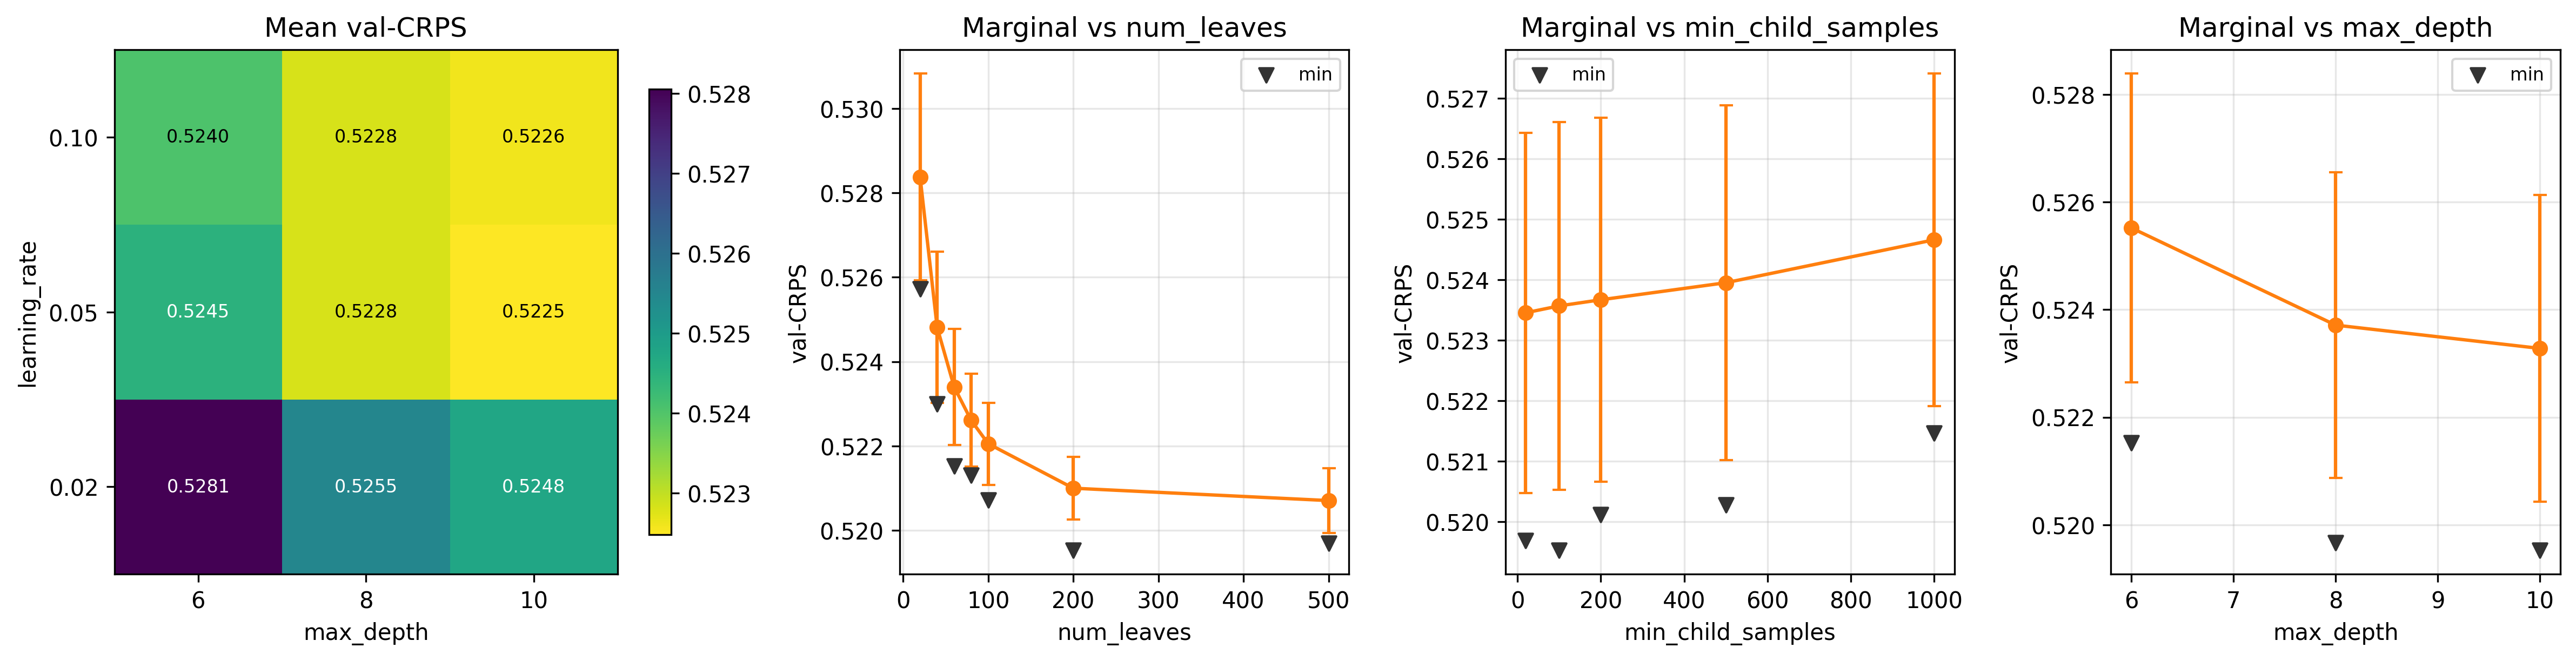
\includegraphics[width=0.99\textwidth]{images/05/lgbm_hpo}
    \caption{Hyperparameter optimisation over the 240-combination
    grid. Left: mean fold-averaged CRPS as a function of
    \texttt{max\_depth} and \texttt{learning\_rate}. Right: marginal
    fold-averaged CRPS along the \texttt{num\_leaves},
    \texttt{min\_child\_samples} and \texttt{max\_depth} axes; the
    orange curves show the per-axis mean with $\pm 1\sigma$ error
    bars and the black markers indicate the per-axis minimum}
    \label{fig:lgbm-hpo}
\end{figure}

\clearpage

%=============================================================================
\section{Cross-validation results}
\label{sec:lgbm-cv-results}
%=============================================================================

\subsection{Per-fold CRPS and MAE}
\label{sec:lgbm-perfold}

Table~\ref{tab:lgbm-cv} reports the per-fold CRPS and MAE for the
five-fold cross-validation. The standard deviation across folds is
small (${\approx}1{.}6\,\%$ of the mean for CRPS) and consistent
with the homogeneous spatial coverage of the fold partition.

\begin{table}[ht]
  \centering
  \caption{5-fold cross-validation results for LightGBM. Each row
  reports the CRPS and MAE on the held-out fold, computed in
  physical millimetres on the predicted-wet records. The last row
  reports the mean across folds with the corresponding standard
  deviation}
  \label{tab:lgbm-cv}
  \begin{tabular}{c r r r}
    \toprule
    Fold & $n_{\mathrm{test}}$ & MAE (mm) & CRPS (mm) \\
    \midrule
    0 & 3{,}520{,}827 & 1.066 & 0.804 \\
    1 & 3{,}466{,}145 & 1.056 & 0.796 \\
    2 & 3{,}495{,}450 & 1.040 & 0.787 \\
    3 & 3{,}471{,}152 & 1.023 & 0.774 \\
    4 & 3{,}452{,}880 & 1.024 & 0.777 \\
    \midrule
    \textbf{Mean} & --- & $\mathbf{1.042 \pm 0.019}$
                       & $\mathbf{0.788 \pm 0.013}$ \\
    \bottomrule
  \end{tabular}
\end{table}


\subsection{Error stratification}
\label{sec:lgbm-errors}

Figure~\ref{fig:lgbm-crps-intensity} stratifies the OOF CRPS by
true precipitation intensity. Light to moderate rainfall events
(0.5--10~mm) dominate the record and are predicted with
sub-millimetre CRPS. Skill degrades approximately linearly on the
upper tail: the heaviest bin ($\geq 50$~mm) reaches CRPS values an
order of magnitude larger than the body.
Figure~\ref{fig:lgbm-spatial-errors} maps the per-station OOF MAE
across the study area; errors are spatially smooth and concentrated
along the elevated south-eastern corner of the domain, mirroring
the pattern observed in the kriging cross-validation
(Section~\ref{sec:kriging-evaluation}).

\begin{figure}[H]
    \centering
    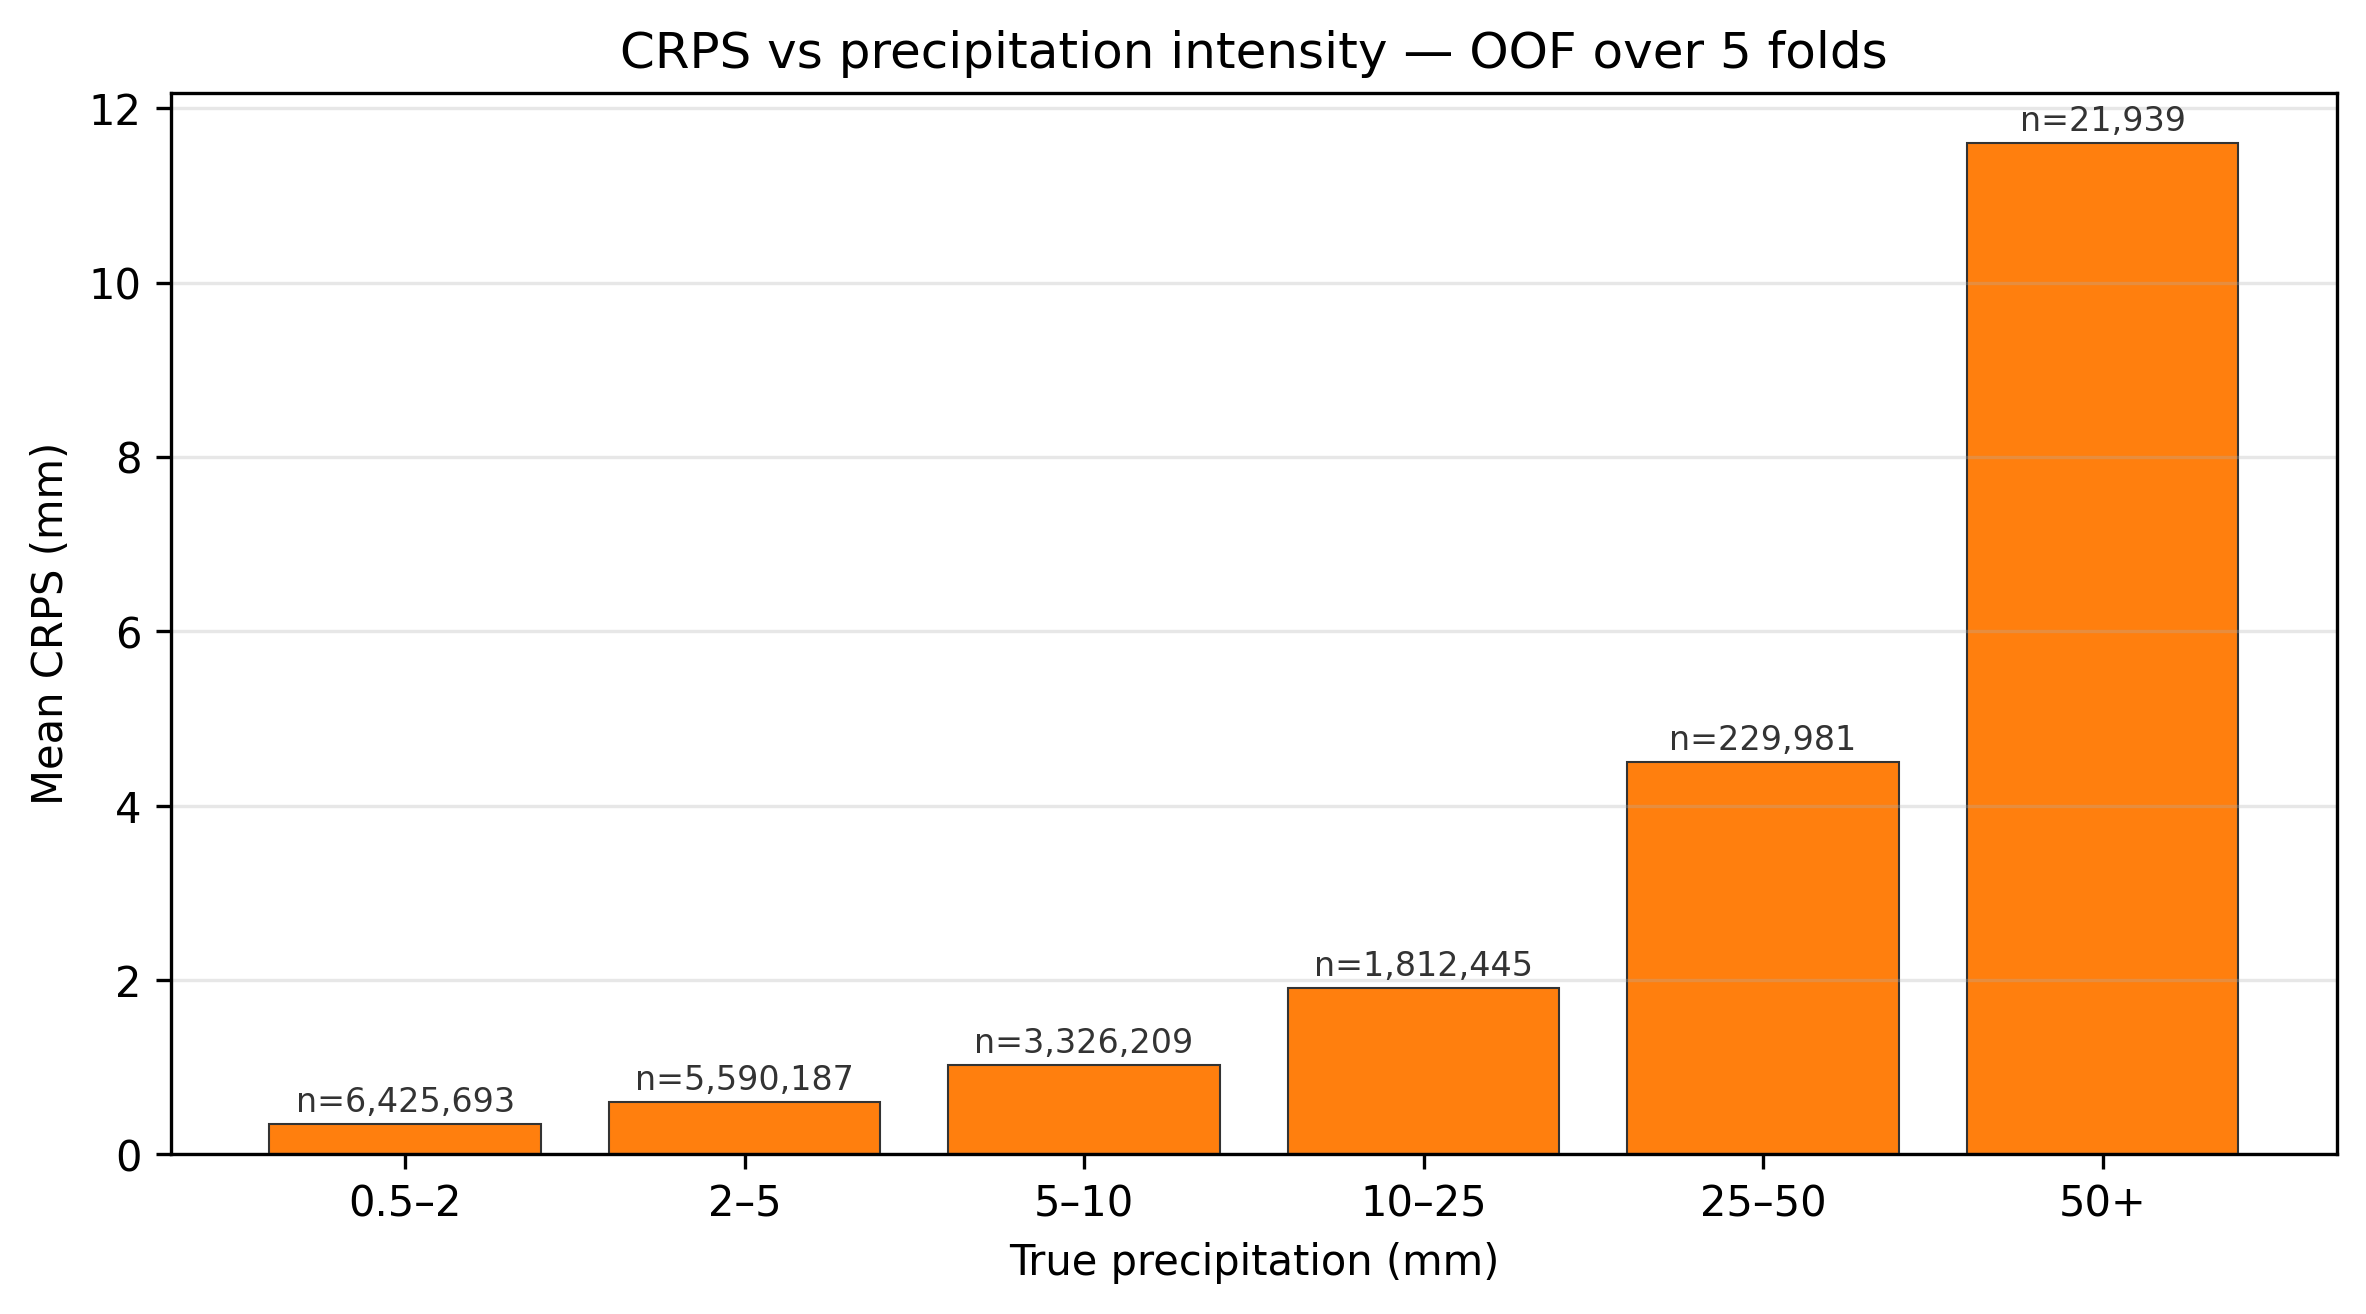
\includegraphics[width=0.85\textwidth]{images/05/lgbm_crps_by_intensity}
    \caption{Out-of-fold CRPS stratified by true precipitation
    intensity. Bars annotated with the bin sample size $n$}
    \label{fig:lgbm-crps-intensity}
\end{figure}

\begin{figure}[H]
    \centering
    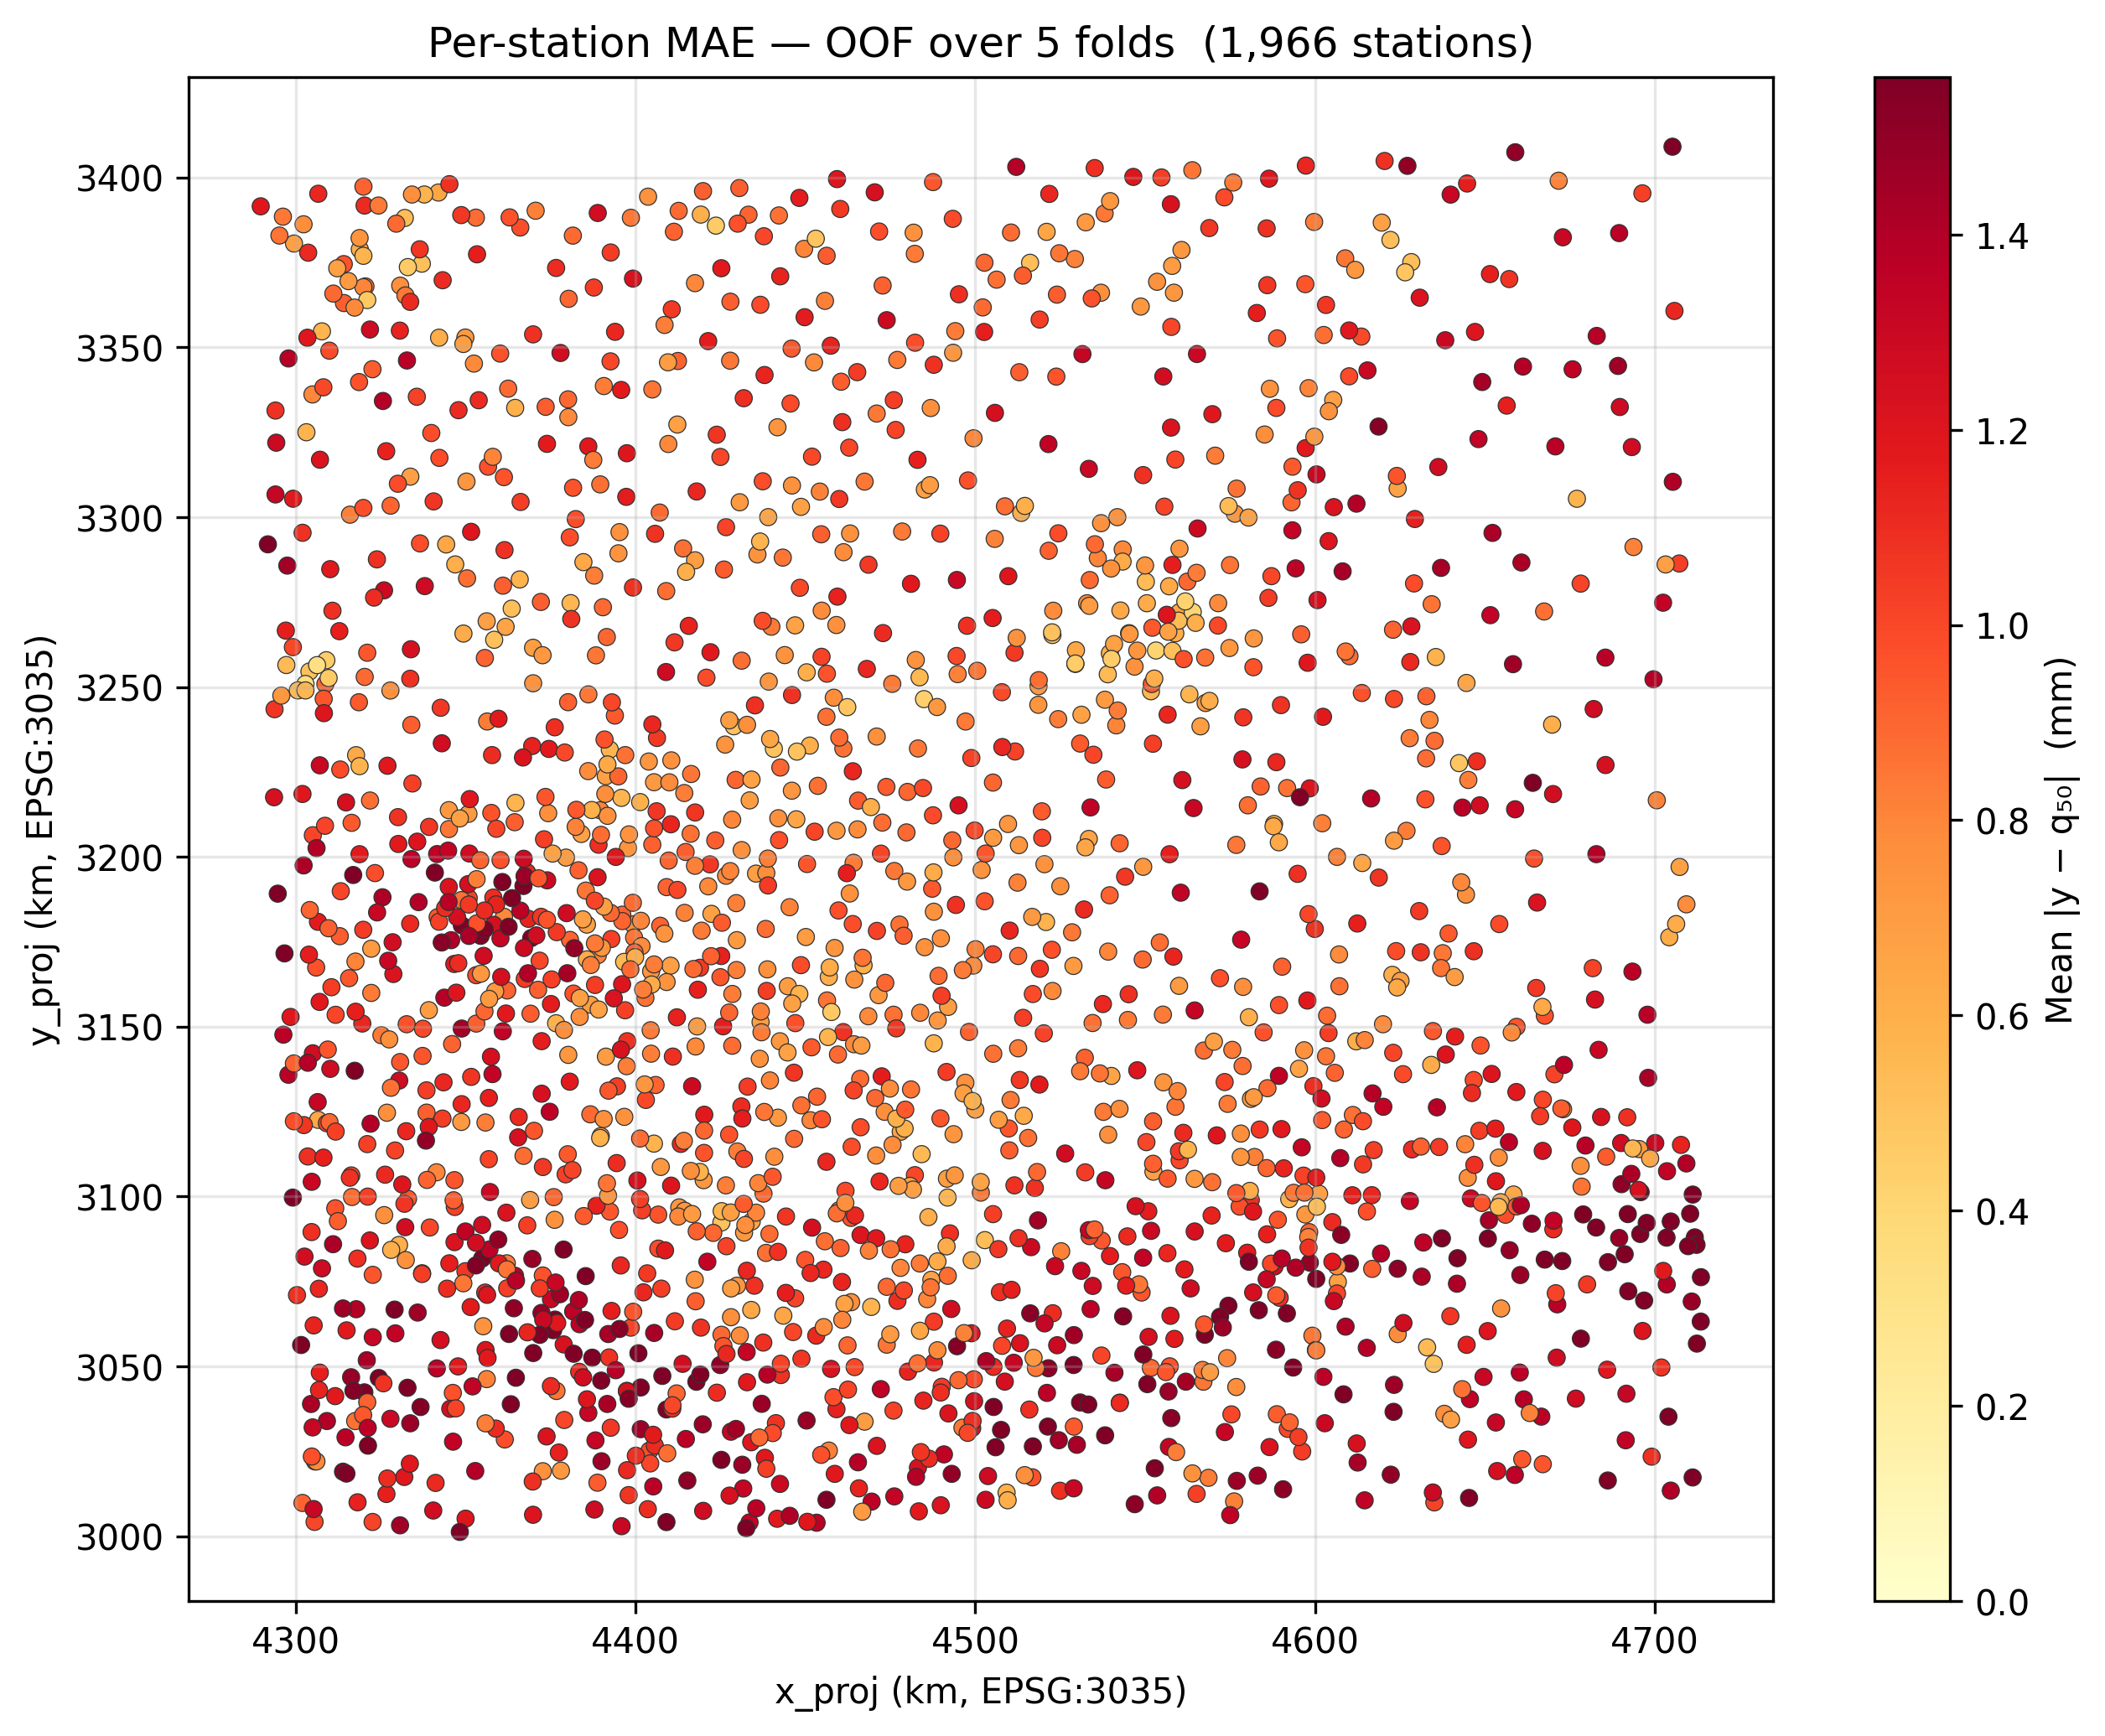
\includegraphics[width=0.85\textwidth]{images/05/lgbm_spatial_errors}
    \caption{Per-station out-of-fold MAE across the study area.
    Each station appears in exactly one fold's test side, so the
    colour at a point is the OOF mean residual at that location}
    \label{fig:lgbm-spatial-errors}
\end{figure}
\clearpage

%=============================================================================
\section{Discussion}
\label{sec:lgbm-discussion}
%=============================================================================

\subsection{Feature importance}
\label{sec:lgbm-feature-importance}

\begin{figure}[H]
    \centering
    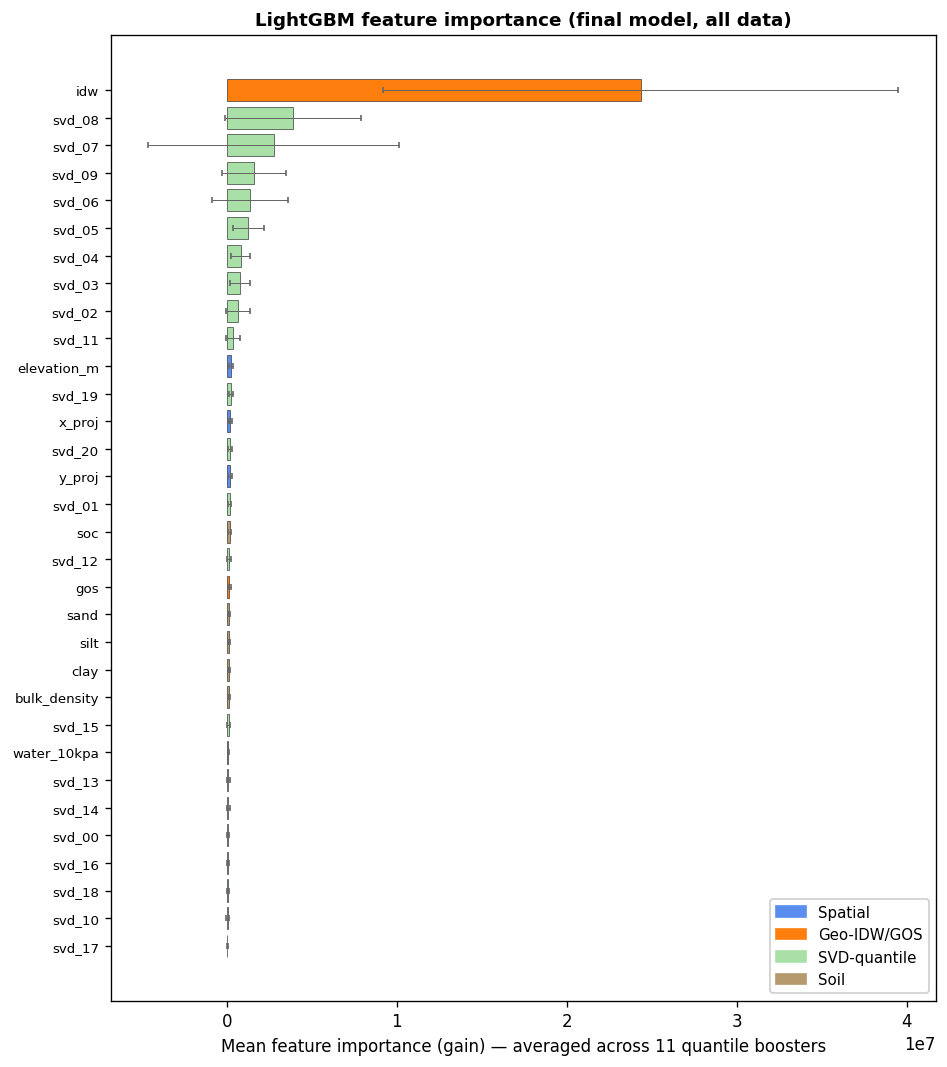
\includegraphics[width=0.48\textwidth]{images/05/features_importants_gain}\hfill
    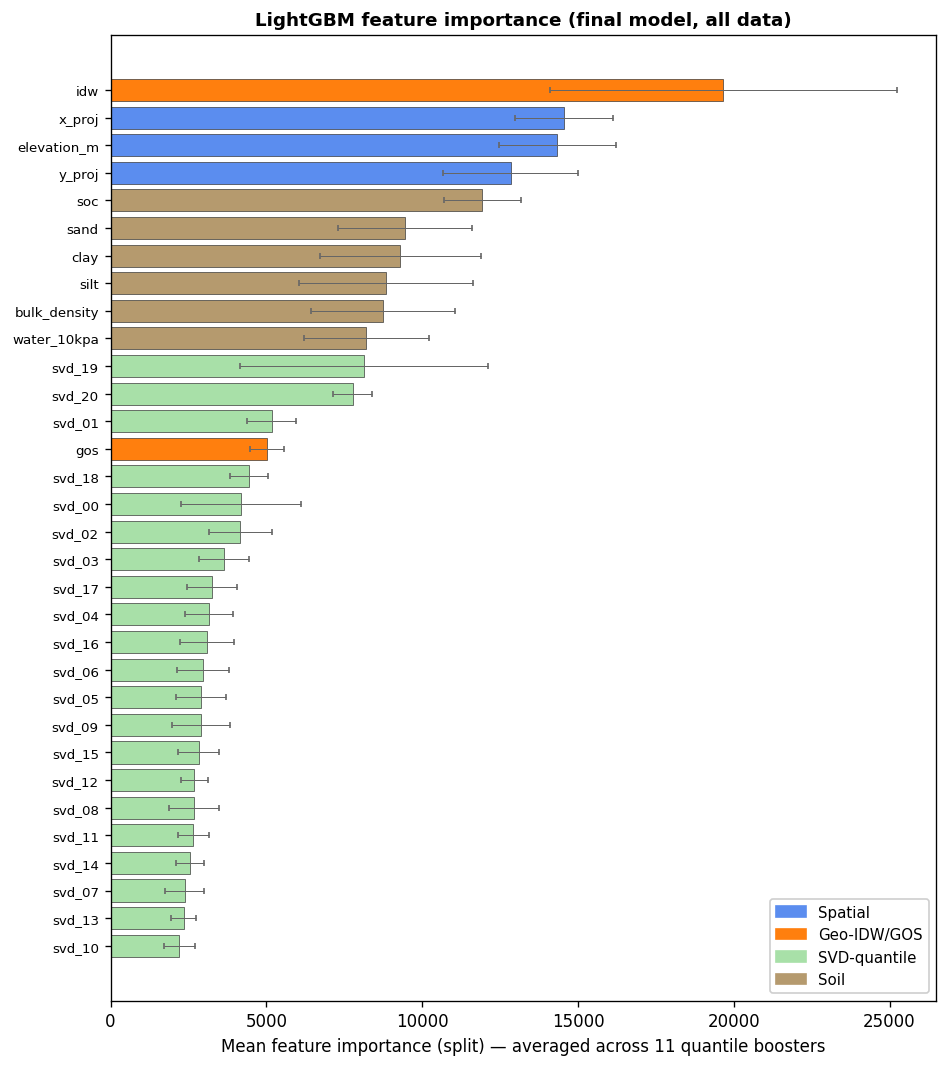
\includegraphics[width=0.48\textwidth]{images/05/features_importants_split}
    \caption{LightGBM feature importance averaged across the eleven
    quantile boosters of the final model, ranked by two complementary
    metrics. Left: \emph{gain} importance, the total reduction in
    pinball loss attributed to each feature across all splits. Right:
    \emph{split count}, the number of times each feature is used as a
    split variable. Bars are colour-coded by feature group; error bars
    indicate the cross-quantile standard deviation}
    \label{fig:lgbm-features}
\end{figure}

Figure~\ref{fig:lgbm-features} reports the per-feature importance under
both LightGBM metrics. The two views tell complementary stories.

By \emph{gain}, the inverse-distance-weighted mean \texttt{idw} dominates
by a wide margin, followed by a second tier of central SVD-quantiles
(\texttt{svd\_07}--\texttt{svd\_09}). A single split on \texttt{idw}
captures most of the spatial signal in the target, because the average of
the $K=15$ nearest wet-day neighbours is by itself a strong predictor of
the local precipitation amount. The central SVD-quantiles refine that
prediction on heterogeneous neighbourhoods where the mean alone
under-describes the rainfall pattern.

By \emph{split count}, the static spatial coordinates
($x_{\mathrm{proj}}$, $y_{\mathrm{proj}}$, \texttt{elevation\_m}) and the
SoilGrids covariates contribute substantially: each receives many splits
even though every individual split contributes little to the loss
reduction. This is the typical signature of \emph{local fine-tuning
features}: once the dominant \texttt{idw}/SVD signal has been captured by
a few high-gain splits, the trees use the static covariates repeatedly to
correct the residuals in narrow regions of the feature space. The two
metrics therefore agree on the hierarchy of the dynamic FFRK features as
the principal signal carriers, while showing that the static spatial and
soil covariates are not redundant: they are used frequently, but for a
different purpose.

\subsection{Why no residual kriging}
\label{sec:lgbm-rk-ablation}

The choice of direct quantile regression over a regression-kriging
hybrid (LightGBM trend plus Ordinary Kriging on residuals) was
guided by a dedicated ablation on the same 5-fold partition used for
the main model (Section~\ref{sec:lgbm-training}). The dynamic
neighbourhood feature set (IDW, SVD-quantiles, geographically
oriented statistics) already absorbs the spatial signal, so the
residual field is near-white-noise spatially: the fitted residual
variogram exhibits a pure-nugget structure with negligible
psill-to-sill ratio. Kriging an essentially uncorrelated residual
field adds variance without reducing bias, and the hybrid model
underperformed direct quantile regression on holdout CRPS in every
fold. Direct quantile regression is therefore preferred: fewer
moving parts and a closed-form CRPS via the eleven-member ensemble,
with no parametric back-transformation step.

\chapter{Implementation of Bayesian Neural Fields}
\label{ch:bayesnf}

This chapter documents the third interpolation pipeline of the thesis,
the Bayesian Neural Field (BayesNF) of Saad et al.~\cite{saad2024bnf}
introduced in Section~\ref{sec:theory-bayesnf}. The implementation uses
the reference \texttt{google/bayesnf} library~\cite{bayesnfRepo} and
shares the data preparation, the spatial cross-validation partition and
the holdout reservation with the kriging and gradient-boosting
pipelines. The remaining design choices that are specific to BayesNF are
the architecture and posterior-inference hyperparameters, the temporal
seasonality encoding, the spatial covariate set, the interaction list
and the choice of inference scheme. Each of these is fixed by an
ablation reported in the following sections.

%=============================================================================
\section{Training data and target discretisation}
\label{sec:bayesnf-data}
%=============================================================================

The BayesNF model consumes the same long-table partition as the
LightGBM pipeline of Chapter~\ref{ch:gbm}: 1{,}966 training stations
split into five spatial folds (cf.\
Section~\ref{sec:kriging-cv-methodology}), 492 holdout stations
reserved for the cross-method evaluation of
Chapter~\ref{ch:comparison}, and the dynamic geo-feature set of
Section~\ref{sec:lgbm-features} recomputed per fold from the
training-fold neighbour pool. The single BayesNF-specific transformation
is the discretisation of the precipitation amount required by the
\texttt{NB} and \texttt{ZINB} likelihoods of
Section~\ref{sec:theory-bayesnf} (the chosen observation family is
\texttt{ZINB}, justified there). The continuous daily total in
millimetres is mapped to a non-negative integer at $0{.}1$~mm precision,
\begin{equation}
  y_{\mathrm{int}}(\mathbf{s},t) \;=\;
  \mathrm{round}\!\bigl(10\, y(\mathbf{s},t)\bigr)
    \;\in\; \mathbb{N}_{0},
  \label{eq:bnf-discretisation}
\end{equation}
and the inverse map $\hat{y}(\mathbf{s},t) = \hat{y}_{\mathrm{int}}/10$
is applied to the predictive mean and to every quantile after inference.
The factor of ten preserves the precision of the source records
(ReKIS rounds to $0{.}1$~mm) and is small enough that the
discretisation error is negligible against the standard deviation of
the daily precipitation. No additional preprocessing of the target is
required.

%=============================================================================
\section{Architecture and posterior hyperparameters}
\label{sec:bayesnf-arch}
%=============================================================================

The architecture follows the defaults recommended by Saad et al.\
\cite{saad2024bnf} and the reference repository~\cite{bayesnfRepo}: two
hidden layers of width $256$, the mixed-activation block of
Section~\ref{sec:theory-bayesnf-arch}, and the spatial Fourier feature
encoding of Equation~\eqref{eq:bnf-spatial-fourier}. The covariate scaling
layer is enabled and absorbs the per-feature standardisation, so all
non-temporal inputs are fed unmodified to the network. The
\texttt{ZINB} observation layer has one global zero-inflation
probability $\pi_0$ and one global negative-binomial dispersion shape
$\alpha$, both learned jointly with the network weights.

\paragraph{Ensemble size.} The mean-field posterior is non-convex and
the optimiser converges to a different mode for each random seed; the
standard remedy is to fit several VI replicas with independent
initialisations and average their predictive distributions. Saad et
al.\ report runtime-versus-error profiles of VI, MAP and MLE on a set
of spatiotemporal benchmarks (Fig.~6 of~\cite{saad2024bnf}) in which
the predictive error of the variational scheme flattens between
sixteen and thirty-two replicas; the same value
$\texttt{ensemble\_size} = 32$ is adopted here.

\paragraph{Number of epochs.} The training horizon
$\texttt{num\_epochs} = 100$ is set empirically:
Figure~\ref{fig:bnf-kfold-losses} shows the per-step ELBO of the five
k-fold VI runs, which collapse to a tight band well before epoch $100$
and stay on a shallow plateau thereafter.

\begin{figure}[ht]
  \centering
  \includegraphics[width=\linewidth]{images/06/bnf_kfold_losses.pdf}
  \caption{Per-step ELBO loss of the five spatial k-fold VI runs across
  the $100$-epoch schedule. Left: linear axis. Right: log axis. Each
  fold is drawn as a faint envelope of its $32$ VI members plus the
  per-fold ensemble mean (solid line)}
  \label{fig:bnf-kfold-losses}
\end{figure}

%=============================================================================
\section{Temporal seasonality ablation}
\label{sec:bayesnf-seasonality}
%=============================================================================

Two periods are plausible candidates for daily precipitation in central
Europe: the annual cycle $p = 365{.}25$~d, which carries the dominant
winter--summer modulation of frontal systems, and the weekly cycle
$p = 7$~d, sometimes detectable as a low-amplitude fingerprint of
synoptic regimes. The maximum harmonic count tested, $H = 10$, resolves
features as short as $\approx 18$~d within the annual cycle.

To attribute any difference between two seasonality configurations to
seasonality alone rather than to a different baseline of spatial
information, the ablation is run on a deliberately minimal feature set:
time, the two raw coordinates $(\text{lat}, \text{lon})$, the static
\texttt{elevation\_m}, and the six SoilGrids covariates of
Section~\ref{sec:precip_statistics}; none of the neighbour-derived
geo-features of Section~\ref{sec:lgbm-features} is included. Six configurations are
evaluated on fold~0 of the canonical five-fold partition, restricted
to the five-year window 2018--2022 and with $\texttt{ensemble\_size} =
4$ to keep the ablation budget within a single GPU-day; all other
hyperparameters match Table~\ref{tab:bnf-hyperparams}.

\begin{table}[ht]
  \centering
  \caption[Seasonality ablation on fold~0]{Seasonality ablation. CRPS,
  MAE and RMSE on the held-out stations of fold~0 (5-year window, no
  geo-features, $\texttt{ensemble\_size}=4$). Lower is better for every
  metric. The configuration adopted for all subsequent experiments is
  in bold}
  \label{tab:bnf-seasonality}
  \begin{tabular}{l c c c c c}
    \toprule
    Configuration         & $|P|$ & $H_p$
                          & CRPS  & CRPS$_{\mathrm{wet}}$
                          & RMSE                            \\
    \midrule
    \texttt{Y\_h1}        & 1 & $[1]$
                          & 1.659 & 3.074 & 3.929           \\
    \texttt{Y\_h3}        & 1 & $[3]$
                          & 1.505 & 3.087 & 3.368           \\
    \texttt{Y\_h4}        & 1 & $[4]$
                          & 1.534 & 3.165 & 3.413           \\
    \texttt{Y\_h10}       & 1 & $[10]$
                          & 1.347 & 3.110 & 2.603           \\
    \texttt{WY\_h1\_4}    & 2 & $[1, 4]$
                          & 1.324 & 3.235 & 2.427           \\
    \textbf{\texttt{WY\_h1\_10}} & 2 & $[1, 10]$
                          & \textbf{1.067} & \textbf{2.688} & \textbf{2.012} \\
    \bottomrule
  \end{tabular}
\end{table}

The ranking in Table~\ref{tab:bnf-seasonality} is monotone in the
expected direction. Within the annual-only family, increasing the
harmonic count from one to ten reduces CRPS from $1.659$ to $1.347$,
a relative improvement of approximately $19\%$, which confirms that
the within-year structure of central-European precipitation is too
sharp to be captured by a single sinusoid. Adding a one-harmonic
weekly cycle on top of the four annual harmonics
(\texttt{WY\_h1\_4}) gives a small additional improvement over
\texttt{Y\_h4} but is dominated by the deeper annual encoding of
\texttt{Y\_h10}. The combination \texttt{WY\_h1\_10}, which carries
both a weekly cycle and the ten-harmonic annual encoding, attains
$\mathrm{CRPS} = 1.067$, an improvement of approximately $21\%$ over
the best annual-only configuration \texttt{Y\_h10}, and is the global
minimum on every metric in the table including the wet-only CRPS.
This configuration is fixed for all subsequent experiments and is
recorded as such in Table~\ref{tab:bnf-hyperparams}.

%=============================================================================
\section{Spatial covariates and neighbour-derived features}
\label{sec:bayesnf-features}
%=============================================================================

Once the seasonality is fixed, the second set of design choices
concerns the spatial side of the input vector. BayesNF places the
spatial Fourier features of Equation~\eqref{eq:bnf-spatial-fourier} on
the raw $(\text{lat}, \text{lon})$ inputs, so the network already has a
rich self-built spatial representation; any additional covariate must
add information that is not derivable from coordinates alone. The
covariates considered here are the same dynamic geo-features used by
the LightGBM pipeline (Section~\ref{sec:lgbm-features}), the
\texttt{elevation\_m} from the Copernicus DEM, and the six SoilGrids
predictors (Section~\ref{sec:precip_statistics}).

The full feature inventory consumed by BayesNF is listed in
Table~\ref{tab:bnf-features}. It comprises the time index, the two raw
coordinates, the elevation, three neighbour-derived summaries
(\texttt{idw}, \texttt{gos}, and the five SVD-quantiles
\texttt{svd\_05}--\texttt{svd\_09}) and the six SoilGrids covariates,
for a total of seventeen inputs. The order of the features matters
because the interaction list of Section~\ref{sec:bayesnf-interactions}
indexes them positionally, so the table also records the index used
there.

\begin{table}[ht]
  \centering
  \caption{Input features for BayesNF. The dynamic geo-features
  (\texttt{idw}, \texttt{gos}, \texttt{svd\_05}--\texttt{svd\_09}) are
  recomputed per fold from the $K = 15$ nearest wet-day neighbours of
  the training folds (cf.\ Section~\ref{sec:lgbm-features}); the
  remaining features are time-invariant per station}
  \label{tab:bnf-features}
  \begin{tabular}{c l l}
    \toprule
    Index & Name                  & Group                   \\
    \midrule
    0     & \texttt{datetime}     & Time               \\
    1     & \texttt{latitude}     & Spatial            \\
    2     & \texttt{longitude}    & Spatial            \\
    3     & \texttt{elevation\_m} & DEM                \\
    4     & \texttt{idw}          & Neighbour-derived  \\
    5     & \texttt{gos}          & Neighbour-derived  \\
    6--10 & \texttt{svd\_05}--\texttt{svd\_09}
                                  & Neighbour-derived  \\
    11--16 & \texttt{bulk\_density},\ \texttt{clay},\ \texttt{sand},
                                  & SoilGrids          \\
           & \texttt{silt},\ \texttt{soc},\ \texttt{water\_10kpa}
                                  &                    \\
    \midrule
    \multicolumn{2}{l}{\textbf{Total}} & \multicolumn{1}{l}{\textbf{17}} \\
    \bottomrule
  \end{tabular}
\end{table}

\paragraph{Why the \texttt{svd\_05}--\texttt{svd\_09} subset.} The
SVD-quantile bank comprises twenty-one levels
(Equation~\eqref{eq:lgbm-svd}); using all of them would inflate the
input dimension with strongly correlated columns (consecutive quantile
levels are by construction near-monotone functions of one another). A
five-quantile subset is
therefore chosen, guided by the LightGBM feature-importance ranking of
Section~\ref{sec:lgbm-feature-importance}, in which a contiguous
cluster of central quantiles \texttt{svd\_07}--\texttt{svd\_09}
dominates by gain once \texttt{idw} has been accounted for. The
retained subset \texttt{svd\_05}--\texttt{svd\_09} ($q \in \{0{.}25,
0{.}30, 0{.}35, 0{.}40, 0{.}45\}$) extends that high-importance cluster
by two adjacent lower levels, so that the input representation
straddles the regime in which the zero-inflated component of the ZINB
likelihood transitions to the count component.

%=============================================================================
\section{Interactions}
\label{sec:bayesnf-interactions}
%=============================================================================

BayesNF accepts an explicit list of \emph{interaction pairs}: feature
indices whose product is appended to the input vector before the
Fourier-feature mapping~\cite{bayesnfRepo}. The hidden stack can
recover any product on its own, but supplying the list as an inductive
bias shortens the path from input to output for terms that are
expected to matter, such as the modulation of the seasonal cycle by
terrain.

The interaction list adopted for the final model is
\begin{equation}
  \mathcal{I} \;=\; \bigl\{
      (0,1),\ (0,2),\ (0,3),\ (0,4),\ (0,5),\ (1,2),\ (1,3),\ (2,3)
  \bigr\},
  \label{eq:bnf-interactions}
\end{equation}
referencing the indices of Table~\ref{tab:bnf-features}. The five
time--space pairs $(0,1)$--$(0,5)$ let the seasonal cycle modulate
each of latitude, longitude, elevation, \texttt{idw} and \texttt{gos};
the pair $(1,2)$ carves climatological regions in lat--lon; and
$(1,3)$, $(2,3)$ encode that the orographic effect is spatially
non-uniform.

%=============================================================================
\section{Inference scheme: VI vs MAP}
\label{sec:bayesnf-vi-vs-map}
%=============================================================================

The two posterior approximations of
Section~\ref{sec:theory-bayesnf-inference}, mean-field variational
inference and stochastic maximum-a-posteriori, are compared on the
canonical five-fold partition. In each fold a VI and a MAP model are
trained with the same seed and the hyperparameters of
Table~\ref{tab:bnf-hyperparams}, and predictions are scored on the
held-out fold. Reported values are the mean and standard deviation
across the five folds over the cross-method evaluation period
2014--2023.

\begin{table}[ht]
  \centering
  \caption{BayesNF hyperparameters used for the cross-validation runs
  and for the final model}
  \label{tab:bnf-hyperparams}
  \begin{tabular}{l l}
    \toprule
    Parameter                         & Value                                    \\
    \midrule
    \multicolumn{2}{l}{\textit{Architecture}} \\
    \texttt{width}                    & $256$                                    \\
    \texttt{depth}                    & $2$                                      \\
    Activations                       & $\{\tanh, \mathrm{relu}, \mathrm{elu}\}$ \\
    \texttt{observation\_model}       & \texttt{ZINB}                            \\
    \midrule
    \multicolumn{2}{l}{\textit{Seasonality}} \\
    \texttt{seasonality\_periods}     & \texttt{['W','Y']}                       \\
    \texttt{num\_seasonal\_harmonics} & \texttt{[1,10]}                          \\
    \midrule
    \multicolumn{2}{l}{\textit{Optimiser (VI)}} \\
    \texttt{num\_epochs}              & $100$                                    \\
    \texttt{batch\_size}              & $65{,}536$                               \\
    \texttt{learning\_rate}           & $5\times 10^{-3}$                        \\
    \texttt{kl\_weight}               & $0{.}1$                                  \\
    \midrule
    \multicolumn{2}{l}{\textit{Posterior averaging}} \\
    \texttt{ensemble\_size}           & $32$                                     \\
    \bottomrule
  \end{tabular}
\end{table}

\begin{table}[ht]
  \centering
  \caption{Five-fold spatial cross-validation of VI vs MAP. Each cell
  reports mean $\pm$ standard deviation across the five folds}
  \label{tab:bnf-vi-vs-map}
  \begin{tabular}{l c c}
    \toprule
    Metric                & VI                & MAP               \\
    \midrule
    CRPS                  & $0.279 \pm 0.008$ & $0.311 \pm 0.020$ \\
    CRPS$_{\mathrm{wet}}$ & $0.687 \pm 0.014$ & $0.723 \pm 0.026$ \\
    MAE                   & $0.339 \pm 0.014$ & $0.424 \pm 0.053$ \\
    MAE$_{\mathrm{wet}}$  & $0.778 \pm 0.028$ & $0.871 \pm 0.064$ \\
    \bottomrule
  \end{tabular}
\end{table}

Table~\ref{tab:bnf-vi-vs-map} shows VI ahead on every reported metric,
with the gap visible on both the distributional CRPS and the point
MAE.

The final BayesNF model used in the cross-method comparison of
Chapter~\ref{ch:comparison} is therefore the variational model with the
hyperparameters of Table~\ref{tab:bnf-hyperparams}, the seasonality of
Section~\ref{sec:bayesnf-seasonality}, the feature inventory of
Table~\ref{tab:bnf-features} and the interaction list of
Equation~\eqref{eq:bnf-interactions}.

\section{Predictive intervals at individual stations}
\label{sec:bayesnf-station-timeseries}

Figure~\ref{fig:bnf-station-timeseries} plots the model's posterior
predictive distribution against the observed daily rainfall over
March~$2023$ at three holdout stations. The interval width tracks the
posterior mean and almost every observation falls inside the $90$\,\%
band.

\begin{figure}[ht]
  \centering
  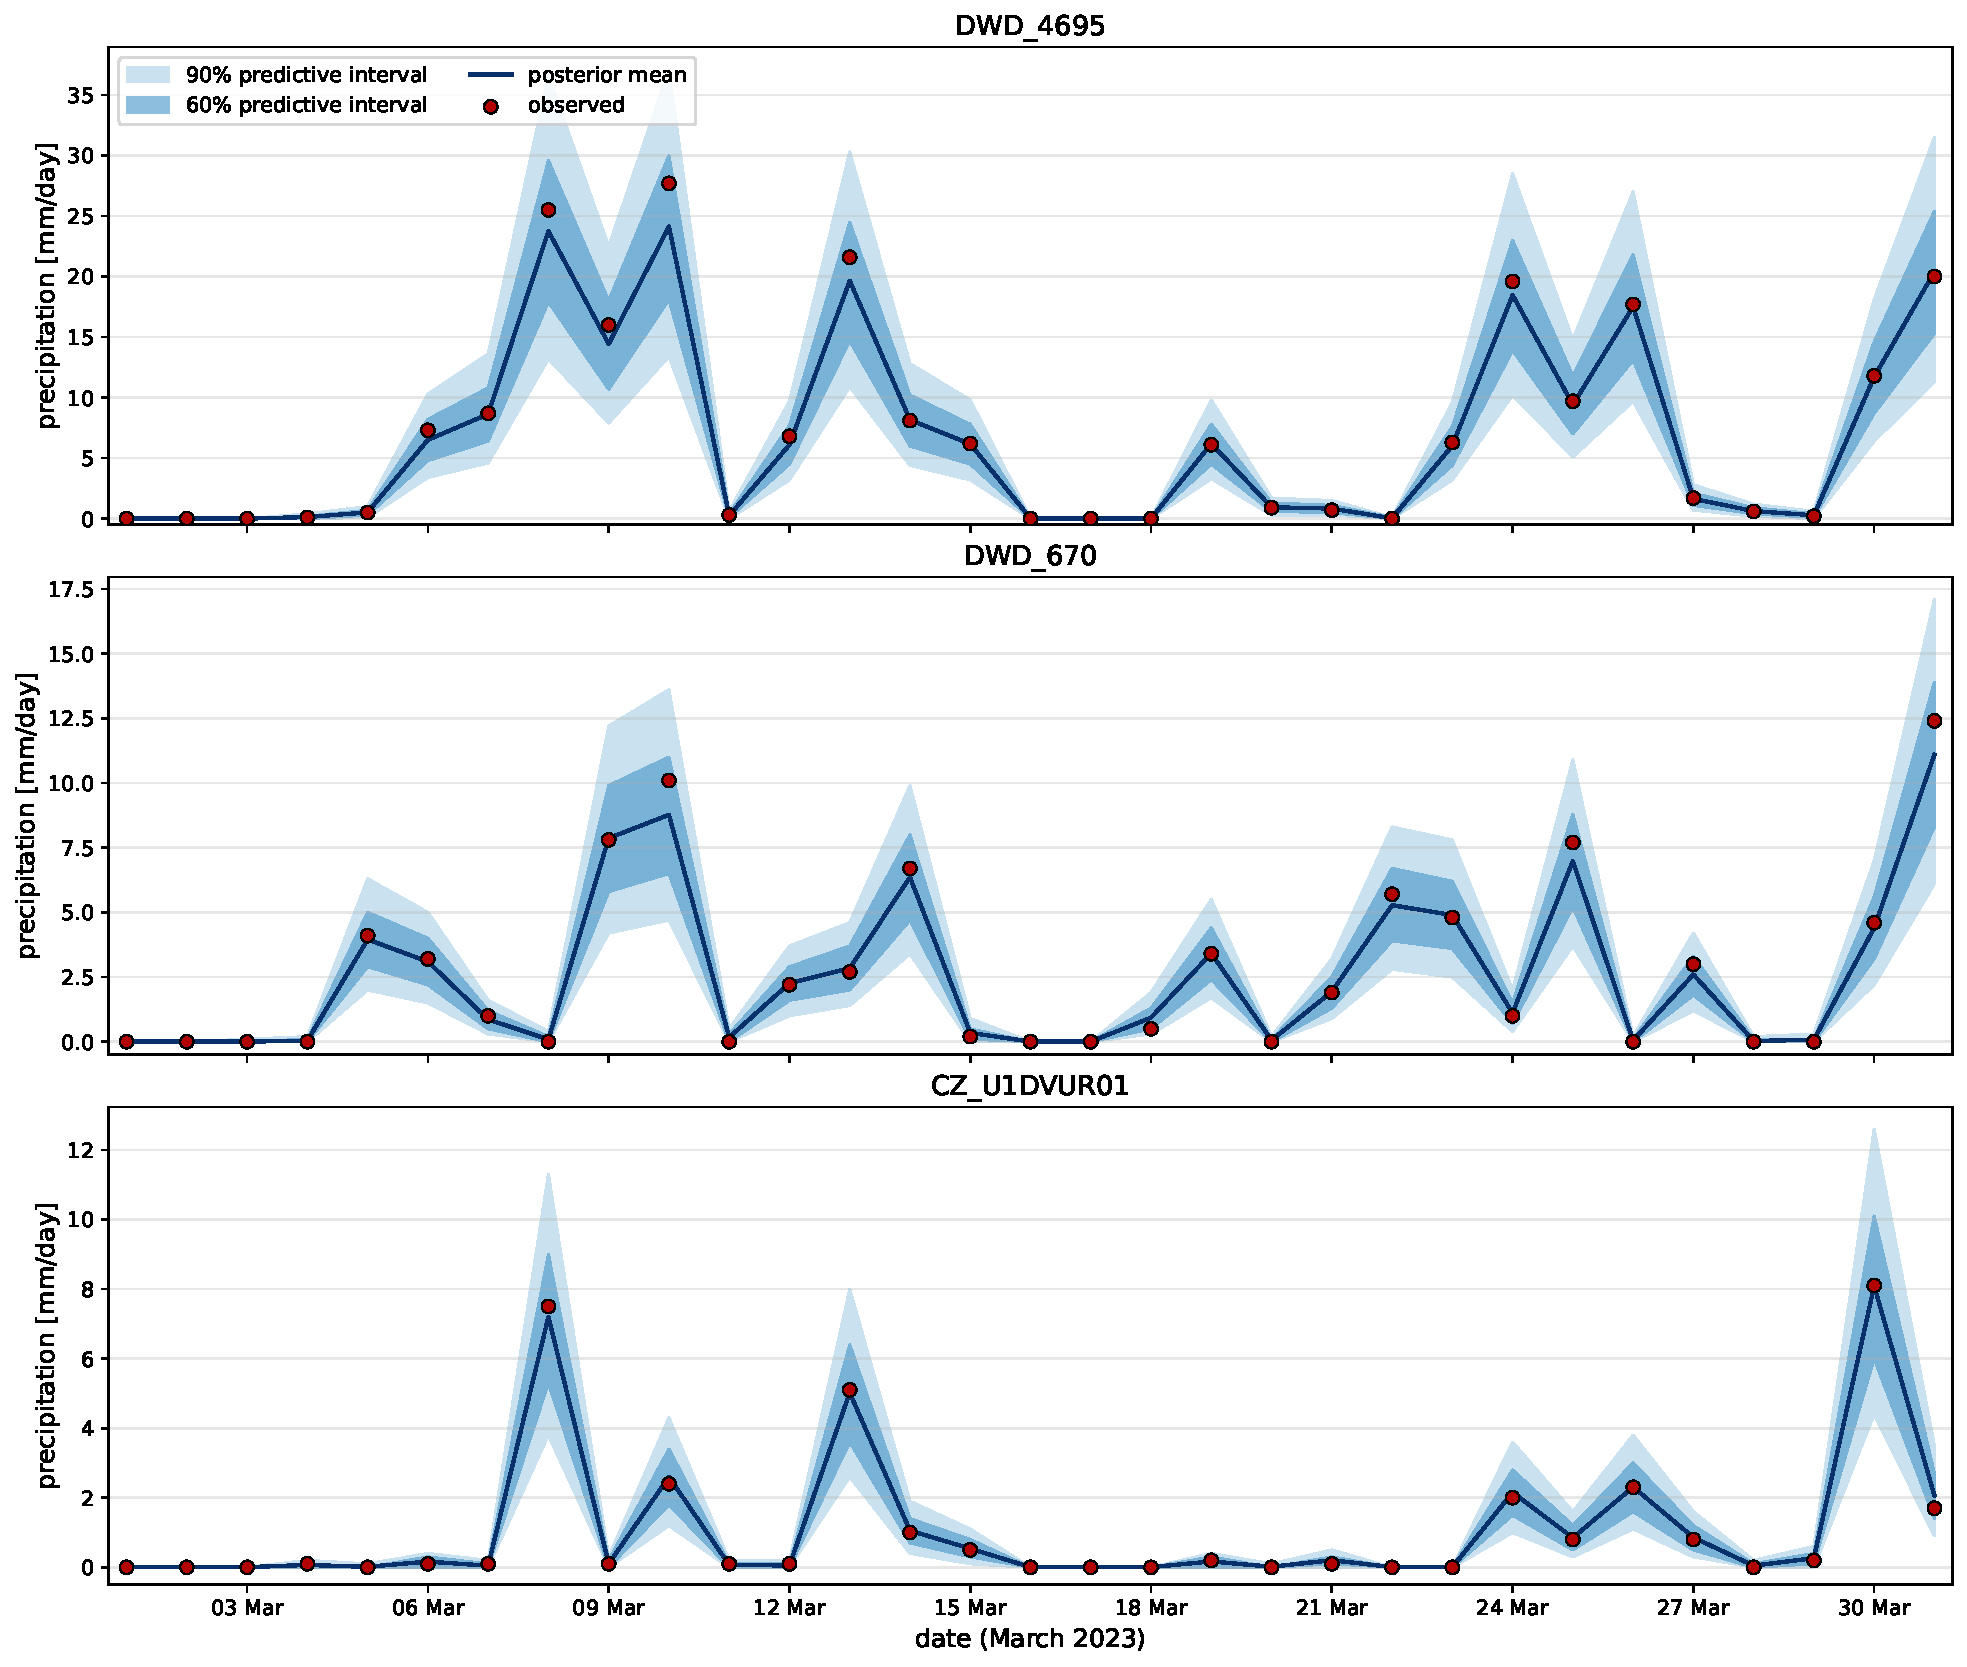
\includegraphics[width=\linewidth]{images/06/bayesnf_station_timeseries.pdf}
  \caption{Posterior mean ($32$ VI replicas), $60$\,\% and $90$\,\%
  predictive intervals, and held-out observations (red dots) over
  March~$2023$ at three holdout stations.}
  \label{fig:bnf-station-timeseries}
\end{figure}

\chapter{Comparison and Discussion}
\label{ch:comparison}

\section{Holdout evaluation protocol}
\label{sec:comparison-protocol}

All three methods of Chapters~\ref{ch:kriging}, \ref{ch:gbm}
and~\ref{ch:bayesnf} (Ordinary Kriging, gradient boosting and Bayesian
Neural Fields) are evaluated on the same fully held-out subset of the
ReKIS network. Before any model fitting, the 2{,}458 quality-controlled
stations are split into 1{,}966 training stations and 492 holdout
stations. The split is identical across the three methods; the holdout
assignment is stored in \texttt{kriging/holdout\_station\_ids.json} on the
project bucket and is consumed by all three evaluation notebooks.

Models are trained on the 1{,}966 training stations only. The holdout
stations are used only at evaluation time, on which CRPS and MAE are
reported in physical millimetres. The predicted-wet rows below restrict
the evaluation to records on which the model predicts rainfall above
$0{.}4$~mm (${\approx}41\,\%$ of the records).

The three methods do not share a common evaluation window. Ordinary
Kriging and gradient boosting are evaluated on the full $1961$--$2023$
record. Bayesian Neural Fields is evaluated on the $2014$--$2023$
ten-year window because training BayesNF at the canonical
hyperparameters of Section~\ref{sec:bayesnf-arch} (32~VI replicas
$\times$ 100 epochs on the long-table input) over the full $63$-year
record exceeded the GPU budget allocated to this thesis. The
$2014$--$2023$ subset is the same window used for the VI-vs-MAP
cross-validation of Section~\ref{sec:bayesnf-vi-vs-map} and corresponds
to the densest decade of the ReKIS network. The cross-method numbers
of Table~\ref{tab:final-comparison} must therefore be read with this
asymmetry in mind: the BayesNF row covers the recent dense decade
rather than the long historical tail of the record.

\section{Cross-model metrics}
\label{sec:comparison-metrics}

Table~\ref{tab:final-comparison} collects the final holdout metrics for
the three methods.

\begin{table}[ht]
  \centering
  \caption{Final holdout metrics on the 492 reserved stations.
  Predicted-wet rows include only records with $\hat{Z} \ge 0{.}4$~mm.
  Ordinary Kriging and gradient boosting are evaluated over the full
  $1961$--$2023$ record; Bayesian Neural Fields over the $2014$--$2023$
  decade only (Section~\ref{sec:comparison-protocol}).}
  \label{tab:final-comparison}
  \begin{tabular}{l l cc}
    \toprule
    Method & Subset & MAE (mm) & CRPS (mm) \\
    \midrule
    Ordinary Kriging   & All records   & 0.480 & 0.384 \\
    Ordinary Kriging   & Predicted-wet & 1.092 & 0.858 \\
    \midrule
    Gradient boosting  & All records   & 0.432 & 0.342 \\
    Gradient boosting  & Predicted-wet & 0.965 & 0.735 \\
    \midrule
    Bayesian Neural Fields & All records   & 0.347 & 0.286 \\
    Bayesian Neural Fields & Predicted-wet & 0.802 & 0.702 \\
    \bottomrule
  \end{tabular}
\end{table}

The ranking is consistent across both error families and across the
all-records and predicted-wet partitions of the holdout set. Bayesian
Neural Fields attains the lowest CRPS and the lowest MAE in every row
of Table~\ref{tab:final-comparison}: relative to Ordinary Kriging it
reduces all-records MAE by $27.7\,\%$ and CRPS by $25.5\,\%$, and
relative to gradient boosting it reduces the same metrics by $19.7\,\%$
and $16.4\,\%$. The improvement persists on the harder predicted-wet
subset, on which BayesNF cuts the kriging CRPS by $18.2\,\%$ and the
gradient-boosting CRPS by $4.5\,\%$. Even after the evaluation-window
caveat of Section~\ref{sec:comparison-protocol} is taken into account
(the BayesNF row is computed on the recent dense decade rather than on
the full historical record), the gap is large enough that the model
remains the strongest of the three on the common $2014$--$2023$ slice,
and it is the only method that produces a calibrated predictive
distribution at every grid cell rather than a point estimate plus a
plug-in variance. On these grounds the Bayesian Neural Field is
selected as the production model for the gridded precipitation product
of the next section.

\section{Multi-resolution gridded product}
\label{sec:comparison-multires}

The selected BayesNF model is applied over the full study domain to
produce a gridded daily precipitation product on the EPSG:3035
projection. Construction proceeds in three steps. First, the same
feature vector that the model expects at training time is recomputed
at every cell of a $1$~km EPSG:3035 lattice over the study area: the
static covariates (projected coordinates, latitude and longitude,
elevation from Copernicus DEM, the six SoilGrids variables) are
sampled once from the rasters, and the dynamic neighbour-derived
features (IDW, GOS and the five SVD-quantile levels
$\mathrm{svd}\_05..\mathrm{svd}\_09$ of
Section~\ref{sec:bayesnf-features}) are recomputed per day, using the
$1{,}966$ training stations as the neighbour pool so that no holdout
station enters the input. Second, the $1$~km feature parquets are
block-mean-aggregated to $2$, $5$ and $10$~km, so that all four nested
target grids share the same domain extent, origin and feature schema.
Third, the trained BayesNF VI ensemble of Chapter~\ref{ch:bayesnf},
fit on the $1{,}966$ training stations only, is run forward on every
(cell, day) feature row and emits a posterior predictive mean in
millimetres together with the standard deviation aggregated over the
$32$ VI replicas. The product is materialised for the month of
March~$2023$ as a worked example covering all four resolutions; the
same pipeline runs unchanged on any other date range.

Figure~\ref{fig:multires-case-day} compares the four resolutions on
the case day $2023$-$03$-$26$. As the cell size grows, two effects
are visible. The first is a progressive smoothing of orographic
gradients along the southern foothills: the sharp wet--dry contrast
that the $1$~km field resolves at the ridgeline is blurred at $5$~km
and largely flattened at $10$~km, because block-mean aggregation of
the input features averages the underlying elevation and neighbour
statistics over progressively larger windows. The second is the
gradual disappearance of small, isolated rain cells in the northern
plain: $1$--$2$~mm pockets that are individually resolved at $1$~km
get diluted into the surrounding dry background as soon as the cell
encompasses several of them, and by $10$~km they are no longer
distinguishable from the climatological field.

\begin{figure}[ht]
  \centering
  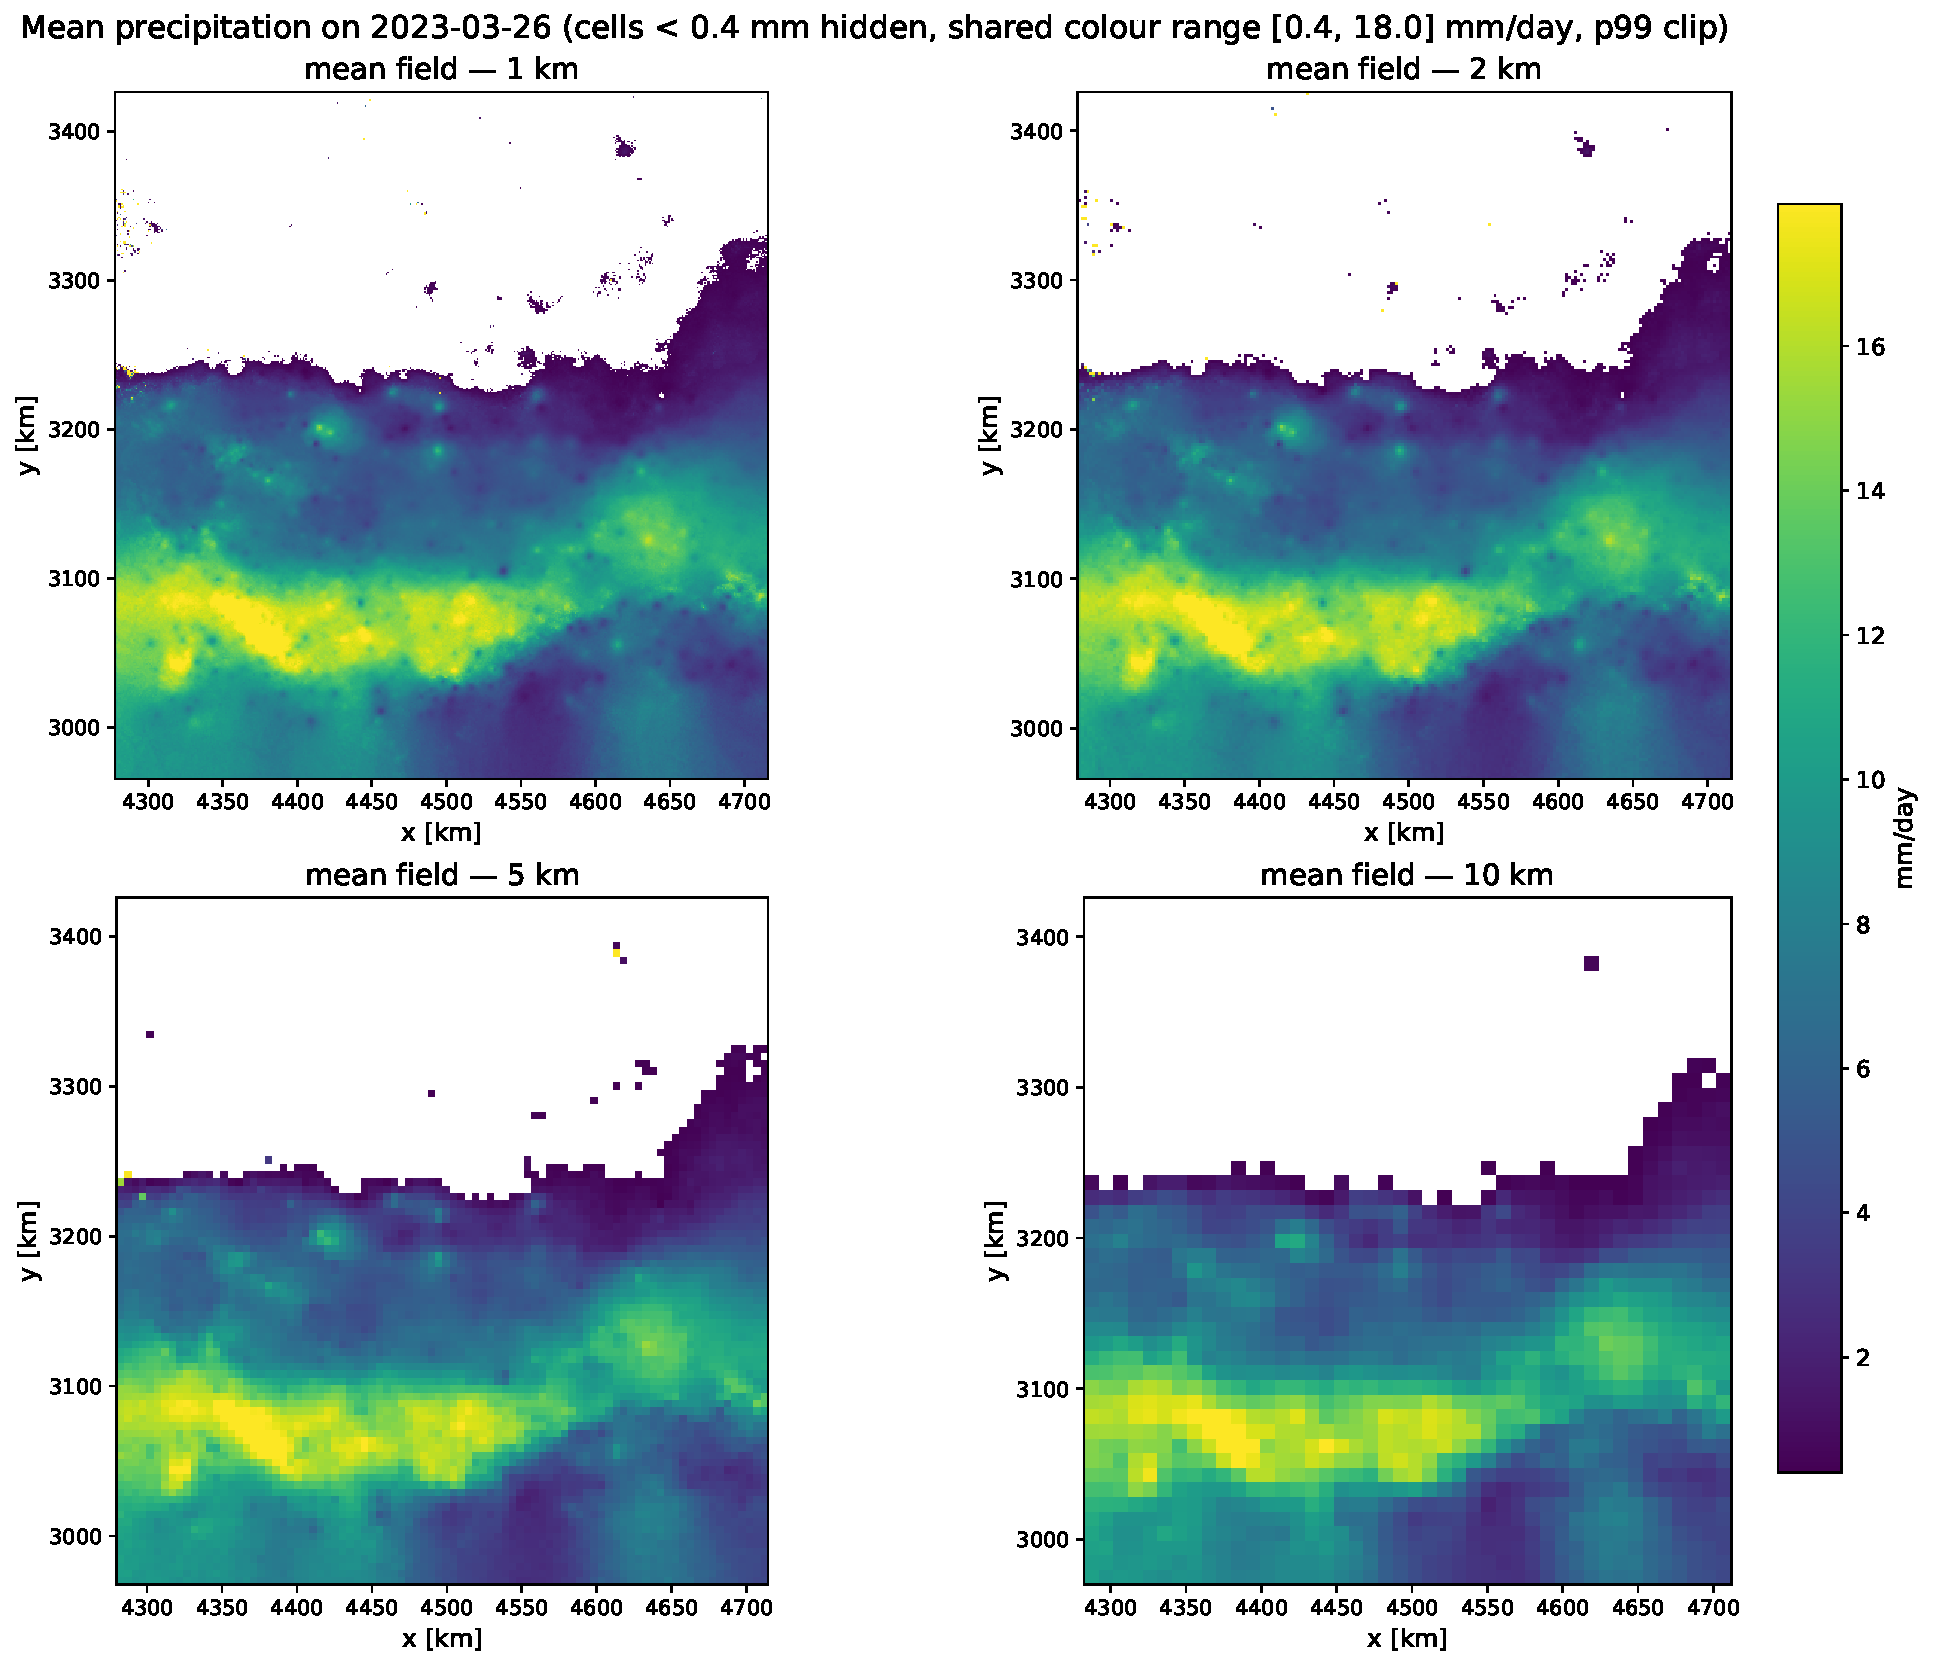
\includegraphics[width=\linewidth]{images/07/multires_case_day.pdf}
  \caption{Posterior mean precipitation on $2023$-$03$-$26$ at the
  four product resolutions ($1$, $2$, $5$ and $10$~km). Cells with
  predicted rainfall below $0.4$~mm are masked. The shared colour
  range $[0.4, 18.0]$~mm clipped at the $99$th percentile lets the
  smoothing of orographic gradients and the gradual loss of small
  isolated rain cells be read off directly between panels.}
  \label{fig:multires-case-day}
\end{figure}

A multi-resolution validation against the holdout stations confirms
that accuracy degrades only modestly with coarsening: holdout MAE
rises from $0.294$~mm at $1$~km to $0.338$~mm at $10$~km, and the bias
between the directly-predicted coarse field and the spatial aggregate
of the $1$~km field stays below $0.02$~mm at every resolution. The
product is distributed as one Parquet file per resolution under
\texttt{results/dataset/predictions\_\{1,2,5,10\}km/}, indexed by
\texttt{(date, cell\_id)}.

\chapter{Conclusion}
\label{ch:conclusion}

This thesis built continuous $1$~km gridded daily precipitation
fields over northern and central Germany from the ReKIS station
network. Three families of estimator were implemented on a common
preprocessing pipeline and evaluated on the same held-out subset of
the network: Ordinary Kriging as the geostatistical baseline,
gradient boosting as a flexible regressor over engineered covariates,
and Bayesian Neural Fields as a probabilistic spatiotemporal model.

The three objectives stated in Chapter~\ref{ch:introduction} were
met as follows. The first objective, implementation and validation
of Ordinary Kriging as a baseline, was fulfilled by the two-stage
indicator-plus-amount pipeline of Chapter~\ref{ch:kriging}, whose
leave-one-out cross-validation under MAE and CRPS established the
geostatistical reference against which the remaining methods are
measured. The second objective, assessment of terrain elevation
as an auxiliary predictor, was addressed in the same chapter
through the elevation-aware monthly normals built on the Copernicus
DEM and confirmed that orographic information reduces the residual
trend prior to spatial interpolation. The third objective,
contextualisation against machine-learning alternatives, was met
by the gradient boosting pipeline of Chapter~\ref{ch:gbm}
and the Bayesian Neural Field of Chapter~\ref{ch:bayesnf}, both
trained and validated on the same data splits as the geostatistical
baseline; the cross-method comparison of Chapter~\ref{ch:comparison}
quantified the trade-off between interpretability and predictive
accuracy and provided the empirical basis for selecting the
Bayesian Neural Field as the production model.

The cross-method evaluation of Chapter~\ref{ch:comparison} confirmed
that the Bayesian Neural Field attains the lowest holdout MAE and CRPS
among the three methods and is the only one of them that returns a
calibrated predictive distribution at every grid cell; gradient
boosting placed between Ordinary Kriging and the Bayesian Neural Field
on both metrics. The selected model was then materialised as a
four-resolution gridded daily precipitation product for the worked
example month and distributed as a Parquet dataset over the four
nested target resolutions.

Inspection of the resulting fields confirmed that the high-resolution
Copernicus DEM and the SoilGrids covariates are a necessary input for
resolving local rainfall: without elevation and soil information at
$1$~km, the orographic and surface-controlled components of local
rainfall collapse into the broad station-distance trend, and the
progressive smoothing observed at coarser resolutions is the direct
expression of this mechanism.

Two limitations of the present work point to natural continuations.
The \texttt{bayesnf} library exposes its model and its variational
inference loop at a fairly low level, so that using the framework to
its full strength requires fluent JAX and a working knowledge of
variational inference and Bayesian model construction; at the present
stage of the author's expertise this is the binding constraint on what
Chapter~\ref{ch:bayesnf} could explore, and the hyperparameter sweep
reported there should be read as a first pass over the configuration
space rather than as a settled tuning. A more principled second round
of model tuning, a deeper analysis of the covariate stack already
introduced in Chapter~\ref{ch:bayesnf}, and a direct cross-check of
the gridded product against established national gridded precipitation
datasets would situate the present results among existing operational
references and identify in which regimes and regions the proposed
pipeline improves on or falls behind them.
 % include `text.tex'

\appendix\appendixinit % do not remove these two commands

\chapter{Contents of the attached archive}
\label{app:archive}

The reproduction archive shipped with the thesis contains the trained
models, the summary cross-validation metrics, and the gridded precipitation
product for the worked-example year~2023. Raw inputs (ReKIS station files,
the Copernicus DEM, SoilGrids rasters) and per-fold intermediate files are
excluded; they can be regenerated from the public sources by running the
pipeline scripts of the repository (Appendix~\ref{app:repo}).

\medskip\noindent\textbf{Note on availability.} The compressed archive
exceeds the $4$~GB upload limit of the faculty submission system and is
therefore not attached to this thesis directly. It is available on request;
the author can be contacted at \texttt{ismaktam@fit.cvut.cz}. The same
artefacts can also be regenerated by running the pipeline scripts of the
public repository against the project S3 bucket (Appendix~\ref{app:repo}).
The directory tree below documents the layout the archive follows.

\dirtree{%
.1 source/.
.2 README.md\DTcomment{layout, load snippets, list of omissions}.
.2 kriging/\DTcomment{Ordinary Kriging baseline (Chapter~\ref{ch:kriging})}.
.3 global\_variogram.pkl\DTcomment{fitted spherical and exponential variograms}.
.3 winner.json\DTcomment{selected transform $\times$ variogram combination}.
.3 holdout\_station\_ids.json\DTcomment{492 holdout station identifiers shared by all three methods}.
.3 kfold/cv\_results.json\DTcomment{5-fold MAE/CRPS summary}.
.3 test/.
.4 holdout\_predictions.parquet\DTcomment{492-station holdout predictions, 1961--2023}.
.4 test\_metrics.json\DTcomment{Table~\ref{tab:final-comparison} row}.
.2 lgbm/\DTcomment{Gradient boosting (Chapter~\ref{ch:gbm})}.
.3 final/.
.4 stage1.joblib\DTcomment{wet/dry binary classifier}.
.4 models.joblib\DTcomment{11 quantile regressors of the amount stage}.
.4 features.parquet\DTcomment{training feature matrix}.
.3 hparam/\DTcomment{HPO best parameters, grid results, sweep plots}.
.3 kfold/cv\_results.json\DTcomment{5-fold MAE/CRPS summary}.
.3 fold\_assignment.parquet\DTcomment{shared 5-fold split, used by all three methods}.
.3 oof\_predictions.parquet\DTcomment{out-of-fold predictions on training stations}.
.3 uncertainty\_fold0.json\DTcomment{quantile-spread diagnostics}.
.2 bayesnf/\DTcomment{Bayesian Neural Field (Chapter~\ref{ch:bayesnf})}.
.3 runs/vi\_\_final\_\_WY\_h1\_10\_\_ffrk\_full/.
.4 model.pkl\DTcomment{32-replica variational ensemble}.
.4 metrics.json.
.4 losses.npy\DTcomment{ELBO trace}.
.4 preds.parquet\DTcomment{holdout predictions}.
.3 final/features.parquet\DTcomment{training feature matrix}.
.3 kfold\_summary\_vi.json\DTcomment{5-fold VI summary}.
.3 kfold\_summary\_map.json\DTcomment{5-fold MAP comparison}.
.2 dataset/\DTcomment{multi-resolution gridded product, worked-example month (March 2023)}.
.3 grid\_\{2,5,10\}km\_static.parquet\DTcomment{cell geometry, elevation, soil; at 1\,km the static features are embedded in each monthly file}.
.3 grid\_\{1,2,5,10\}km/2023-03.parquet\DTcomment{input covariate stack for the worked example}.
.3 predictions\_\{1,2,5,10\}km/2023-03.parquet\DTcomment{predicted gridded fields}.
}

Loading each artefact is documented in \texttt{source/README.md}; in short,
the kriging variogram and the Bayesian Neural Field ensemble are unpickled,
the gradient-boosting boosters are read with \texttt{joblib.load}, and the
gridded product is read directly with \texttt{pandas.read\_parquet}. The
Python environment required to load the boosters and the Bayesian Neural
Field is installed from the repository root with
\texttt{pip install -e ".[cpu]"}.

\chapter{Source-code repository}
\label{app:repo}

The full source code, the experimental notebooks, the AWS execution
scripts, and the \LaTeX{} sources of the present document are released as a
public Git repository~\cite{thesisRepo}. The top-level layout is:

\dirtree{%
.1 precip\_interpolation\_thesis/.
.2 src/thesis/\DTcomment{installable Python package}.
.3 config.py\DTcomment{single source of truth for hyperparameters}.
.3 data/\DTcomment{ReKIS, DEM, SoilGrids loaders}.
.3 datasets/\DTcomment{per-day station dataset, prediction grid}.
.3 transforms/\DTcomment{Projection $\to$ Indicator $\to$ Detrend $\to$ NormalScore}.
.3 models/kriging/\DTcomment{two-stage Ordinary Kriging, variogram fitter, LOO-CV}.
.3 evaluation/\DTcomment{MAE/CRPS metrics, scoring helpers}.
.3 scripts/\DTcomment{pipeline entry points; one CLI per experiment}.
.2 notebooks/\DTcomment{experimental and pedagogical notebooks}.
.3 01\_data/\DTcomment{exploratory data analysis, dataset construction}.
.3 02\_methodology/\DTcomment{methodological derivations and demonstrations}.
.3 03\_kriging/\DTcomment{variogram fitting, LOO-CV, sensitivity}.
.3 04\_lgbm/\DTcomment{HPO sweep, 5-fold CV, final model, multi-resolution demo}.
.3 05\_bayesnf/\DTcomment{baseline, geo and time ablations, k-fold, final run}.
.3 06\_comparison/\DTcomment{cross-method evaluation against the held-out set}.
.3 07\_dataset/\DTcomment{multi-resolution gridded product generation}.
.2 scripts/\DTcomment{cloud orchestration (Docker, AWS, Vast.ai)}.
.3 entrypoint.sh\DTcomment{Docker entry point used on the GPU workers}.
.3 fetch\_source.sh\DTcomment{mirrors the curated S3 subset into source/}.
.2 thesis/\DTcomment{\LaTeX{} sources of the present document}.
.2 pyproject.toml\DTcomment{package metadata, CPU and GPU extras}.
.2 Dockerfile\DTcomment{CUDA 12.1, Python 3.12, uv}.
}

The pipeline is fully reproducible from this repository. After exporting
the AWS credentials documented in the repository \texttt{README}, the
script sequence
\texttt{run\_variogram}~$\to$~\texttt{build\_monthly\_grids}~$\to$~\texttt{run\_cv}
regenerates the kriging baseline. The notebook directories \texttt{04\_lgbm/}
and \texttt{05\_bayesnf/} regenerate the two machine-learning models, and
\texttt{07\_dataset/} regenerates the gridded product distributed in the
attached archive.
 % include `appendix.tex'

\backmatter % do not remove this command

\begin{sloppypar}
\printbibliography % print out the BibLaTeX-generated bibliography list
\end{sloppypar}

\include{medium} % include `medium.tex'

\end{document}
